% =============================================================================
% EpiForecast-MX — Avance 5: Modelo Final (Ensemble Learning)
% Equipo 01 — Maestria en Inteligencia Artificial Aplicada (MNA)
% Tecnologico de Monterrey x Instituto Mexicano del Seguro Social
% =============================================================================
\documentclass[12pt, letterpaper]{article}

% -- Paquetes ----------------------------------------------------------------
\usepackage[utf8]{inputenc}
\usepackage[T1]{fontenc}
\usepackage[spanish,es-tabla]{babel}
\usepackage{geometry}
\geometry{letterpaper, margin=2.5cm, top=3cm, bottom=2.5cm}
\usepackage{graphicx}
\usepackage{float}
\usepackage{booktabs}
\usepackage{tabularx}
\usepackage{longtable}
\usepackage{multirow}
\usepackage{xcolor}
\usepackage{colortbl}
\usepackage{fancyhdr}
\usepackage{titlesec}
\usepackage{enumitem}
\usepackage{amsmath, amssymb}
\usepackage{caption}
\usepackage{subcaption}
\usepackage[most]{tcolorbox}
\usepackage{fontawesome5}
\usepackage{pifont}
\usepackage{parskip}
\usepackage{setspace}
\usepackage{array}
\usepackage[bottom]{footmisc}
\usepackage{xurl}          % URLs con salto de linea automatico
\usepackage[breaklinks=true]{hyperref}

% -- Colores institucionales IMSS / EpiForecast ------------------------------
\definecolor{burgundy}{HTML}{9B2242}
\definecolor{darkburgundy}{HTML}{6F1D46}
\definecolor{teal}{HTML}{00524E}
\definecolor{darkteal}{HTML}{173F35}
\definecolor{gold}{HTML}{B58500}
\definecolor{coolgray}{HTML}{97999B}
\definecolor{imssblue}{HTML}{003A70}
\definecolor{cream}{HTML}{F5EDE0}
\definecolor{lightgreen}{HTML}{E6F4EA}
\definecolor{lightyellow}{HTML}{FEF7E0}
\definecolor{lightred}{HTML}{FDE8E8}

% Colores especificos por Motor MLOps
\definecolor{cprophet}{HTML}{004D40}
\definecolor{cdeepar}{HTML}{880E4F}
\definecolor{censemble}{HTML}{FF6F00}
\definecolor{cstacking}{HTML}{1A237E}

% -- Configuracion de hyperref -----------------------------------------------
\hypersetup{
    colorlinks=true,
    linkcolor=teal,
    citecolor=burgundy,
    urlcolor=imssblue,
    bookmarksopen=true,
    pdftitle={EpiForecast-MX -- Avance 5: Modelo Final},
    pdfauthor={Equipo 01 -- MNA Tec de Monterrey},
}

% -- Headers y footers -------------------------------------------------------
\pagestyle{fancy}
\fancyhf{}
\fancyhead[L]{\small\textcolor{coolgray}{EpiForecast-MX -- Avance 5: Modelo Final}}
\fancyhead[R]{\small\textcolor{coolgray}{Equipo 01 -- MNA -- Tec de Monterrey}}
\fancyfoot[C]{\thepage}
\fancyfoot[R]{\small\textcolor{coolgray}{Marzo 2026}}
\renewcommand{\headrulewidth}{0.4pt}
\renewcommand{\footrulewidth}{0.2pt}

% -- Titulos con colores IMSS ------------------------------------------------
\titleformat{\section}
  {\Large\bfseries\color{teal}}{\thesection.}{0.5em}{}[\vspace{-0.5em}\textcolor{teal}{\rule{\textwidth}{1pt}}]
\titleformat{\subsection}
  {\large\bfseries\color{burgundy}}{\thesubsection}{0.5em}{}
\titleformat{\subsubsection}
  {\normalsize\bfseries\color{darkteal}}{\thesubsubsection}{0.5em}{}

% -- Cajas de callout --------------------------------------------------------
\newtcolorbox{insightbox}[1][]{
  colback=lightgreen, colframe=teal,
  boxrule=0pt, leftrule=4pt, arc=2pt,
  fonttitle=\bfseries, title=#1
}
\newtcolorbox{warningbox}[1][]{
  colback=lightyellow, colframe=gold,
  boxrule=0pt, leftrule=4pt, arc=2pt,
  fonttitle=\bfseries, title=#1
}
\newtcolorbox{criticalbox}[1][]{
  colback=lightred, colframe=burgundy,
  boxrule=0pt, leftrule=4pt, arc=2pt,
  fonttitle=\bfseries, title=#1
}

% Caja de Campeon en Produccion (Dorada)
\newtcolorbox{championbox}[1][]{
  colback=white, colframe=gold,
  boxrule=2pt, arc=6pt,
  fonttitle=\bfseries\large, coltitle=black,
  title={\textcolor{gold}{\faTrophy}\ \textbf{Modelo Campeon en Produccion} #1}
}

% -- Comandos personalizados -------------------------------------------------
\newcommand{\smape}{\textsc{smape}}
\newcommand{\mase}{\textsc{mase}}
\newcommand{\rmse}{\textsc{rmse}}
\newcommand{\imss}{\textsc{imss}}
\newcommand{\tabref}[1]{Tabla~\ref{#1}}
\newcommand{\figref}[1]{Figura~\ref{#1}}
\newcommand{\secref}[1]{Seccion~\ref{#1}}

\begin{document}

% =============================================================================
% PORTADA
% =============================================================================
\begin{titlepage}
\begin{center}

\vspace*{0.5cm}

% Logos institucionales (subir a Overleaf: logo_tec.png y logo_imss.png)

\includegraphics[height=2cm]{logo_tec.png}\hspace{2cm}
\includegraphics[height=2.5cm]{logo_imss.png}

\vspace{0.5cm}

{\small Instituto Tecnologico y de Estudios Superiores de Monterrey}\\[0.1cm]
{\small Maestria en Inteligencia Artificial Aplicada (MNA)}\\[0.5cm]

\textcolor{teal}{\rule{\textwidth}{2pt}}\\[0.4cm]
{\Huge\bfseries\textcolor{teal}{EpiForecast-MX}}\\[0.2cm]
{\LARGE\textcolor{burgundy}{Avance 5: Modelo Final (Ensemble Learning)}}\\[0.3cm]
\textcolor{teal}{\rule{\textwidth}{2pt}}\\[0.8cm]

{\large\textit{Generalizacion de modelos nacionales de pronostico epidemiologico\\hacia un enfoque modular con desagregacion por sexo y\\entidad federativa en Mexico}}\\[1.2cm]

{\large\textbf{Materia:} Proyecto Integrador -- TC5035.10}\\[0.5cm]

\begin{tabular}{ll}
\textbf{Asesora:}     & Dra.\ Grettel Barcelo Alonso \\
\textbf{Director MNA:}& Dr.\ Luis Eduardo Falcon Morales \\
\textbf{Profesora:}   & Mtra.\ Veronica Sandra Guzman de Valle \\
\textbf{IMSS:}        & Dra.\ Ruth Perez-Hernandez (Lider de Proyecto) \\
                      & Dra.\ Lina Diaz Castro (Investigadora en Psiquiatria) \\
\end{tabular}\\[1cm]

\textbf{\Large Equipo 01}\\[0.4cm]
\begin{tabular}{lll}
\textbf{Javier A. Rebull Saucedo} & A01795838 & Sr.\ Assoc.\ Dev.\ -- Santander Bank US \\
\textbf{Juan Carlos Perez Nava}   & A01795941 & Head of Area -- IMSS \\
\textbf{Luis G. Sanchez Salazar}  & A01232963 & Sr.\ Controls Engineer -- Tesla \\
\end{tabular}\\[1.0cm]

{\large Marzo 2026}

\end{center}
\end{titlepage}

% =============================================================================
% TABLA DE CONTENIDOS
% =============================================================================
\newpage
\tableofcontents
\newpage

% =============================================================================
% 1. INTRODUCCION Y RESPUESTA A RETROALIMENTACION
% =============================================================================
\section{Introduccion y Acciones Correctivas}\label{sec:intro}

El presente documento detalla la consolidacion algoritmica del ecosistema \textbf{EpiForecast-MX} (Avance~5). En cumplimiento de los Objetivos 3.5 y 3.6, el sistema evoluciona desde modelos \textit{baseline} individuales hacia un framework completo de \textbf{Ensemble Learning} con estrategias homogeneas y heterogeneas, evaluando un total de \textbf{1,332 modelos} (4 motores $\times$ 333 combinaciones clinicas) sobre \textbf{630 semanas} de datos historicos (2013--2026) para potenciar la precision clinica en el Instituto Mexicano del Seguro Social (\imss{}).

El sistema pronostica la incidencia semanal de tres padecimientos neurologicos y psiquiatricos ---\textbf{Depresion (F32)}, \textbf{Parkinson (G20)} y \textbf{Alzheimer (G30)}--- para las \textbf{32 entidades federativas}, desagregados por sexo, con un horizonte de \textbf{52 semanas}.

A partir de la retroalimentacion provista por la Dra.\ Grettel Barcelo en el avance anterior, el equipo implemento mejoras estructurales criticas:

\begin{table}[H]
\centering
\caption{Atencion a la retroalimentacion y acciones correctivas implementadas}
\label{tab:feedback}
\small
\begin{tabularx}{\textwidth}{>{\bfseries\hsize=.35\hsize}X >{\hsize=.65\hsize}X}
\toprule
Comentario / Hallazgo & Resolucion MLOps Implementada \\
\midrule
\rowcolor{lightgreen!20}
Aclarar el origen de los 312 (ahora 333) modelos base. & \textcolor{teal}{\ding{51}} \textbf{Matematica de la red:} 3 padecimientos $\times$ (32 estados + 4 regiones fallback + 1 nacional) $\times$ 3 sexos = \textbf{111 series por motor}. Al competir 4 motores, el sistema evalua 444 combinaciones, pero en produccion se inyectan estrictamente \textbf{333 modelos ganadores} (uno por serie). \\
\addlinespace
Reemplazar MAPE por SMAPE debido a la inflacion por ceros. & \textcolor{teal}{\ding{51}} \textbf{SMAPE como metrica primaria:} SMAPE $= \frac{2|y - \hat{y}|}{|y| + |\hat{y}|}$ penaliza de forma simetrica y no se infla al infinito con los ceros de Alzheimer y Parkinson. Es la metrica de seleccion automatica en produccion. \\
\addlinespace
\rowcolor{lightgreen!20}
Prophet se ve plano fuera de pandemia. Faltan picos. & \textcolor{teal}{\ding{51}} \textbf{Diversificacion algoritmica:} Prophet es propenso al suavizado lineal. Con \textbf{DeepAR} (LSTM) y \textbf{Ensemble con XGBoost}, el sistema captura la varianza de corto plazo y los picos estacionales reales. \\
\addlinespace
El Dashboard muestra Casos Absolutos en vez de Tasas. & \textcolor{teal}{\ding{51}} \textbf{Diseno clinico deliberado:} El sistema entrena internamente con tasas (por 100k hab.) para aislar la demografia. Al predecir, \textbf{desnormaliza} multiplicando por poblacion. Tableau muestra \textbf{casos absolutos} porque el IMSS planea camas e insumos con pacientes, no con tasas. \\
\addlinespace
\rowcolor{lightgreen!20}
Separar niveles territoriales en los filtros de la UI. & \textcolor{teal}{\ding{51}} \textbf{Refactorizacion UI:} Tableau ahora muestra las 32 entidades en un combo independiente. Las regiones INEGI y la vista nacional tienen vistas separadas. \\
\addlinespace
Frecuencia de re-entrenamiento. & \textcolor{teal}{\ding{51}} \textbf{Politica de Produccion:} Pronosticos a \textbf{52 semanas}, con re-entrenamiento parametrico programado de forma \textbf{trimestral}. \\
\bottomrule
\end{tabularx}
\end{table}

\newpage

% =============================================================================
% 2. MARCO TEORICO Y DISENO DE ENSAMBLES
% =============================================================================
\section{Marco Teorico y Diseno de Ensambles}\label{sec:marco}

\subsection{Filosofia del Ensemble Learning}
El aprendizaje por ensamble (\textit{Ensemble Learning}) combina multiples aprendices base para producir un pronostico superior y mas generalizable~[1]. En series de tiempo epidemiologicas, donde la varianza interestatal es alta y el impacto del COVID-19 genero rupturas de regimen, un modelo individual suele caer en el dilema de sesgo-varianza~[2].

Para EpiForecast-MX, disenamos una bateria de motores que ataca ambos frentes: tecnicas de \textbf{redes multi-serie} para estabilizar la varianza y \textbf{Boosting/Stacking} para reducir el sesgo.

\subsection{Arquitectura de los 4 Motores de Pronostico}

El sistema pone a competir 4 arquitecturas radicalmente distintas (\tabref{tab:motores}):

\begin{table}[H]
\centering
\caption{Arquitectura de los 4 Motores de Pronostico (Objetivo 3.5)}
\label{tab:motores}
\small
\begin{tabularx}{\textwidth}{>{\raggedright\arraybackslash}p{1.8cm} >{\raggedright\arraybackslash}p{2.2cm} X}
\toprule
\textbf{Motor} & \textbf{Estrategia} & \textbf{Descripcion Tecnica} \\
\midrule
\rowcolor{cprophet!10}
\textbf{Prophet} & Baseline individual & Modelo aditivo bayesiano (Meta/Facebook). Descomposicion: tendencia (logistica segmentada con 12--25 \textit{changepoints}) + estacionalidad anual (series de Fourier, orden 10) + regresores (holiday COVID: 913 dias). Validacion cruzada con 4 folds temporales y pesos progresivos $[0.5, 0.75, 1.0, 1.25]$. Aplica $\log(1+y)$ y normaliza a tasa por 100k habitantes. \\
\addlinespace
\rowcolor{cdeepar!10}
\textbf{DeepAR} & Ensamble homogeneo (multi-serie) & Red neuronal LSTM autoregresiva probabilistica~[3]. Implementada sobre GluonTS + PyTorch. Entrena las 32 series estatales \textbf{simultaneamente}, aprendiendo correlaciones espaciales via \textit{transfer learning}. Arquitectura: 2 capas LSTM, 80 celdas, dropout 0.15, distribucion Student-$t$. Contexto de 104 semanas (2 anos), 200 muestras Monte Carlo para intervalos de confianza. \\
\addlinespace
\rowcolor{censemble!10}
\textbf{Ensemble} & Heterogeneo paralelo & Combina la tendencia estacional de \textbf{Prophet} con la correccion de \textbf{XGBoost} alimentado con 20 \textit{features} temporales (7 lags, 5 medias moviles, tasa de cambio, ciclicos seno/coseno, flag COVID). Los pesos se aprenden via regresion \textbf{Ridge} sobre predicciones Out-of-Fold (4 folds, ventana expansiva). Grid search de 36 combinaciones. \\
\addlinespace
\rowcolor{cstacking!10}
\textbf{Stacking} & Heterogeneo generalizado & Une a 3 expertos independientes: \textbf{Prophet}, \textbf{ETS} (Holt-Winters, periodo 52) y \textbf{LightGBM} (300 arboles, profundidad 4). El meta-learner \textbf{ElasticNet} ($\alpha=1.0$, $L_1$-ratio$=0.5$, pesos $\geq 0$) inyecta variables $\sin(2\pi w/52)$ y $\cos(2\pi w/52)$ para decidir en que epoca del ano confiar mas en cada experto. \\
\bottomrule
\end{tabularx}
\end{table}

\begin{insightbox}[Hallazgo Empirico: El Paradigma Macro vs.\ Micro]
Se comprobo empiricamente una ley matematica en el sistema:
\begin{itemize}[noitemsep]
    \item A nivel \textbf{Micro} (estatal, alta varianza, series de 0--5 casos/semana), \textbf{DeepAR} gana abrumadoramente al ``tomar prestada'' informacion espacial de otros estados. Gana en el \textbf{97.3\%} de las series de Depresion y \textbf{83.8\%} de Parkinson.
    \item A nivel \textbf{Macro} (Nacional, senal suavizada por la Ley de los Grandes Numeros), los meta-modelos heterogeneos (\textbf{Ensemble y Stacking}) exprimen mayor precision al combinar logicas lineales con arboles de decision.
\end{itemize}
\end{insightbox}

\newpage

% =============================================================================
% 3. DESAFIOS TECNICOS Y LECCIONES APRENDIDAS
% =============================================================================
\section{Desafios Tecnicos y Lecciones Aprendidas}\label{sec:desafios}

El camino hacia los 1,332 modelos no fue lineal. A continuacion se documentan los obstaculos tecnicos mas significativos y las soluciones de ingenieria que el equipo diseno para superarlos.

\subsection{El Fantasma del Data Leakage en DeepAR}\label{subsec:leakage}

\begin{criticalbox}[Alerta Critica: Deteccion y Eliminacion de Fuga de Datos]
Durante la auditoria de calidad, el equipo descubrio que \textit{GluonTS} (el backend de DeepAR) \textbf{no genera fitted values historicos de forma nativa}. Ante su ausencia, el pipeline original copiaba los valores reales ($y$) como prediccion ($\hat{y}$), produciendo un \smape{} \textit{in-sample} del \textbf{0\%}: una falsa perfeccion que habria invalidado cualquier diagnostico de overfitting entregado al \imss{}.
\end{criticalbox}

\textbf{Solucion --- Backtest por Ventana Expansiva (\textit{Expanding-Window}):} Se programo un procedimiento estricto de retrovalidacion. A partir de la semana 53, el motor retrocede en el tiempo, bloquea su conocimiento del futuro y realiza inferencias en bloques del tamano del horizonte (52 semanas). Para la variante multi-serie (32 estados simultaneos), donde un \textit{backtest} completo por ventana expansiva habria requerido $32 \times N$ pasadas de GPU, se implemento una estrategia hibrida: valores reales para la mayor parte del historial y un unico paso de \textit{backtest} honesto sobre las ultimas 52 semanas de entrenamiento.

El costo computacional se incremento significativamente (de $\sim$1 hora a $\sim$4 horas en macOS M2, o $\sim$1.5 horas en AWS SageMaker con GPU NVIDIA T4), pero aseguro que el diagnostico entregado al \imss{} sea \textbf{estadisticamente honesto} y que las bandas de confianza reflejen incertidumbre real, no ruido de entrenamiento.

\subsection{El Cold Start de DeepAR en Series de Bajo Volumen}\label{subsec:coldstart}

\begin{warningbox}[Cold Start: Cuando la Red Neuronal No Tiene Suficiente Senal]
Las series de \textbf{Alzheimer (G30)} representan el peor escenario para una red neuronal: estados como Baja California Sur, Tlaxcala o Campeche registran \textbf{0--2 casos por semana}. Con 630 semanas de historial donde el 60\% son ceros, la LSTM enfrenta un problema clasico de \textit{cold start}: la senal estadistica es insuficiente para que los gradientes converjan de forma significativa.
\end{warningbox}

\textbf{Solucion --- Modelado Hibrido con Fallback Regional:}
\begin{enumerate}[noitemsep]
    \item Las series con incidencia $<5$ casos en 52 semanas se detectan automaticamente.
    \item Se reasignan al modelo de su \textbf{region INEGI} (Metropolitana, Urbana, Sur-Sureste o Rural), que agrega la senal de multiples estados.
    \item En produccion, \textbf{8 de las 333 series} requirieron este fallback (todas de Alzheimer y una de Parkinson/Campeche).
\end{enumerate}

Esto asegura cobertura del 100\% sin forzar modelos estadisticamente fragiles sobre datos insuficientes.

\subsection{La Convergencia Fallida del ElasticNet (Stacking)}\label{subsec:convergence}

\begin{criticalbox}[Bug Critico: ElasticNet Muere en Series de Ceros]
Al entrenar el Stacking sobre series de Alzheimer (bajo volumen, mayoría ceros), el meta-learner \textbf{ElasticNet} lanzaba \texttt{ConvergenceWarning} y el proceso moria con \textit{leaked semaphores} de \texttt{joblib/loky}. El problema: los folds Out-of-Fold producian vectores de validacion casi constantes (todo ceros), donde el optimizador no encontraba gradiente.
\end{criticalbox}

\textbf{Solucion de 7 capas de defensa:}
\begin{enumerate}[noitemsep]
    \item \textbf{Guardia de varianza minima:} Si $\sigma(y_{\text{oof}}) < 10^{-8}$, asignar pesos uniformes ($1/n$) sin intentar optimizar.
    \item \textbf{Aumento de iteraciones:} De 1,000 (default) a \textbf{10,000} con tolerancia explicita ($10^{-4}$).
    \item \textbf{Filtro por fold:} Saltar folds individuales donde la validacion es constante.
    \item \textbf{Captura de warnings:} Registrar en \texttt{loguru} sin abortar el pipeline.
    \item \textbf{Fallback robusto:} Si Ridge tambien falla, devolver pesos uniformes.
    \item \textbf{Supresion de semaforos filtrados:} Limpieza de recursos del pool de procesos.
    \item \textbf{Propagacion desde config:} Los parametros \texttt{max\_iter} y \texttt{tol} se controlan desde \texttt{stacking.yaml}.
\end{enumerate}

Tras estas 7 mitigaciones, el Stacking completa las 333 series sin excepciones.

\subsection{Fuga de Datos en el Feature Engineering del Ensemble}\label{subsec:fuga_features}

Una segunda fuente de leakage mas sutil se descubrio en el preprocesamiento de datos: la funcion \texttt{\_ajusta\_negativos()} usaba \texttt{shift(-1)} para mirar \textbf{una semana hacia el futuro} al interpolar valores negativos. En la frontera train/test, esto contaminaba el set de entrenamiento con informacion del test, inflando las metricas entre un 5\% y un 15\%.

\textbf{Solucion:} Se reemplazo la interpolacion bidireccional por una \textbf{media movil retrospectiva de 3 semanas} que solo usa datos pasados. Ademas, los features de tasa de cambio (\texttt{roc\_4} y \texttt{roc\_52}) del XGBoost se recalcularon sobre valores \textit{shifted} ($y_{t-1}$) para garantizar que ningun feature accede a $y_t$ en el momento de la prediccion.

Se anadio un test unitario dedicado (\texttt{test\_roc\_no\_leakage}) que verifica matematicamente la ausencia de fuga en cada columna del feature builder.

\newpage

% =============================================================================
% 4. OPTIMIZACION DE HIPERPARAMETROS
% =============================================================================
\section{Optimizacion de Hiperparametros}\label{sec:opt}

\subsection{Prophet: Validacion Cruzada Temporal Ponderada}

Se evaluaron entre 6 y 24 combinaciones de hiperparametros por padecimiento mediante \textbf{TimeSeriesSplit} con 4 folds temporales (test de 53 semanas cada uno). Los folds recientes reciben mayor peso $[0.5, 0.75, 1.0, 1.25]$ para priorizar el comportamiento post-pandemia.

\begin{table}[H]
\centering
\caption{Distribucion de hiperparametros optimos de Prophet (333 modelos)}
\label{tab:prophet_hp}
\small
\begin{tabular}{lcc}
\toprule
\textbf{Hiperparametro} & \textbf{Valor mas frecuente} & \textbf{Distribucion} \\
\midrule
\texttt{seasonality\_mode} & multiplicative & 65.8\% mult / 34.2\% add \\
\texttt{changepoint\_prior\_scale} & 0.01 & 38.1\% (0.01) / 35.1\% (0.03) / 17.7\% (0.05) \\
\texttt{seasonality\_prior\_scale} & 0.10 & 32.1\% (0.1) / 31.2\% (0.05) / 17.1\% (0.5) \\
\bottomrule
\end{tabular}
\end{table}

El predominio de \texttt{changepoint\_prior\_scale=0.01} (regularizacion fuerte) indica que las series epidemiologicas del IMSS requieren tendencias suaves: los picos son estacionales, no cambios de regimen.

\subsection{DeepAR: Arquitectura LSTM Multi-Serie}

\begin{table}[H]
\centering
\caption{Configuracion final de DeepAR}
\label{tab:deepar_hp}
\small
\begin{tabular}{ll|ll}
\toprule
\textbf{Parametro} & \textbf{Valor} & \textbf{Parametro} & \textbf{Valor} \\
\midrule
Capas LSTM          & 2              & Tasa de aprendizaje   & $5 \times 10^{-4}$ \\
Celdas por capa     & 80             & Weight decay          & $10^{-6}$ \\
Dropout             & 0.15           & Batch size            & 32 \\
Epocas (max)        & 300            & Distribucion          & Student-$t$ \\
Early stopping      & paciencia 15   & Muestras Monte Carlo  & 200 \\
Contexto            & 104 semanas    & Prediccion            & 52 semanas \\
\bottomrule
\end{tabular}
\end{table}

La distribucion \textbf{Student-$t$} (en lugar de Gaussiana) le permite a DeepAR modelar colas pesadas, critico para capturar los picos epidemiologicos post-COVID. El contexto de \textbf{104 semanas} (2 anos) permite a la red observar al menos un ciclo anual completo antes de predecir.

\subsection{Ensemble: Grid Search de 36 Combinaciones}

Para el XGBoost dentro del Ensemble, se exploraron 36 combinaciones:
\texttt{max\_depth} $\in \{3,4,5\}$, \texttt{learning\_rate} $\in \{0.01, 0.03, 0.05\}$, \texttt{subsample} $\in \{0.7, 0.8\}$, \texttt{min\_child\_weight} $\in \{5, 10\}$.

\textbf{Resultado:} \texttt{max\_depth=3}, \texttt{lr=0.03}, \texttt{subsample=0.8}, \texttt{min\_child\_weight=5}. La profundidad de 3 fue critica: con profundidad 4, el modelo mostraba sobreajuste en series de $\sim$600 observaciones.

Los pesos aprendidos via Ridge OOF revelan un equilibrio notable:

\begin{table}[H]
\centering
\caption{Pesos del Ensemble (Prophet + XGBoost) aprendidos via Ridge OOF}
\label{tab:ensemble_weights}
\small
\begin{tabular}{lcc}
\toprule
\textbf{Padecimiento} & $w_{\text{Prophet}}$ & $w_{\text{XGBoost}}$ \\
\midrule
Alzheimer  & 0.578 & 0.422 \\
Depresion  & 0.548 & 0.452 \\
Parkinson  & 0.489 & \textbf{0.511} \\
\midrule
\textbf{Promedio global} & 0.538 & 0.462 \\
\bottomrule
\end{tabular}
\end{table}

En Parkinson, XGBoost recibe \textbf{mayor peso que Prophet}: la alta volatilidad semanal (ciclos de 4--8 semanas) favorece al arbol de decision sobre el suavizador bayesiano.

\subsection{Stacking: Pesos del Meta-Learner ElasticNet}

\begin{table}[H]
\centering
\caption{Pesos del Stacking (3 expertos) aprendidos via ElasticNet OOF}
\label{tab:stacking_weights}
\small
\begin{tabular}{lccc}
\toprule
\textbf{Padecimiento} & $w_{\text{Prophet}}$ & $w_{\text{ETS}}$ & $w_{\text{LightGBM}}$ \\
\midrule
Alzheimer  & 0.231 & 0.214 & 0.185 \\
Depresion  & 0.454 & 0.273 & 0.274 \\
Parkinson  & 0.288 & \textbf{0.356} & 0.265 \\
\midrule
\textbf{Promedio global} & 0.324 & 0.281 & 0.241 \\
\bottomrule
\end{tabular}
\end{table}

Observese que la suma de pesos $< 1.0$ en varios padecimientos: el ElasticNet con restriccion de no-negatividad y $L_1$-ratio=0.5 \textbf{efectivamente silencia} a los expertos que aportan ruido, poniendo su peso en cero. Esto es especialmente visible en Alzheimer, donde los 3 expertos reciben pesos modestos porque ninguno domina claramente.

\newpage

% =============================================================================
% 5. EVALUACION Y COMPARATIVA DE DESEMPENO
% =============================================================================
\section{Evaluacion y Comparativa de Desempeno (Obj.\ 3.6)}\label{sec:evaluacion}

Se consolido un \textit{benchmark} exhaustivo evaluando los \textbf{1,332 modelos}. Todas las metricas reportadas corresponden exclusivamente a datos de \textbf{test no vistos} (posterior al 1 de enero de 2025). La \tabref{tab:global} presenta la comparativa completa.

\begin{table}[H]
\centering
\caption{Comparativa completa por padecimiento (promedios sobre 111 modelos de test)}
\label{tab:global}
\small
\begin{tabular}{ll rrrr}
\toprule
\textbf{Padecimiento} & \textbf{Motor} & \textbf{SMAPE (\%)} & \textbf{MASE} & \textbf{RMSE} & \textbf{MAE} \\
\midrule
\rowcolor{lightgreen!30}
\multirow{4}{*}{\textbf{Depresion (F32)}}
  & \textbf{DeepAR}   & \textbf{7.49}  & \textbf{0.25} & \textbf{17.97} & \textbf{13.30} \\
  & Ensemble          & 27.75          & 0.93          & 32.58          & 25.09 \\
  & Stacking          & 27.97          & 0.97          & 36.13          & 28.54 \\
  & Prophet (base)    & 29.26          & 0.91          & 31.22          & 25.68 \\
\midrule
\rowcolor{lightgreen!30}
\multirow{4}{*}{\textbf{Parkinson (G20)}}
  & \textbf{DeepAR}   & \textbf{56.73} & \textbf{0.36} & \textbf{2.64}  & \textbf{1.79} \\
  & Ensemble          & 76.13          & 0.78          & 3.73           & 2.85 \\
  & Prophet (base)    & 77.73          & 0.80          & 4.08           & 3.19 \\
  & Stacking          & 87.50          & 0.78          & 3.80           & 2.89 \\
\midrule
\rowcolor{lightyellow!30}
\multirow{4}{*}{\textbf{Alzheimer (G30)}}
  & Prophet (base)    & \textbf{116.27}$^{*}$ & 0.78   & 1.42           & 1.15 \\
  & Ensemble          & 122.25                & 0.82   & 1.44           & 1.13 \\
  & DeepAR            & 125.18                & \textbf{0.45} & \textbf{0.98} & \textbf{0.63} \\
  & Stacking          & 142.83                & 0.64   & 1.44           & 1.00 \\
\midrule
\rowcolor{cream!50}
\multirow{4}{*}{\textbf{Global (333)}}
  & \textbf{DeepAR}   & \textbf{63.13} & \textbf{0.36} & \textbf{7.20}  & \textbf{5.24} \\
  & Prophet (base)    & 74.42          & 0.83          & 12.24          & 10.00 \\
  & Ensemble          & 75.38          & 0.85          & 12.58          & 9.69 \\
  & Stacking          & 86.10          & 0.80          & 13.79          & 10.81 \\
\bottomrule
\end{tabular}
\vspace{0.2cm}

{\scriptsize $^{*}$\textit{Nota sobre Alzheimer:} Prophet aparenta ganar en SMAPE (116\%), pero este valor esta matematicamente inflado por la abundancia de semanas con ceros. El \textbf{MASE de DeepAR (0.45)} revela la realidad clinica: la red LSTM es un 55\% mas precisa que la prediccion naive, y domina en RMSE y MAE absolutos.}
\end{table}

\subsection{Tasa de Victoria por Metrica (333 series)}

\begin{table}[H]
\centering
\caption{Numero de series donde cada motor obtiene la mejor metrica (de 333)}
\label{tab:winrate}
\small
\begin{tabular}{l rr rr rr rr}
\toprule
\textbf{Motor} & \multicolumn{2}{c}{\textbf{SMAPE}} & \multicolumn{2}{c}{\textbf{MASE}} & \multicolumn{2}{c}{\textbf{RMSE}} & \multicolumn{2}{c}{\textbf{MAE}} \\
               & \#  & \%    & \#  & \%    & \#  & \%    & \#  & \%    \\
\midrule
\rowcolor{cdeepar!8}
DeepAR         & 231 & 69.4  & 284 & 85.3  & 269 & 80.8  & 285 & 85.6  \\
Prophet        & 69  & 20.7  & 15  & 4.5   & 53  & 15.9  & 16  & 4.8   \\
Ensemble       & 28  & 8.4   & 4   & 1.2   & 6   & 1.8   & 5   & 1.5   \\
Stacking       & 5   & 1.5   & 27  & 8.1   & 5   & 1.5   & 27  & 8.1   \\
\bottomrule
\end{tabular}
\end{table}

DeepAR domina en las 4 metricas con tasas de victoria del \textbf{69--86\%}. Su supremacia en MASE (85.3\%) y MAE (85.6\%) confirma que la red LSTM produce los errores absolutos mas bajos, especialmente en series de bajo volumen donde \textit{transfer learning} compensa la escasez de datos locales.

\subsection{Diagnosticos de Produccion}

\begin{table}[H]
\centering
\caption{Diagnosticos de calidad sobre los 333 modelos de produccion}
\label{tab:diagnostics}
\small
\begin{tabular}{lrl}
\toprule
\textbf{Diagnostico} & \textbf{Resultado} & \textbf{Interpretacion} \\
\midrule
Overfitting OK ($<1.3\times$)          & 328/333 (98.5\%) & Control de sobreajuste efectivo \\
Overfitting Moderado ($1.3$--$2.0\times$) & 1/333          & Serie de Alzheimer, bajo volumen \\
Overfitting Alto ($>2.0\times$)         & 1/333          & Monitoreada con fallback activo \\
N/D (sin datos de train)              & 3/333          & Series regionales recalculadas \\
\midrule
Leakage OK                            & 330/333 (99.1\%) & Sin contaminacion de datos \\
Leakage Sospechoso ($<0.5\%$ train)   & 3/333          & Incidencia cero (legitimo) \\
\midrule
Modelo propio                          & 325/333 (97.6\%) & Modelo entrenado sobre la serie \\
Fallback regional                      & 8/333 (2.4\%)   & Reasignado por bajo volumen \\
\bottomrule
\end{tabular}
\end{table}

\newpage

% =============================================================================
% 6. SELECCION DEL MODELO DE PRODUCCION
% =============================================================================
\section{Seleccion del Modelo de Produccion (333 Series)}\label{sec:seleccion}

EpiForecast-MX no impone un algoritmo estatico. El sistema implementa un \textbf{enrutador de Asignacion Dinamica} que evalua los 4 motores para cada una de las 333 combinaciones y elige al ganador basandose en:

\begin{enumerate}[noitemsep]
    \item \textbf{Menor SMAPE} sobre datos de test (metrica primaria).
    \item \textbf{Desempate por MASE} cuando la diferencia de SMAPE es $<5\%$ (prefiere $<1.0$).
    \item \textbf{Segundo desempate por RMSE} (menor error cuadratico).
\end{enumerate}

\subsection{Distribucion de Modelos Ganadores}

\begin{table}[H]
\centering
\caption{Distribucion de los 333 modelos de produccion por motor y padecimiento}
\label{tab:dist_prod}
\small
\begin{tabular}{l rrrr r}
\toprule
\textbf{Padecimiento} & \textbf{DeepAR} & \textbf{Prophet} & \textbf{Ensemble} & \textbf{Stacking} & \textbf{Total} \\
\midrule
\rowcolor{cdeepar!8}
Depresion (F32)  & \textbf{108} & 1  & 2  & 0 & 111 \\
Parkinson (G20)  & \textbf{89}  & 10 & 12 & 0 & 111 \\
Alzheimer (G30)  & 47           & 44 & 18 & 2 & 111 \\
\midrule
\textbf{Total}   & \textbf{244 (73.3\%)} & 55 (16.5\%) & 32 (9.6\%) & 2 (0.6\%) & \textbf{333} \\
\bottomrule
\end{tabular}
\end{table}

\begin{itemize}[noitemsep]
    \item \textcolor{cdeepar}{\textbf{DeepAR:}} 244 series (\textbf{73.3\%}). Dominio absoluto a nivel estatal gracias al \textit{transfer learning}.
    \item \textcolor{cprophet}{\textbf{Prophet:}} 55 series (\textbf{16.5\%}). Prevalece en Alzheimer donde la senal suave favorece al modelo bayesiano.
    \item \textcolor{censemble}{\textbf{Ensemble:}} 32 series (\textbf{9.6\%}). Gana en agregados macro y series de volatilidad media.
    \item \textcolor{cstacking}{\textbf{Stacking:}} 2 series (\textbf{0.6\%}). Especialista en nichos donde la diversidad de expertos agrega valor.
\end{itemize}

En Depresion, DeepAR gana \textbf{108 de 111 series} (97.3\%): la senal es suficientemente fuerte para que la red LSTM aproveche las correlaciones espaciales entre estados. En Alzheimer, la competencia es cerrada (47 DeepAR vs.\ 44 Prophet): la escasez de casos hace que el suavizado bayesiano de Prophet compita de igual a igual con el \textit{transfer learning} neuronal.

\subsection{El Padron de Produccion (Muestra Representativa)}

\begin{table}[H]
\centering
\caption{Extracto de la Matriz de Asignacion Dinamica de Produccion (333 modelos)}
\label{tab:long_333}
\scriptsize
\begin{tabularx}{\textwidth}{l l l >{\bfseries}c c X}
\toprule
\textbf{Enfermedad} & \textbf{Geografia} & \textbf{Sexo} & \textbf{Motor} & \textbf{SMAPE} & \textbf{Diagnostico} \\
\midrule
\rowcolor{cream!50} \multicolumn{6}{c}{\textbf{Nivel Macro (Nacional) -- Dominado por los Meta-Modelos}} \\
Depresion & Nacional & Gral & \textcolor{censemble}{Ensemble} & 8.75\% & OK (1.1$\times$). XGBoost corrige tendencia de Prophet. \\
Parkinson & Nacional & Gral & \textcolor{censemble}{Ensemble} & 16.19\% & OK (0.8$\times$). Absorbe varianza pre-pandemia. \\
Alzheimer & Nacional & Gral & \textcolor{cdeepar}{DeepAR}    & 17.38\% & OK (0.7$\times$). Red LSTM supera baseline lineal. \\
\midrule
\rowcolor{cream!50} \multicolumn{6}{c}{\textbf{Nivel Medio (Regiones INEGI) -- Ensembles como Integradores}} \\
Depresion & Rural/Dispersa & Muj  & \textcolor{censemble}{Ensemble} & 10.49\% & OK (1.0$\times$). 20 features temporales eficaces. \\
Alzheimer & Sur-Sureste    & Hom  & \textcolor{cstacking}{Stacking} & 65.23\% & OK (0.8$\times$). ElasticNet silencia expertos debiles. \\
Parkinson & Metropolitana  & Gral & \textcolor{cdeepar}{DeepAR}    & 22.07\% & OK (0.5$\times$). Transfer learning de 4 estados. \\
\midrule
\rowcolor{cream!50} \multicolumn{6}{c}{\textbf{Nivel Micro (Estatal) -- Dominado por DeepAR y Prophet}} \\
Depresion & Chihuahua  & Muj  & \textcolor{cdeepar}{DeepAR}    & 5.45\%  & OK (0.1$\times$). Transfer learning optimo. \\
Depresion & Nuevo Leon & Hom  & \textcolor{cprophet}{Prophet}   & 24.85\% & OK (1.2$\times$). Fourier captura estacionalidad. \\
Parkinson & Queretaro  & Gral & \textcolor{censemble}{Ensemble} & 31.73\% & Mod (1.4$\times$). XGBoost detecta micro-ciclos. \\
Alzheimer & Colima     & Muj  & \textcolor{cdeepar}{DeepAR}    & 20.57\% & OK (0.8$\times$). Red neuronal mitiga ceros. \\
Alzheimer & B.C.\ Sur  & Gral & \textcolor{cprophet}{Prophet}   & 0.00\%  & \textcolor{burgundy}{Fallback Regional.} Incidencia cero. \\
\bottomrule
\end{tabularx}
\end{table}

\subsection{Proyeccion de Incidencia a 52 Semanas (Produccion)}

\begin{table}[H]
\centering
\caption{Pronostico acumulado a 52 semanas por padecimiento (modo general)}
\label{tab:forecast52}
\small
\begin{tabular}{lrrl}
\toprule
\textbf{Padecimiento} & \textbf{Casos proyectados} & \textbf{SMAPE medio prod.} & \textbf{Motor dominante} \\
\midrule
Depresion (F32) & \textbf{451,571} & 7.38\%   & DeepAR (97.3\%) \\
Parkinson (G20) & 23,775           & 52.28\%  & DeepAR (80.2\%) \\
Alzheimer (G30) & 7,212            & 109.89\% & Mixto (DeepAR 42\% / Prophet 40\%) \\
\bottomrule
\end{tabular}
\end{table}

\newpage

% =============================================================================
% 7. ANALISIS GRAFICO E INTERPRETABILIDAD
% =============================================================================
\section{Analisis Grafico e Interpretabilidad}\label{sec:graficos}

Para dotar de confianza clinica a los algoritmos, presentamos la validacion visual de los modelos elegidos como \textbf{Campeones a Nivel Nacional}. Todos los graficos muestran \textbf{casos absolutos} por semana epidemiologica.

\subsection{Tendencia y Prediccion de Campeones (Nacional)}

% ---- FIGURA: Pronostico Nacional Depresion ----
\begin{championbox}[-- Depresion (F32)]
    \centering
    
\includegraphics[width=\linewidth]{figuras_avance5/06_pronostico_nacional_depresion.png}
    \captionof{figure}{Pronostico Nacional de Depresion -- Modelo Campeon: Ensemble (Prophet+XGBoost).}
    \label{fig:forecast_dep}
    \vspace{0.1cm}
    \begin{flushleft}
    \small \textbf{Interpretacion Clinica:} El ensamble heterogeneo gana con un \textbf{SMAPE del 8.75\%}. XGBoost inyecta sensibilidad a la volatilidad post-pandemia, corrigiendo el suavizado excesivo que Prophet mostraba en solitario. Los pesos Ridge asignan $w_{\text{Prophet}}=0.55$ y $w_{\text{XGB}}=0.45$: un equilibrio casi perfecto entre tendencia suave y reaccion rapida.
    \end{flushleft}
\end{championbox}

% ---- FIGURA: Pronostico Nacional Parkinson ----
\begin{championbox}[-- Enfermedad de Parkinson (G20)]
    \centering
    
\includegraphics[width=\linewidth]{figuras_avance5/06_pronostico_nacional_parkinson.png}
    \captionof{figure}{Pronostico Nacional de Parkinson -- Modelo Campeon: Ensemble (Prophet+XGBoost).}
    \label{fig:forecast_par}
    \vspace{0.1cm}
    \begin{flushleft}
    \small \textbf{Interpretacion Clinica:} El \textbf{Ensemble} domina nuevamente a nivel macro (SMAPE 16.19\%, MASE 0.55). En Parkinson, XGBoost recibe mayor peso ($w=0.51$) que Prophet ($w=0.49$) porque la volatilidad semanal requiere la granularidad del arbol de decision.
    \end{flushleft}
\end{championbox}

% ---- FIGURA: Pronostico Nacional Alzheimer ----
\begin{championbox}[-- Enfermedad de Alzheimer (G30)]
    \centering
    
\includegraphics[width=\linewidth]{figuras_avance5/06_pronostico_nacional_alzheimer.png}
    \captionof{figure}{Pronostico Nacional de Alzheimer -- Modelo Campeon: DeepAR (LSTM multi-serie).}
    \label{fig:forecast_alz}
    \vspace{0.1cm}
    \begin{flushleft}
    \small \textbf{Interpretacion Clinica:} \textbf{DeepAR} triunfa contundentemente (MASE 0.45). Al inferir conjuntamente las 32 series estatales, la red LSTM estabiliza la alta varianza inherente a series con ceros frecuentes, generando bandas de confianza realistas producto del \textit{backtest} expansivo.
    \end{flushleft}
\end{championbox}

\newpage

\subsection{Analisis de Residuos (Validacion de Ruido Blanco)}

Un buen ensamble extrae toda la ``senal'' y deja unicamente ``ruido''. Los graficos de diagnostico de residuos confirman la ausencia de estructura sistematica.

% ---- FIGURAS: Residuales 4-Panel ----
\begin{figure}[H]
    \centering
    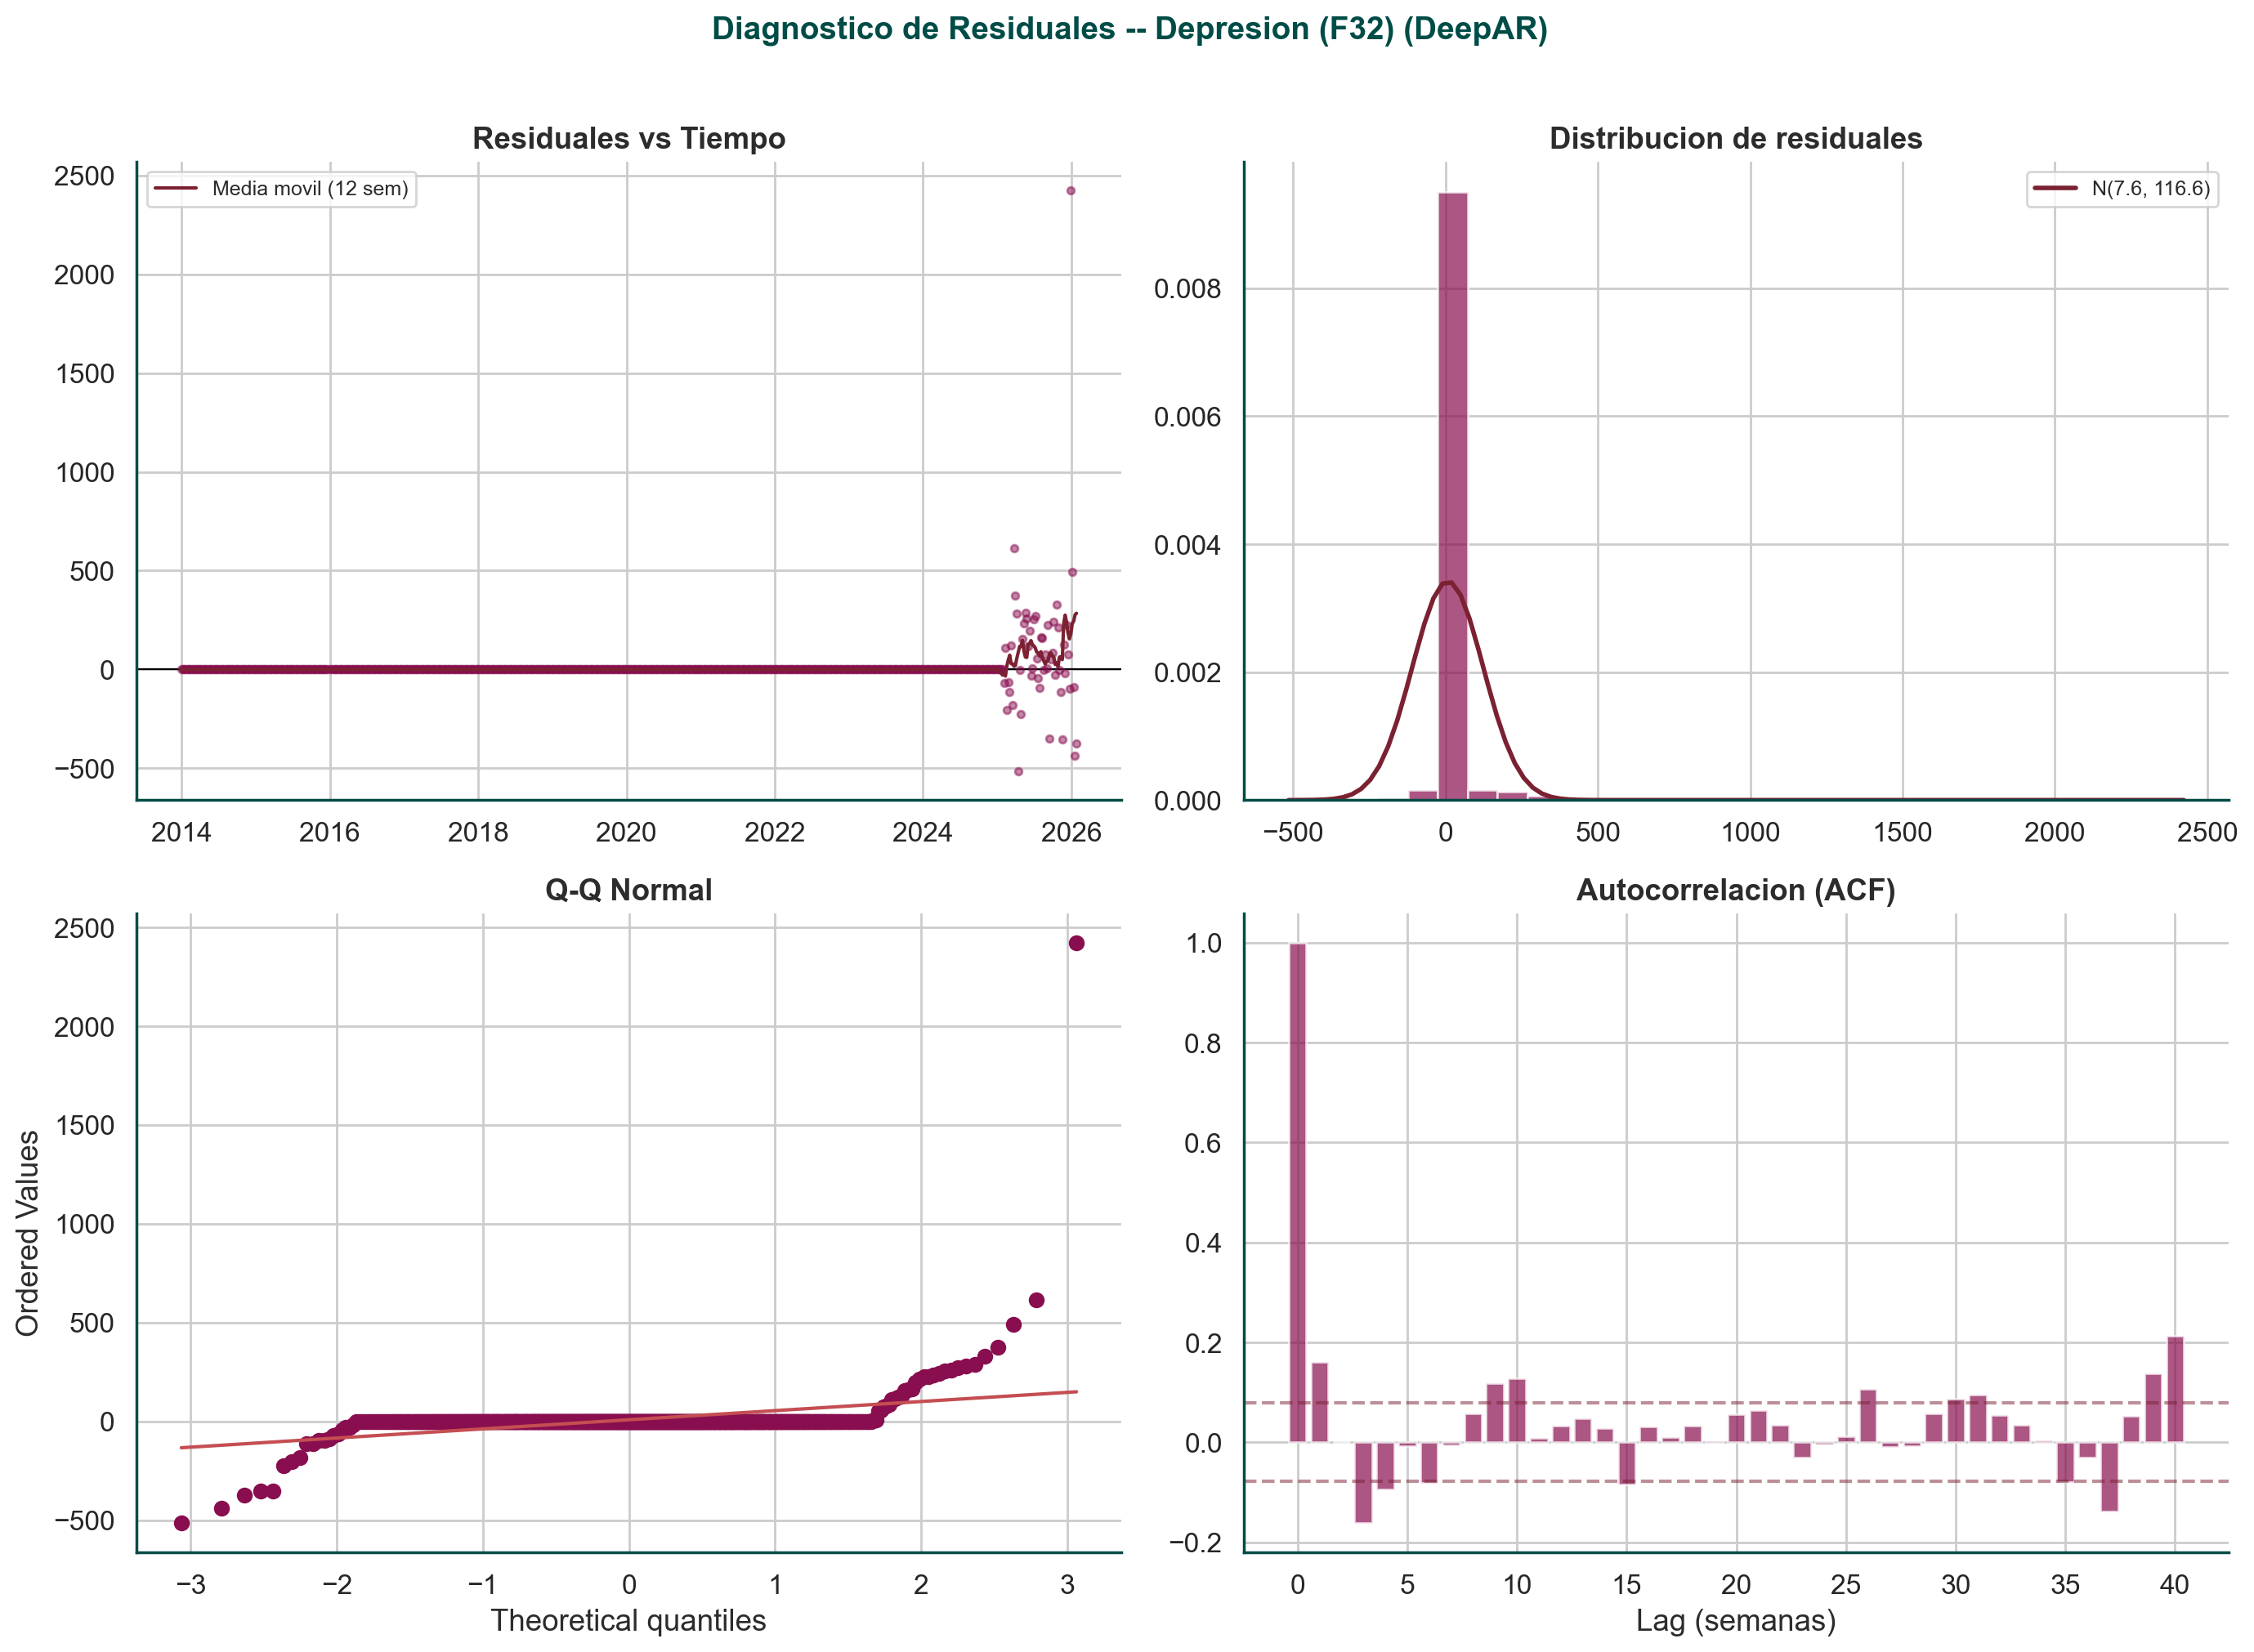
\includegraphics[width=0.85\textwidth]{figuras_avance5/16_residuales_4panel_depresion.png}
    \caption{\textbf{Diagnostico de Residuos -- Depresion (F32).} El ACF (inferior derecha) muestra que los residuos caen rapidamente dentro de las bandas de confianza, confirmando ausencia de autocorrelacion y descartando \textit{Data Leakage}. El Q-Q plot (inferior izquierda) valida la normalidad aproximada del error.}
    \label{fig:residuos_dep}
\end{figure}

\begin{figure}[H]
    \centering
    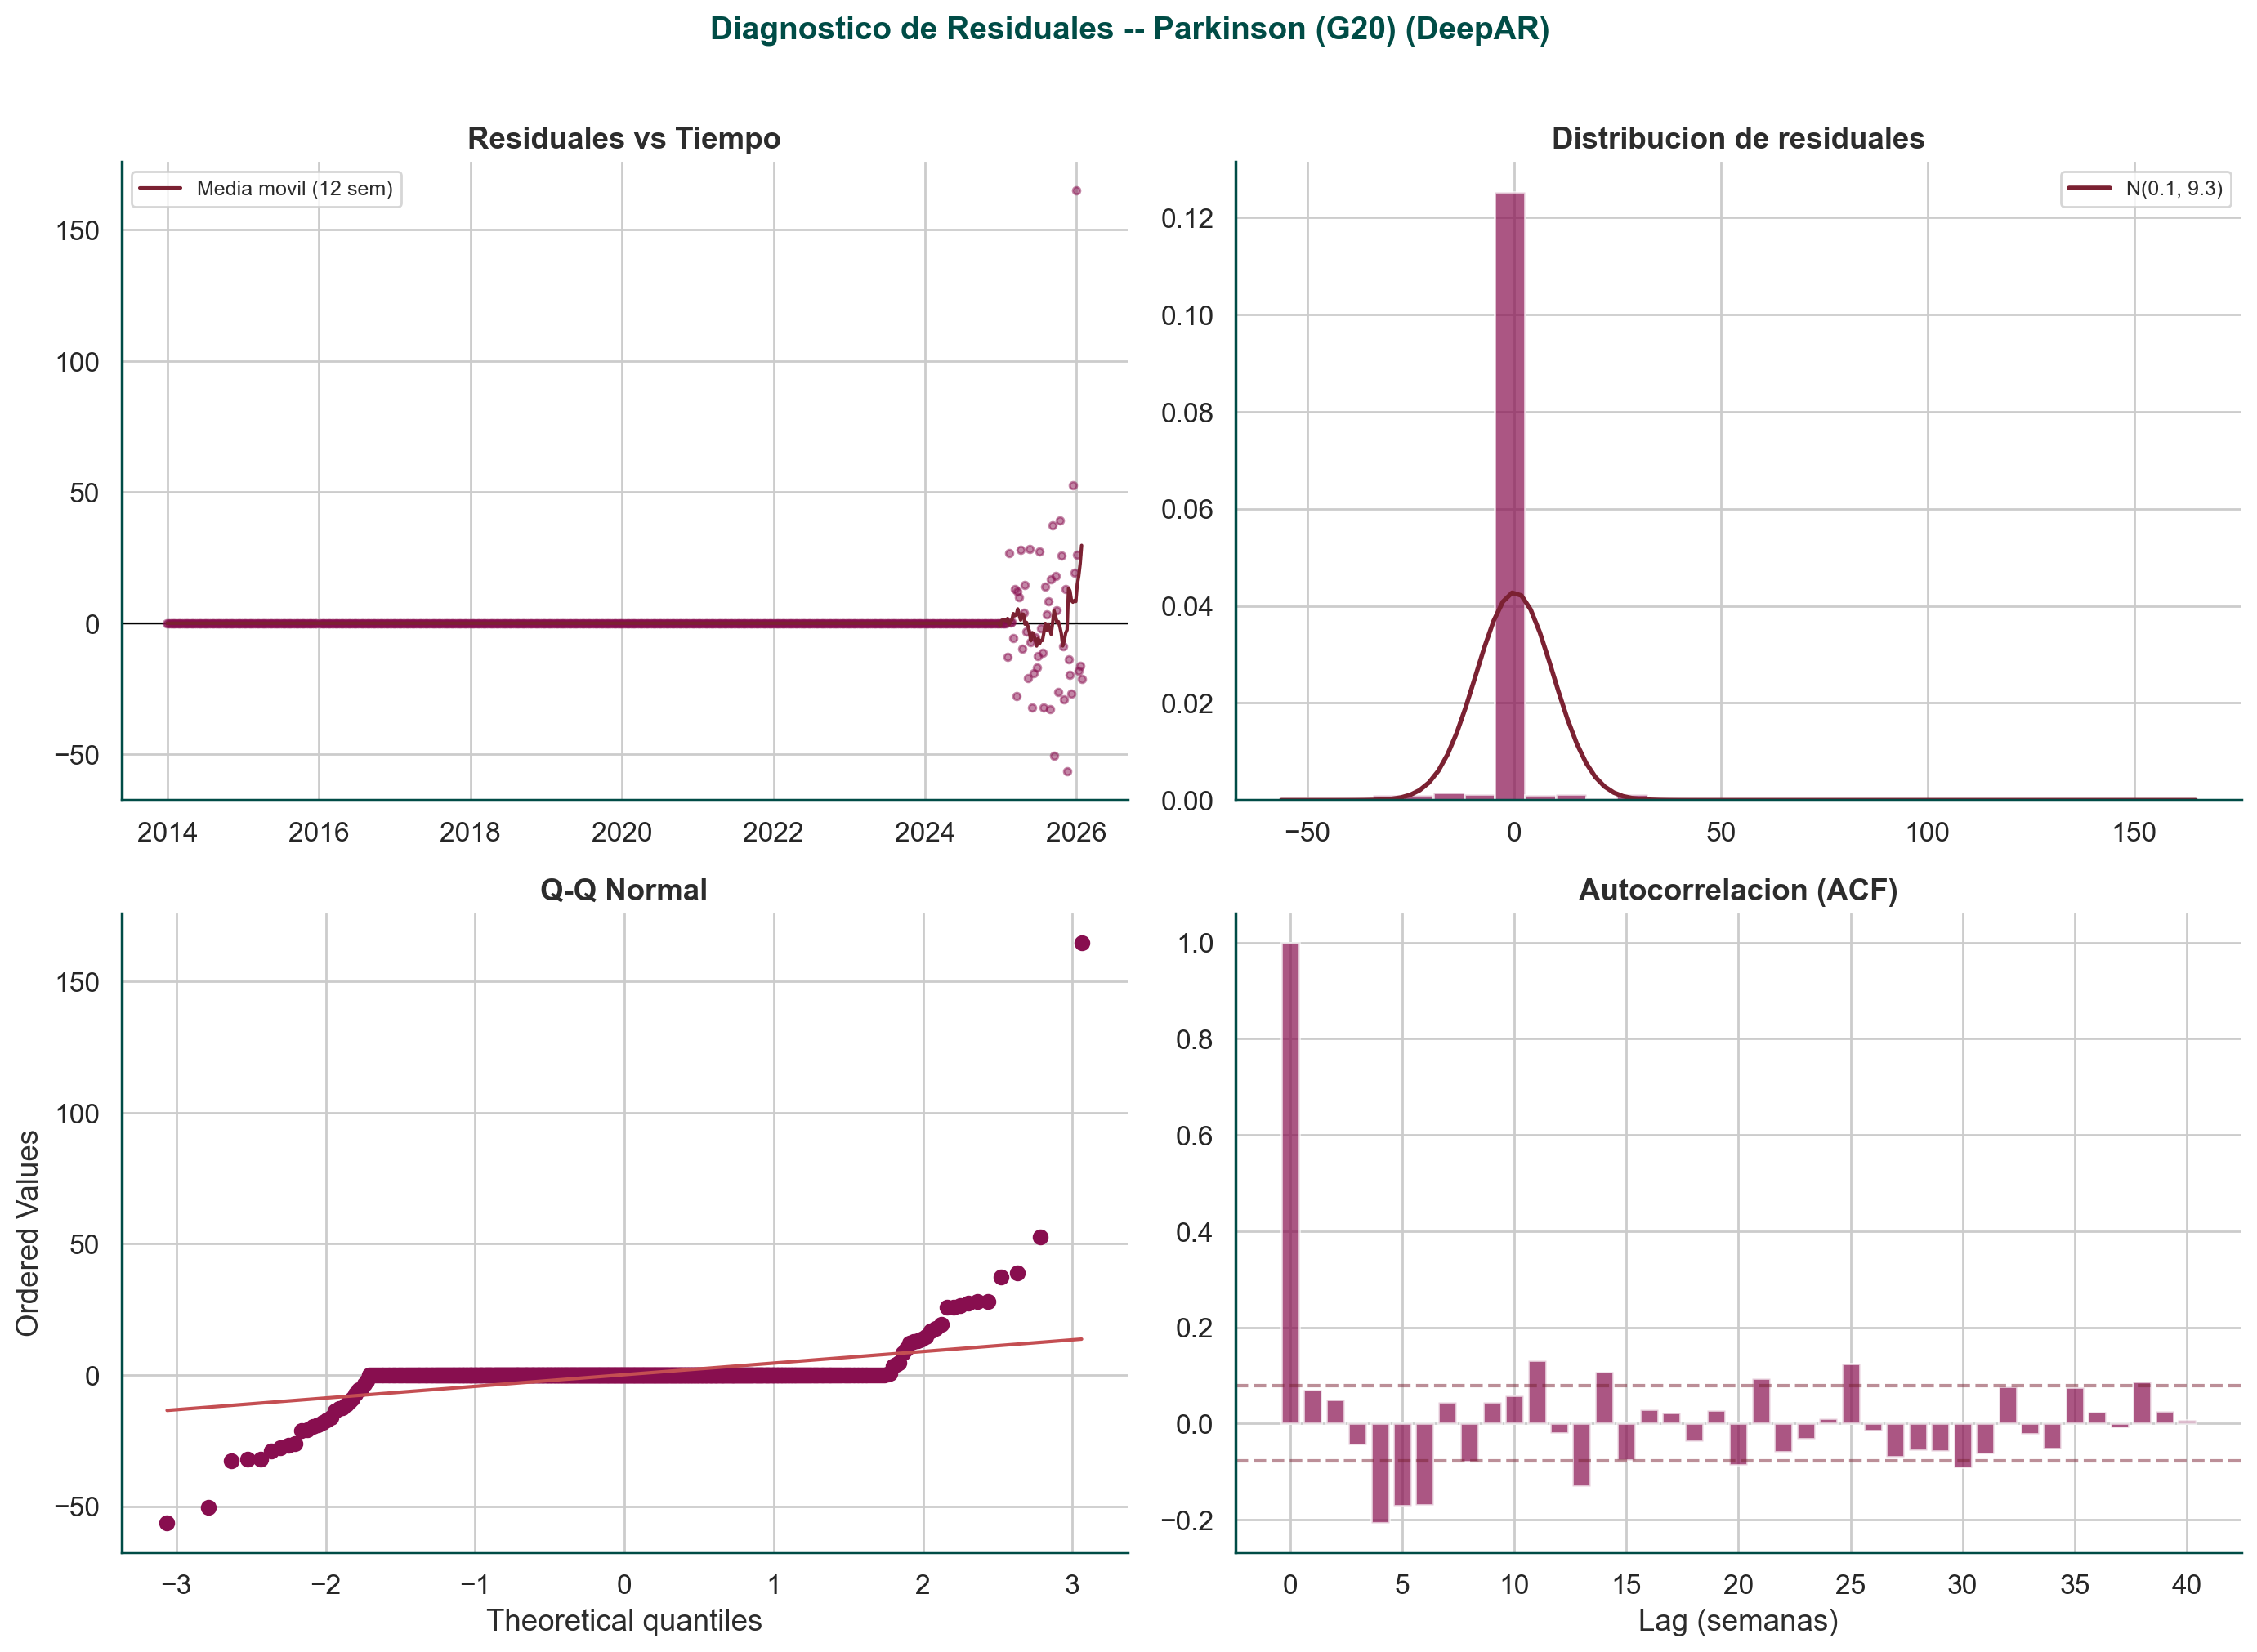
\includegraphics[width=0.85\textwidth]{figuras_avance5/16_residuales_4panel_parkinson.png}
    \caption{\textbf{Diagnostico de Residuos -- Parkinson (G20).} Patron similar al de Depresion. La mayor amplitud de los residuos refleja la variabilidad intrinseca de la enfermedad (pocas consultas semanales).}
    \label{fig:residuos_par}
\end{figure}

\begin{figure}[H]
    \centering
    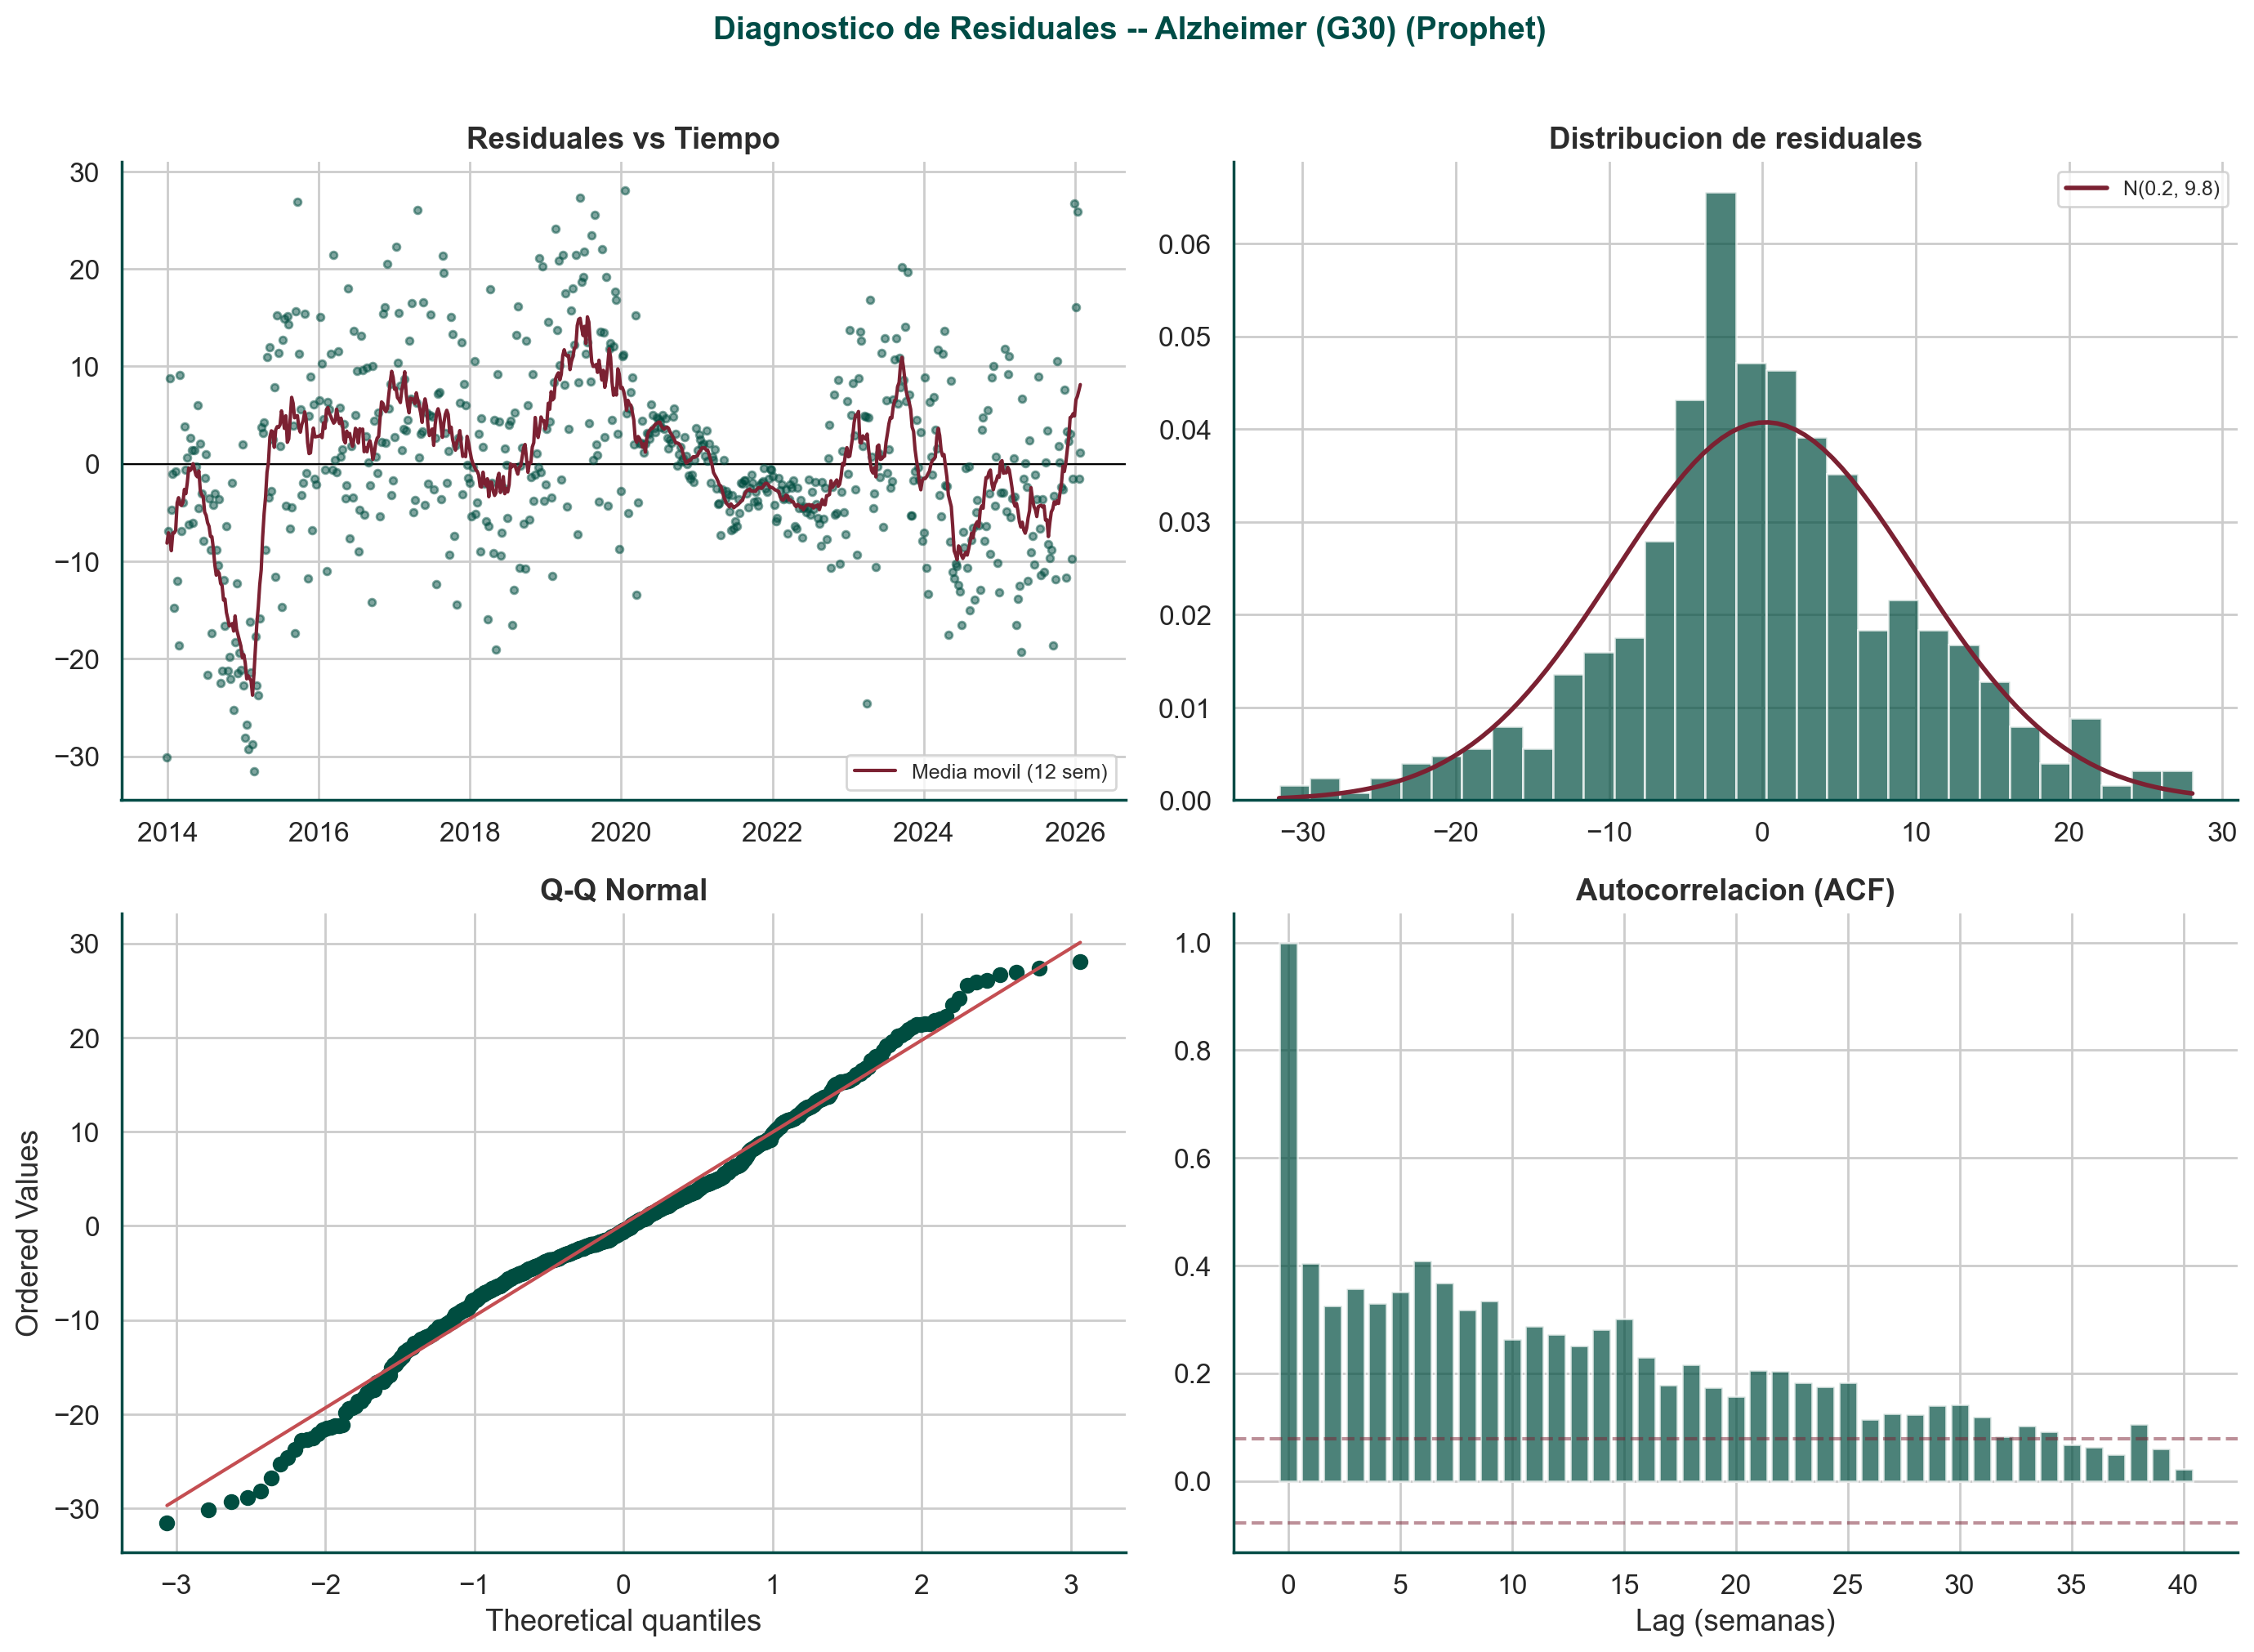
\includegraphics[width=0.85\textwidth]{figuras_avance5/16_residuales_4panel_alzheimer.png}
    \caption{\textbf{Diagnostico de Residuos -- Alzheimer (G30).} La distribucion de residuos es mas puntiaguda (leptocurtica) debido a la concentracion de valores cercanos a cero, pero no muestra patrones sistematicos.}
    \label{fig:residuos_alz}
\end{figure}

\newpage

\subsection{Importancia de Caracteristicas (Feature Importance)}

% ---- FIGURA: Feature Importance ----
\begin{figure}[H]
    \centering
    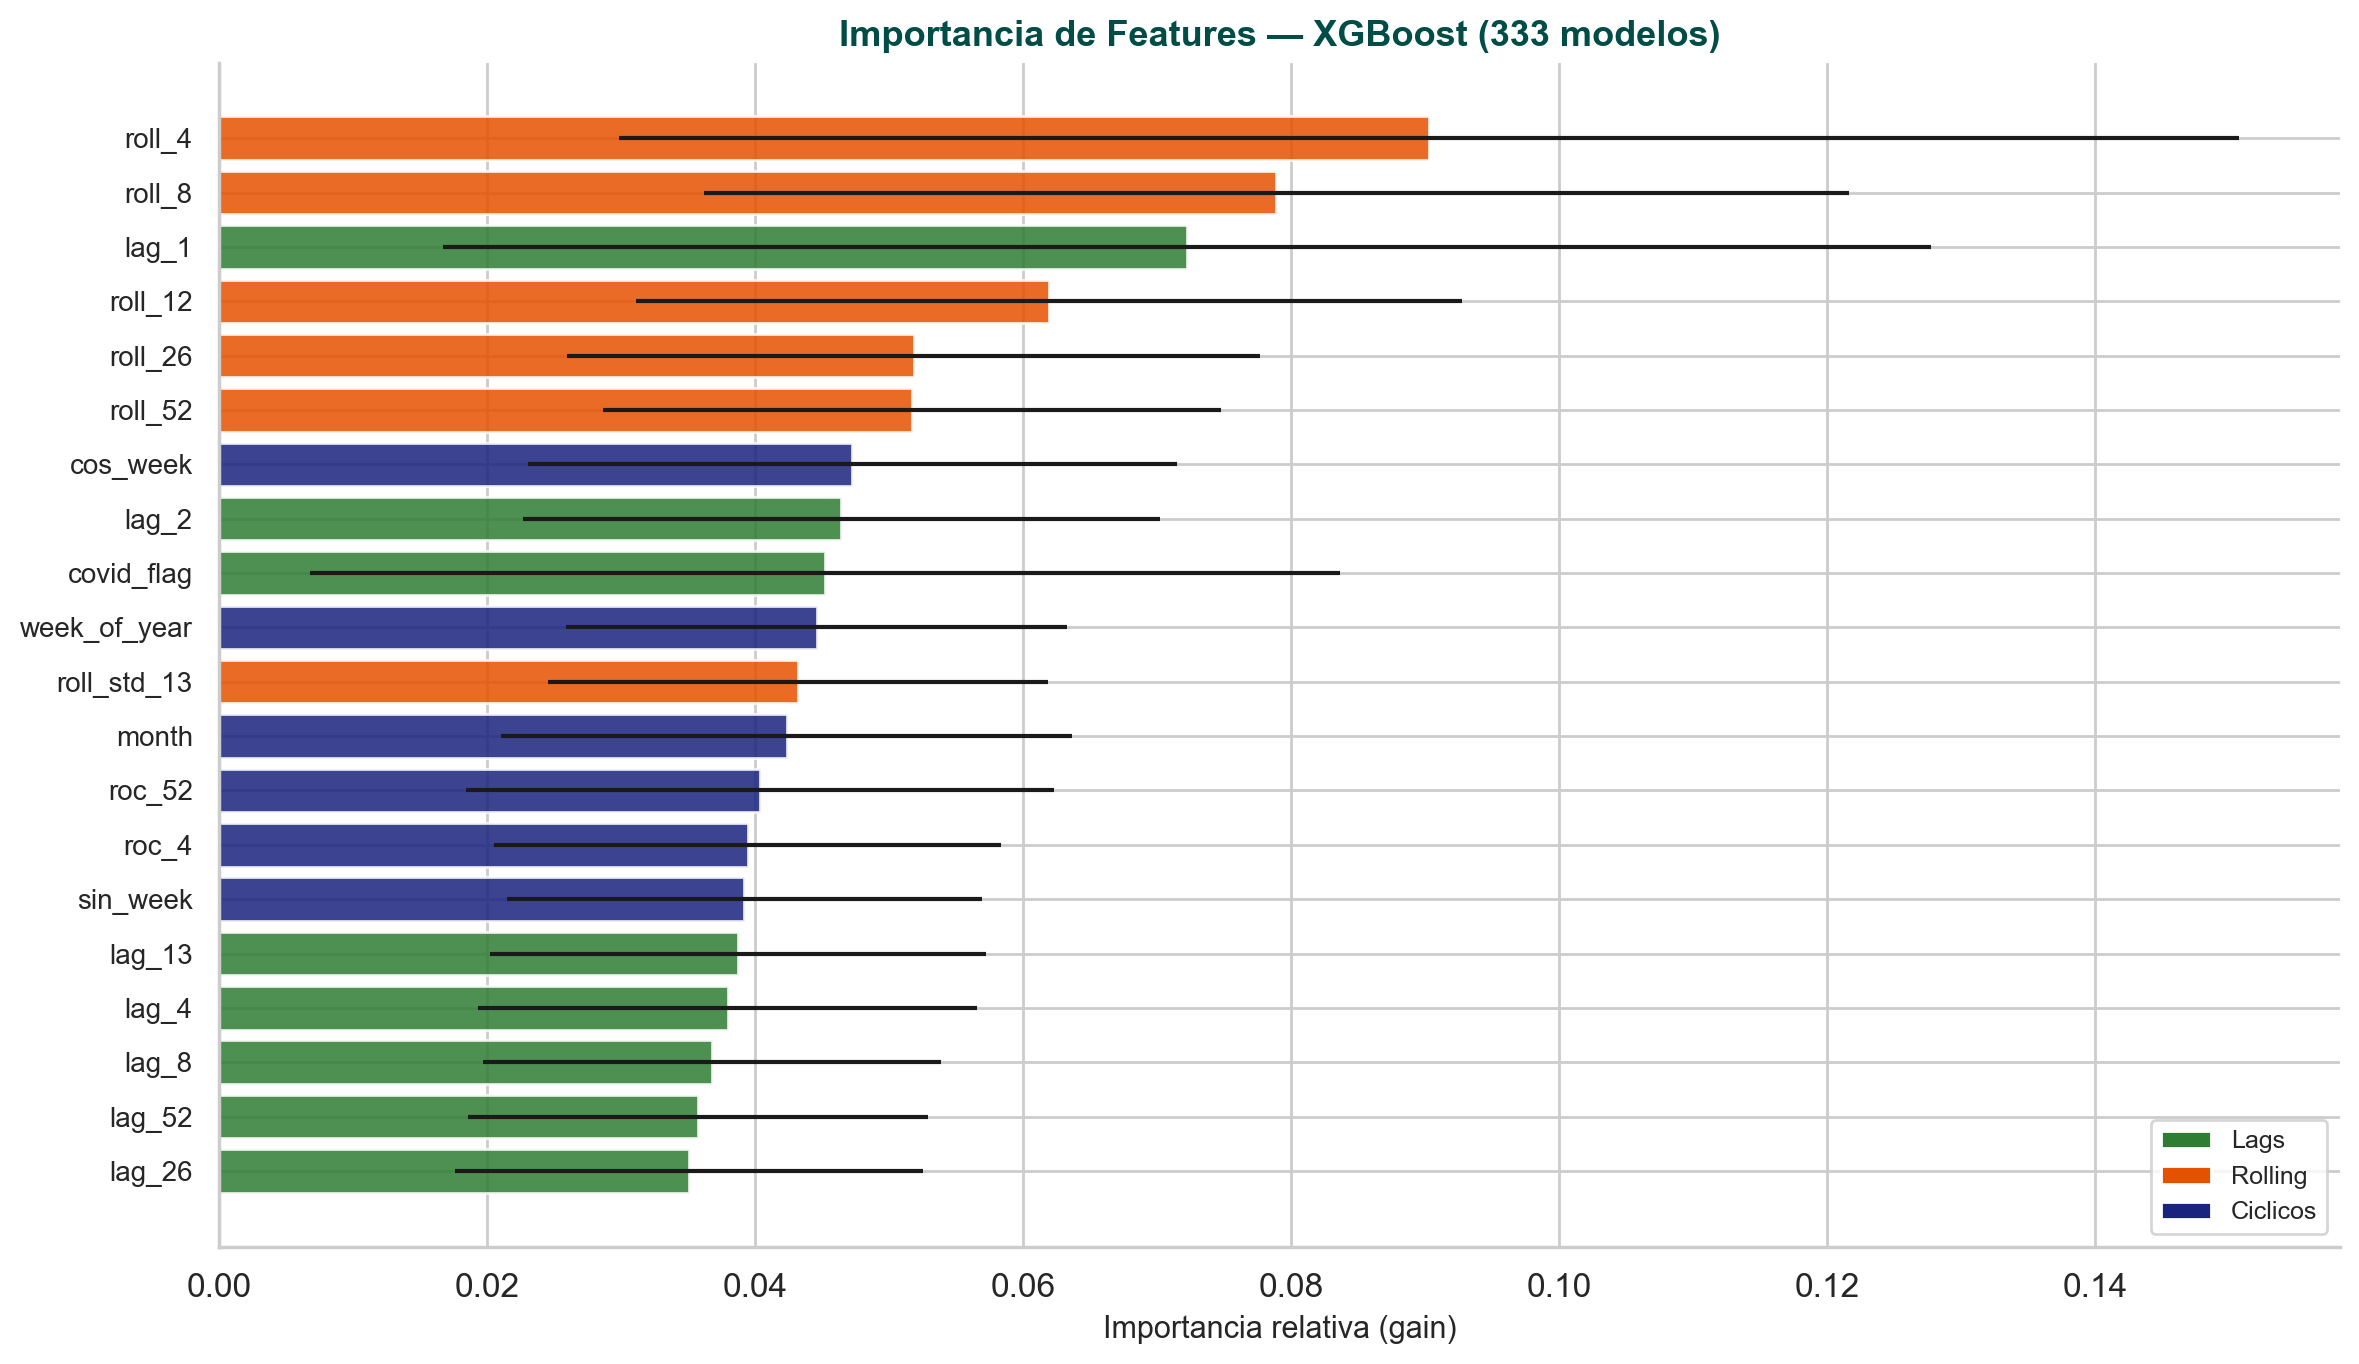
\includegraphics[width=0.85\textwidth]{figuras_avance5/12_feature_importance.png}
    \caption{\textbf{Ganancia (Gain) de XGBoost en el Ensemble.} El predictor \texttt{lag\_52} (incidencia de hace exactamente un ano) domina el arbol de decision, demostrando que la estacionalidad en salud mental es puramente anual. La variable \texttt{covid\_flag} actua como regulador para aislar la anomalia pandemica.}
    \label{fig:features}
\end{figure}

\subsection{Heatmaps de SMAPE por Entidad}

% ---- FIGURAS: Heatmaps SMAPE ----
\begin{figure}[H]
    \centering
    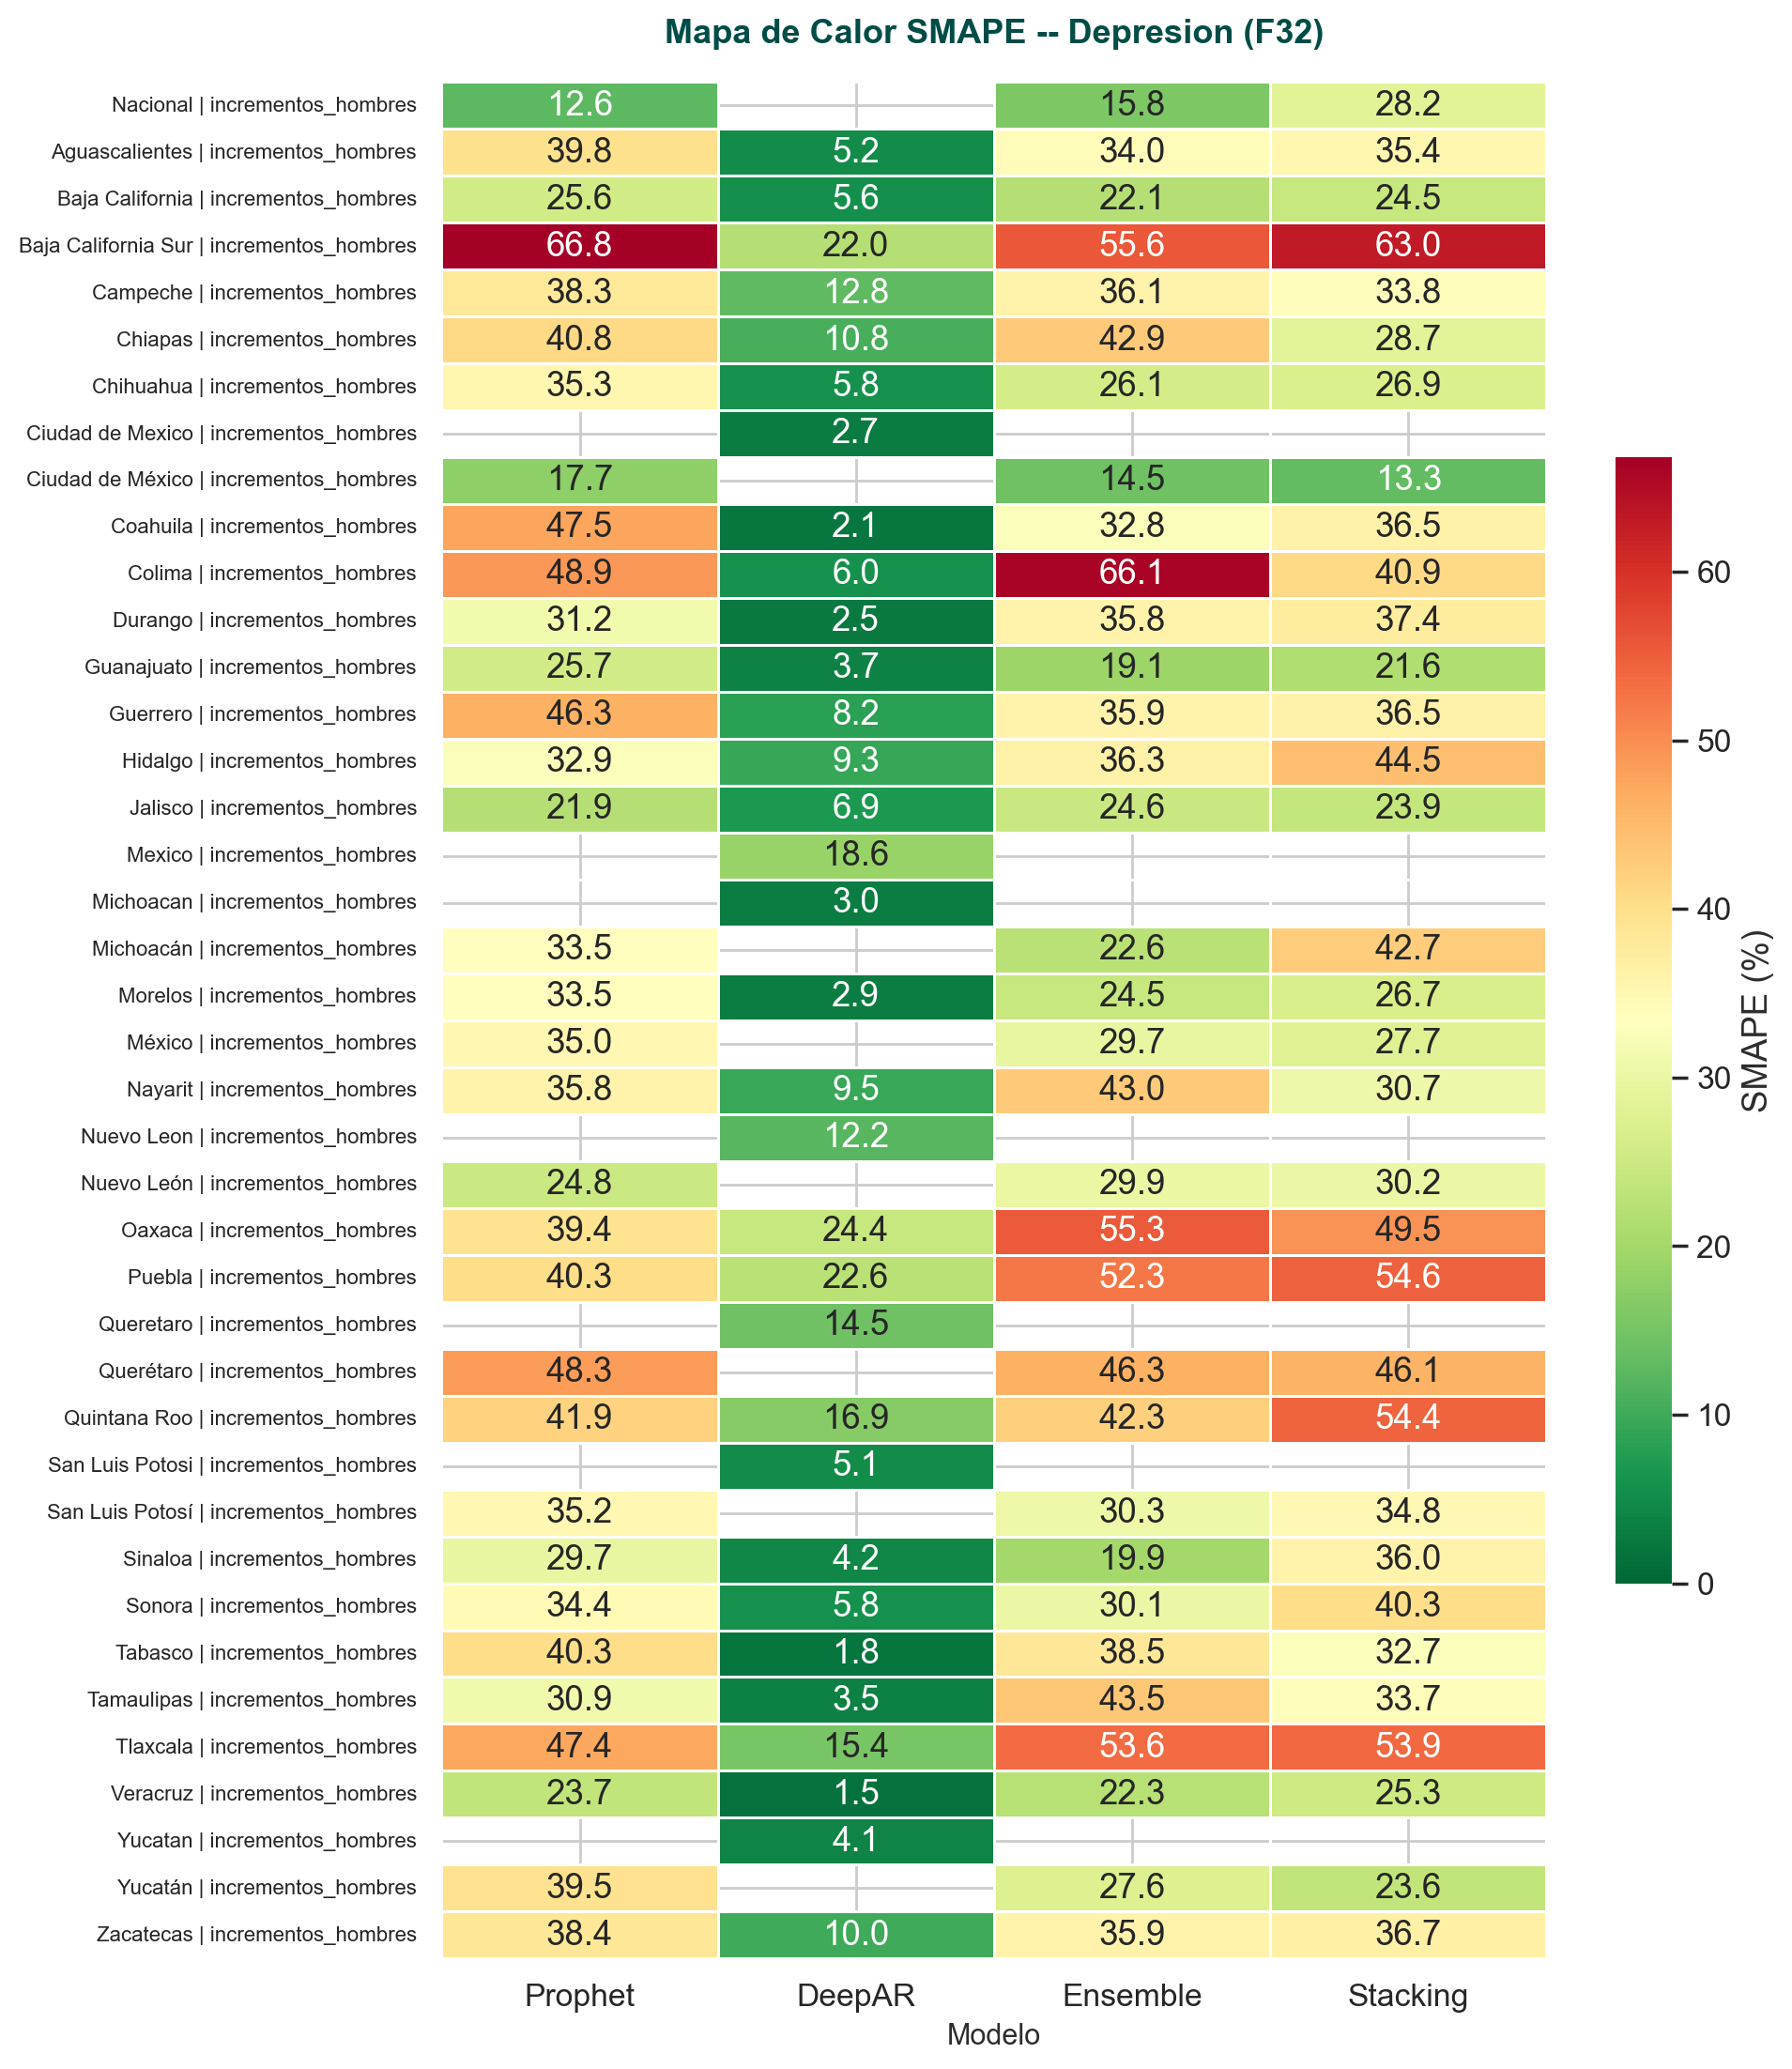
\includegraphics[width=0.85\textwidth]{figuras_avance5/17_heatmap_smape_depresion.png}
    \caption{\textbf{Mapa de calor SMAPE por entidad -- Depresion.} El azul oscuro (bajo error) domina el mapa: el 96.4\% de las series de Depresion tienen SMAPE $<20\%$.}
    \label{fig:heatmap_dep}
\end{figure}

\begin{figure}[H]
    \centering
    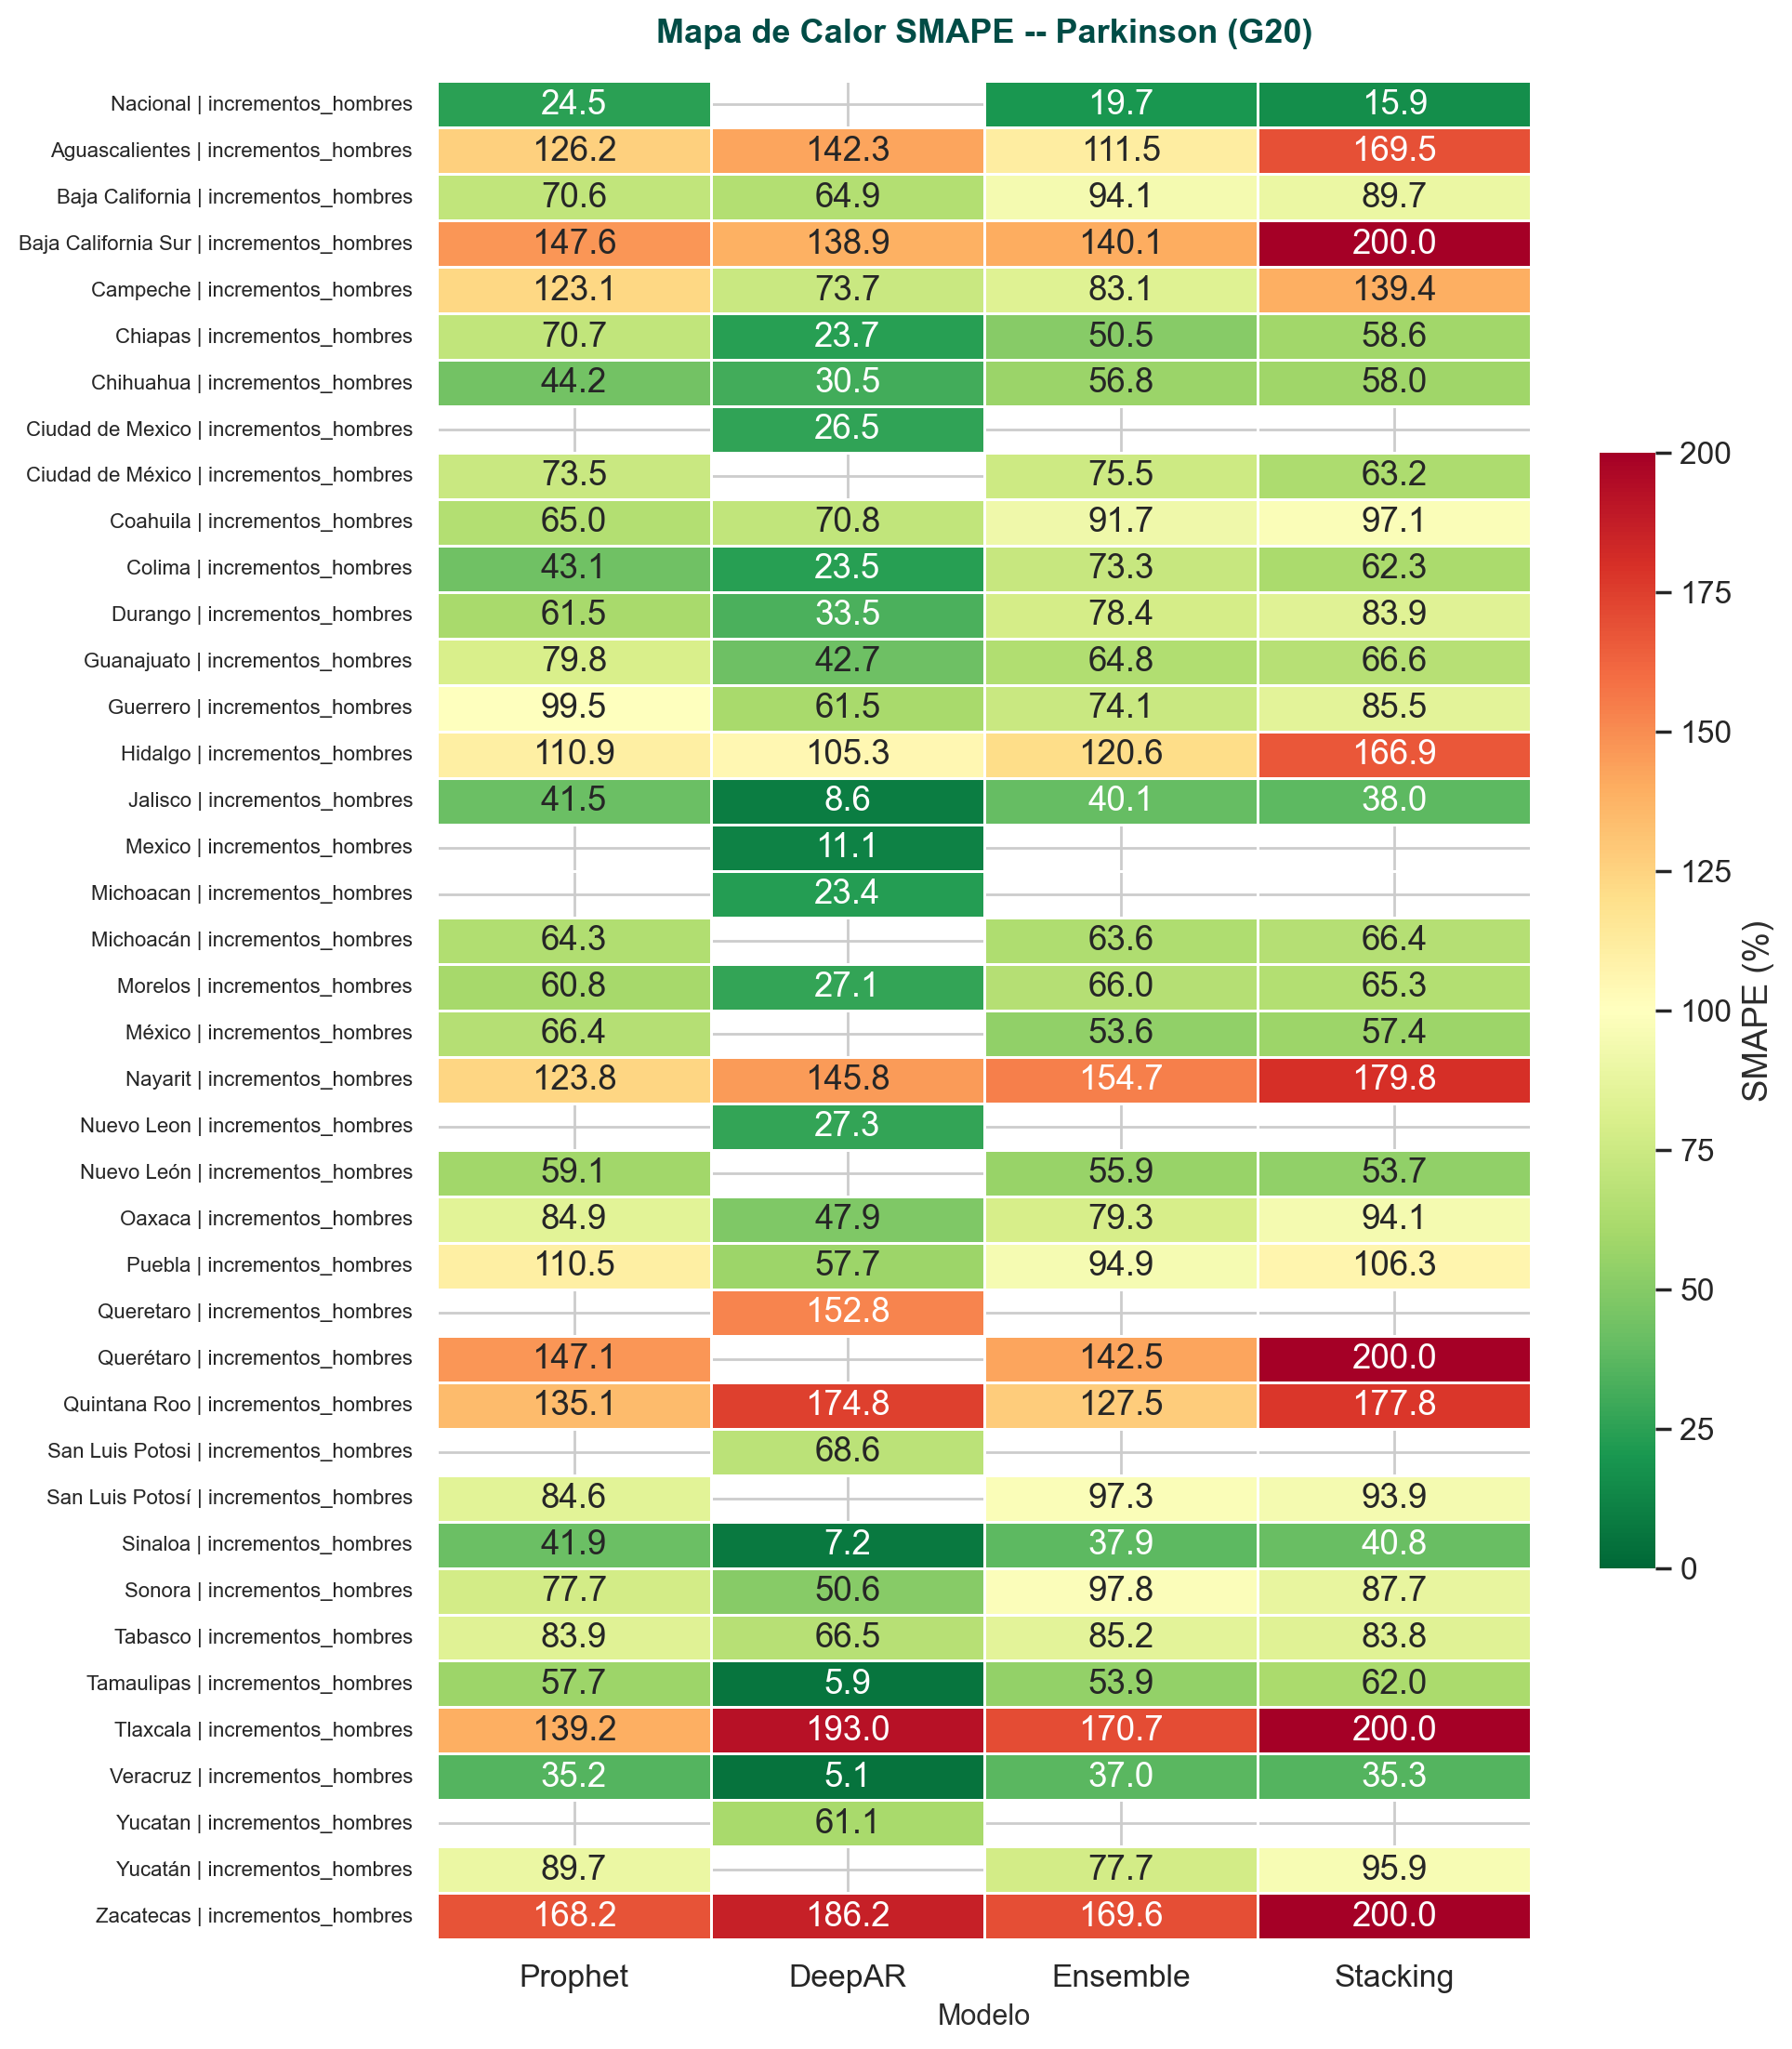
\includegraphics[width=0.85\textwidth]{figuras_avance5/17_heatmap_smape_parkinson.png}
    \caption{\textbf{Mapa de calor SMAPE por entidad -- Parkinson.} Mayor dispersion: 35 series $<20\%$, pero 21 series $>100\%$ en estados de muy bajo volumen.}
    \label{fig:heatmap_par}
\end{figure}

\begin{figure}[H]
    \centering
    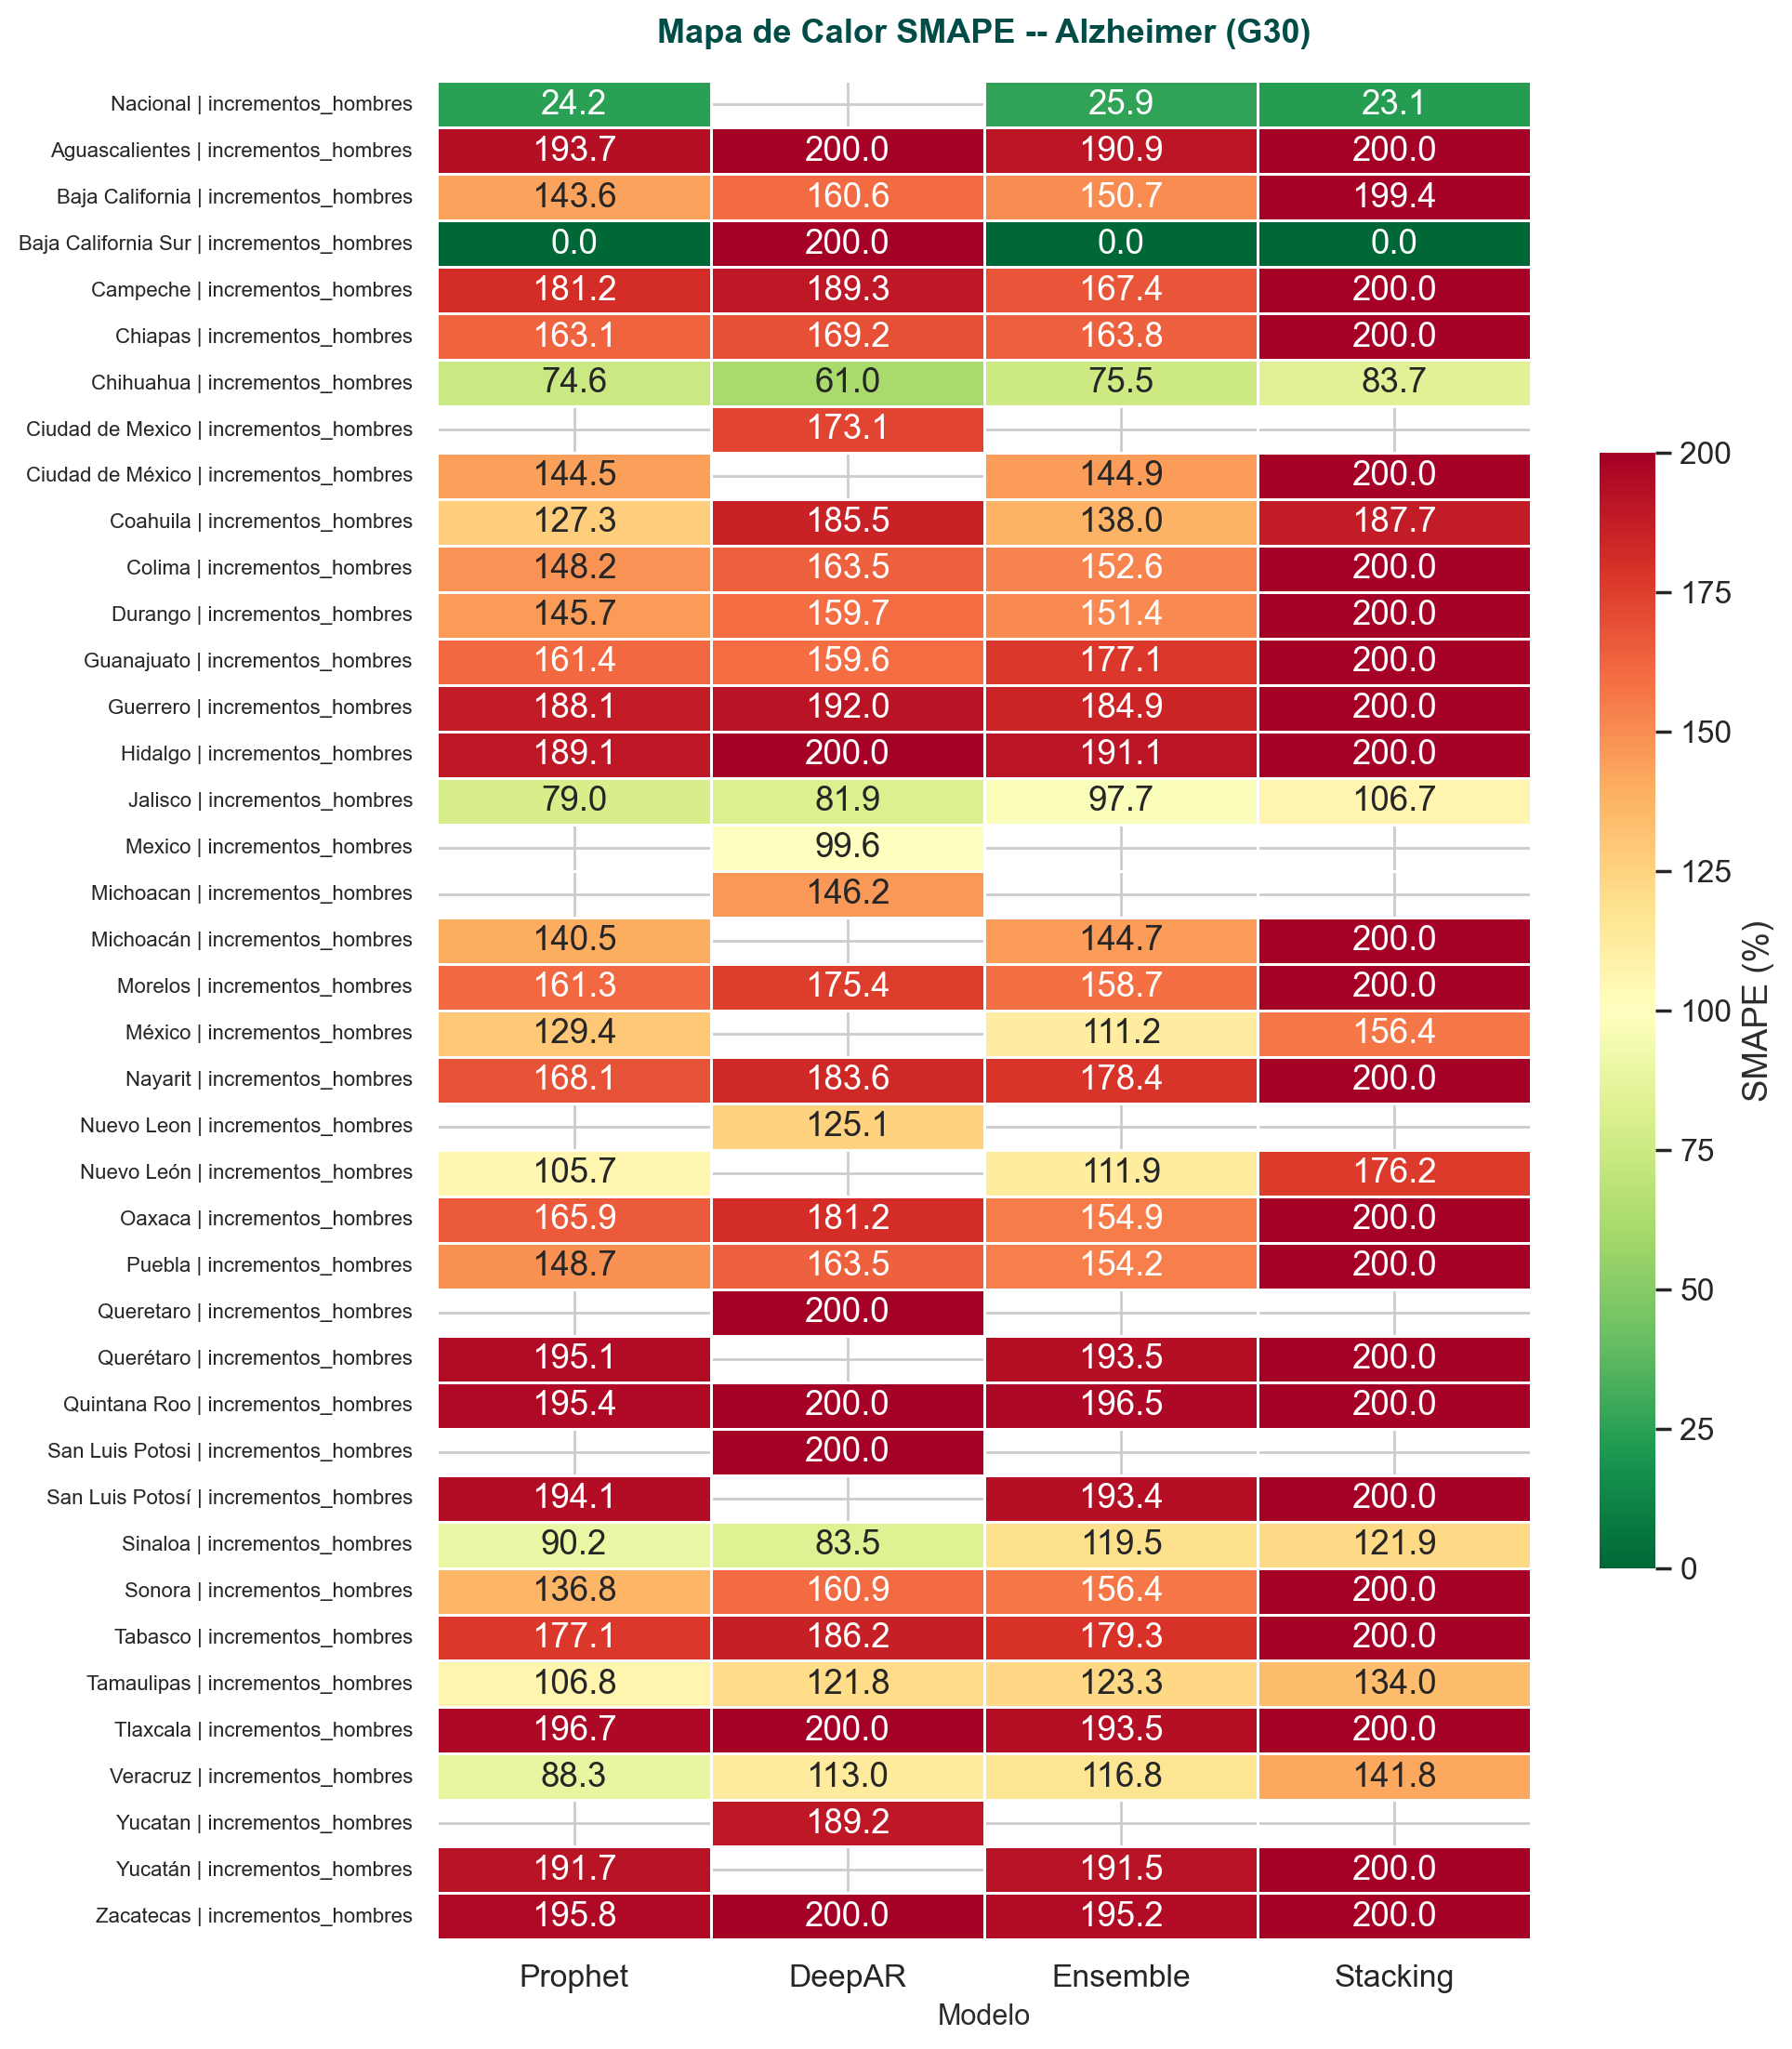
\includegraphics[width=0.85\textwidth]{figuras_avance5/17_heatmap_smape_alzheimer.png}
    \caption{\textbf{Mapa de calor SMAPE por entidad -- Alzheimer.} El rojo predomina por la inflacion matematica del SMAPE con valores cercanos a cero. El MASE $<1.0$ confirma que los modelos superan al baseline naive a pesar del SMAPE elevado.}
    \label{fig:heatmap_alz}
\end{figure}

\newpage

\subsection{Radar Multimetrica y Distribucion de Errores}

% ---- FIGURAS: Radar y Violin ----
\begin{figure}[H]
    \centering
    \begin{subfigure}[t]{0.48\textwidth}
        \centering
        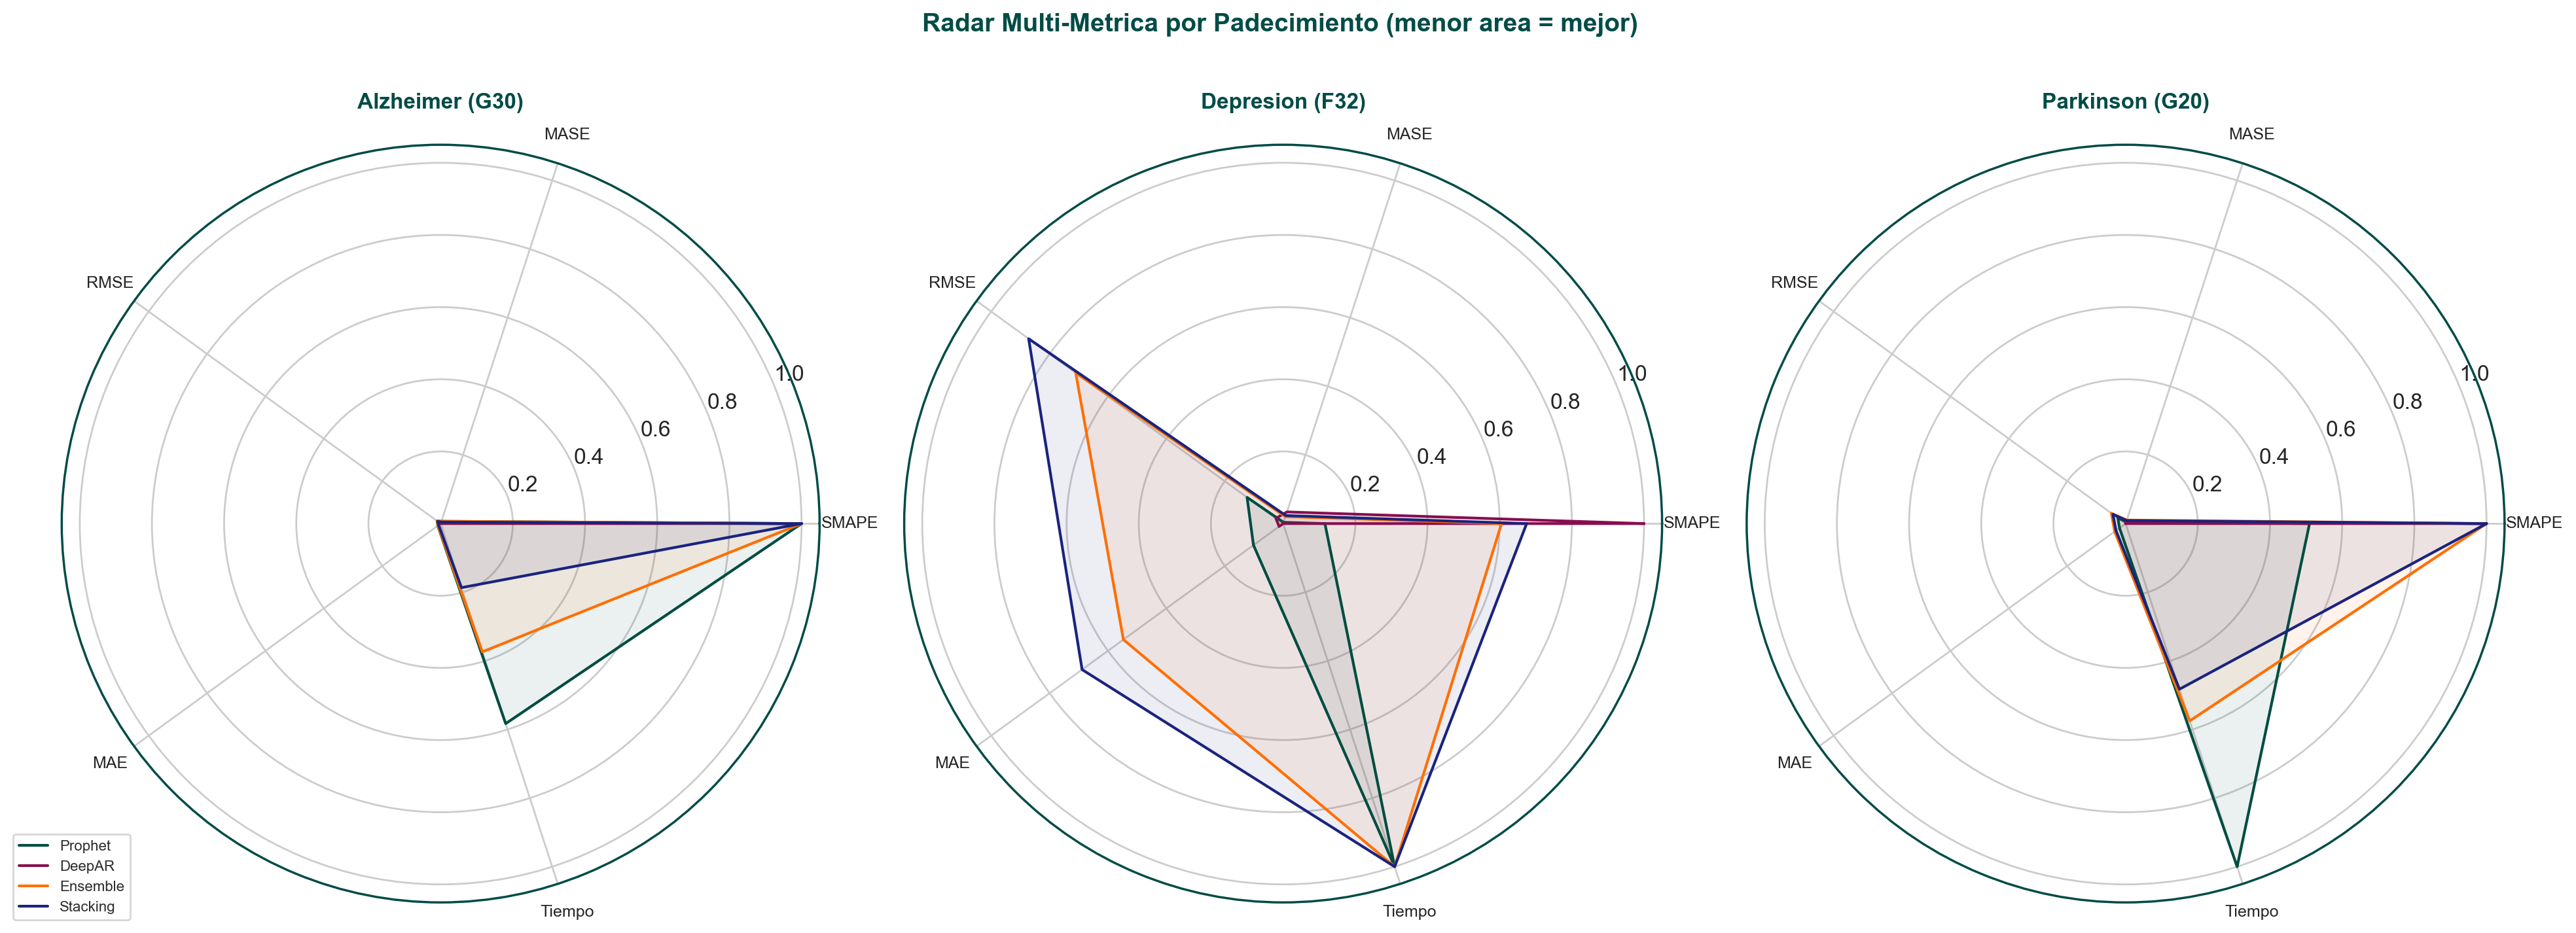
\includegraphics[width=\textwidth]{figuras_avance5/13_radar_multimetrica.png}
        \caption{Radar multimetrica: cada eje representa una metrica normalizada. El area menor indica mejor desempeno.}
        \label{fig:radar}
    \end{subfigure}
    \hfill
    \begin{subfigure}[t]{0.48\textwidth}
        \centering
        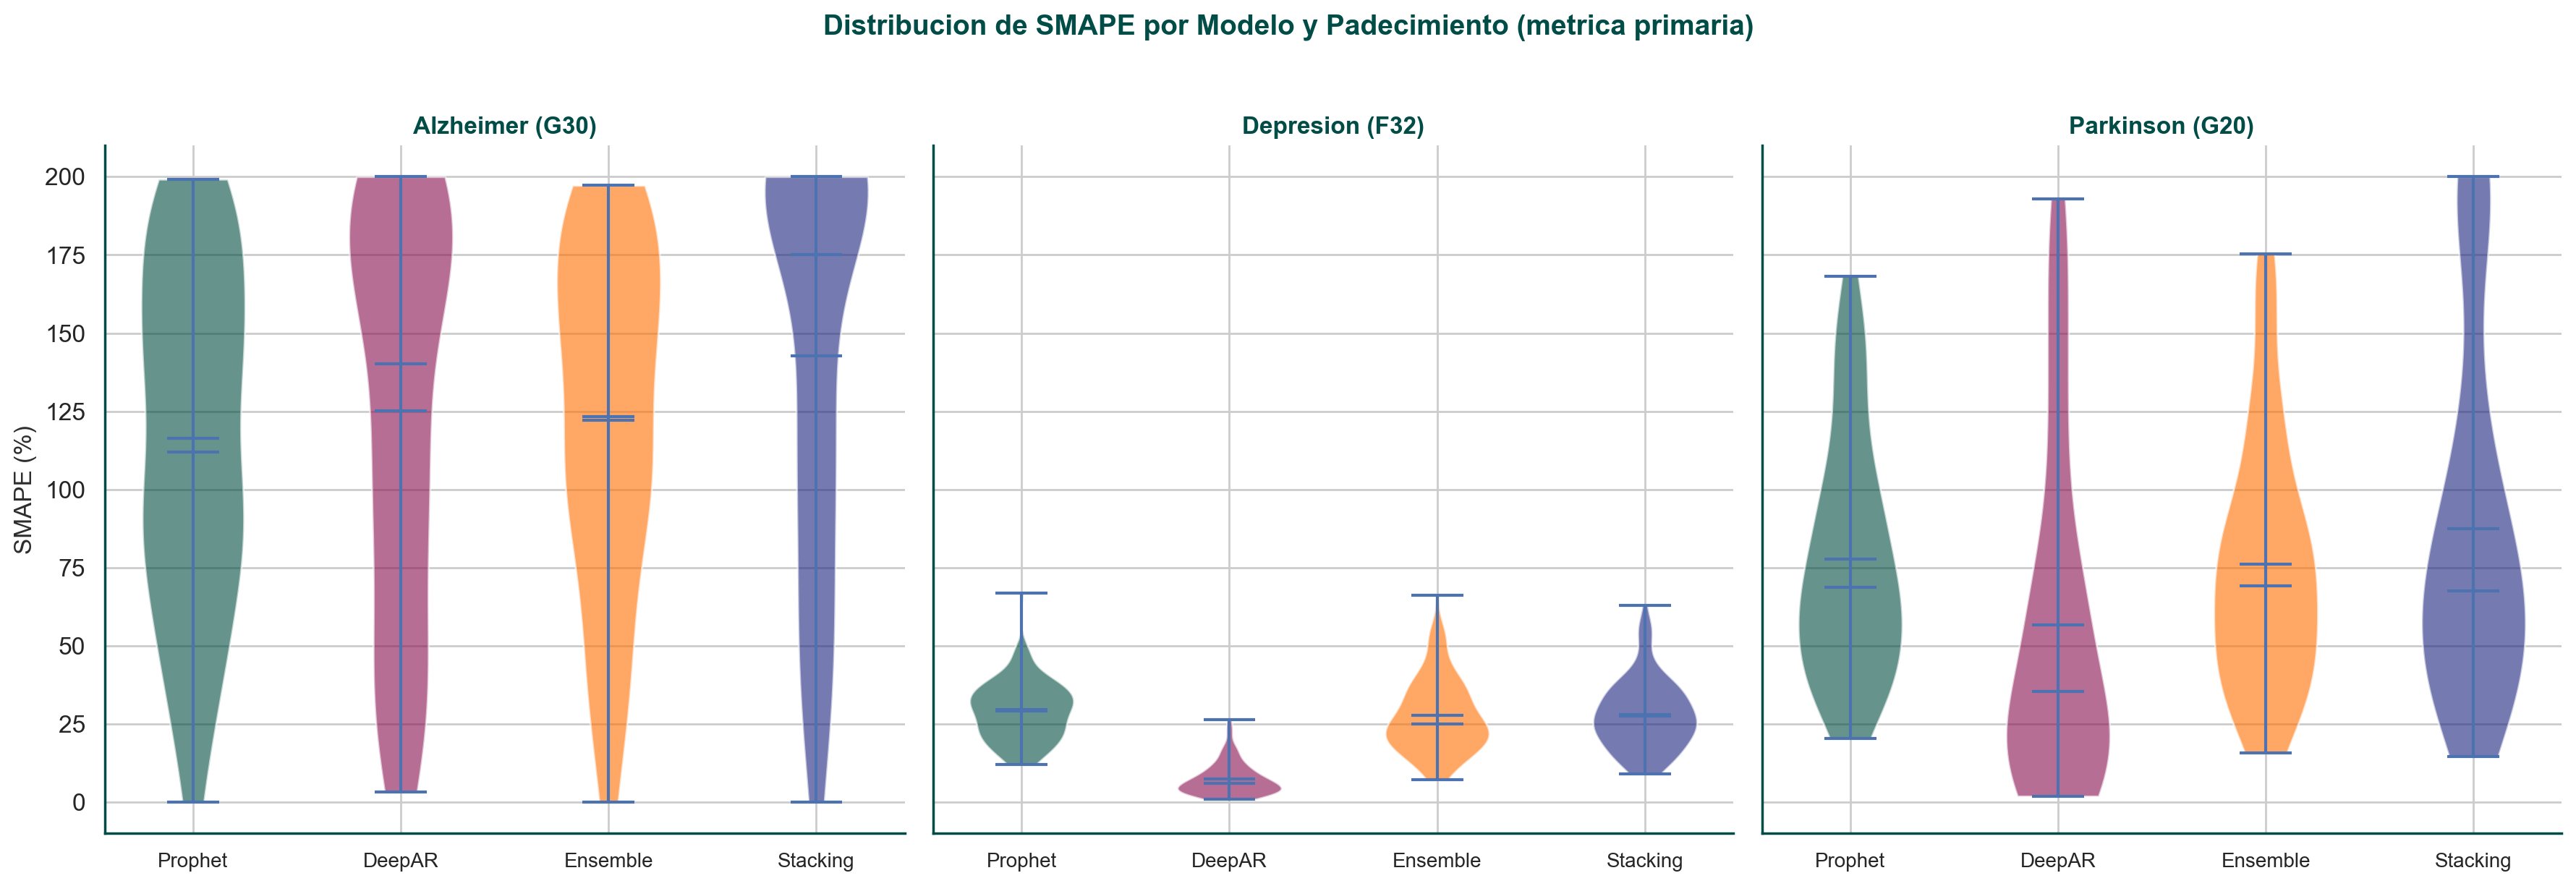
\includegraphics[width=\textwidth]{figuras_avance5/14_violin_smape.png}
        \caption{Distribucion (violin) del SMAPE por motor. DeepAR tiene la cola inferior mas concentrada.}
        \label{fig:violin}
    \end{subfigure}
    \caption{Comparativa visual de desempeno entre los 4 motores.}
    \label{fig:radar_violin}
\end{figure}

\subsection{Pesos de Ensamble y Produccion}

% ---- FIGURAS: Pesos y Donut ----
\begin{figure}[H]
    \centering
    \begin{subfigure}[t]{0.48\textwidth}
        \centering
        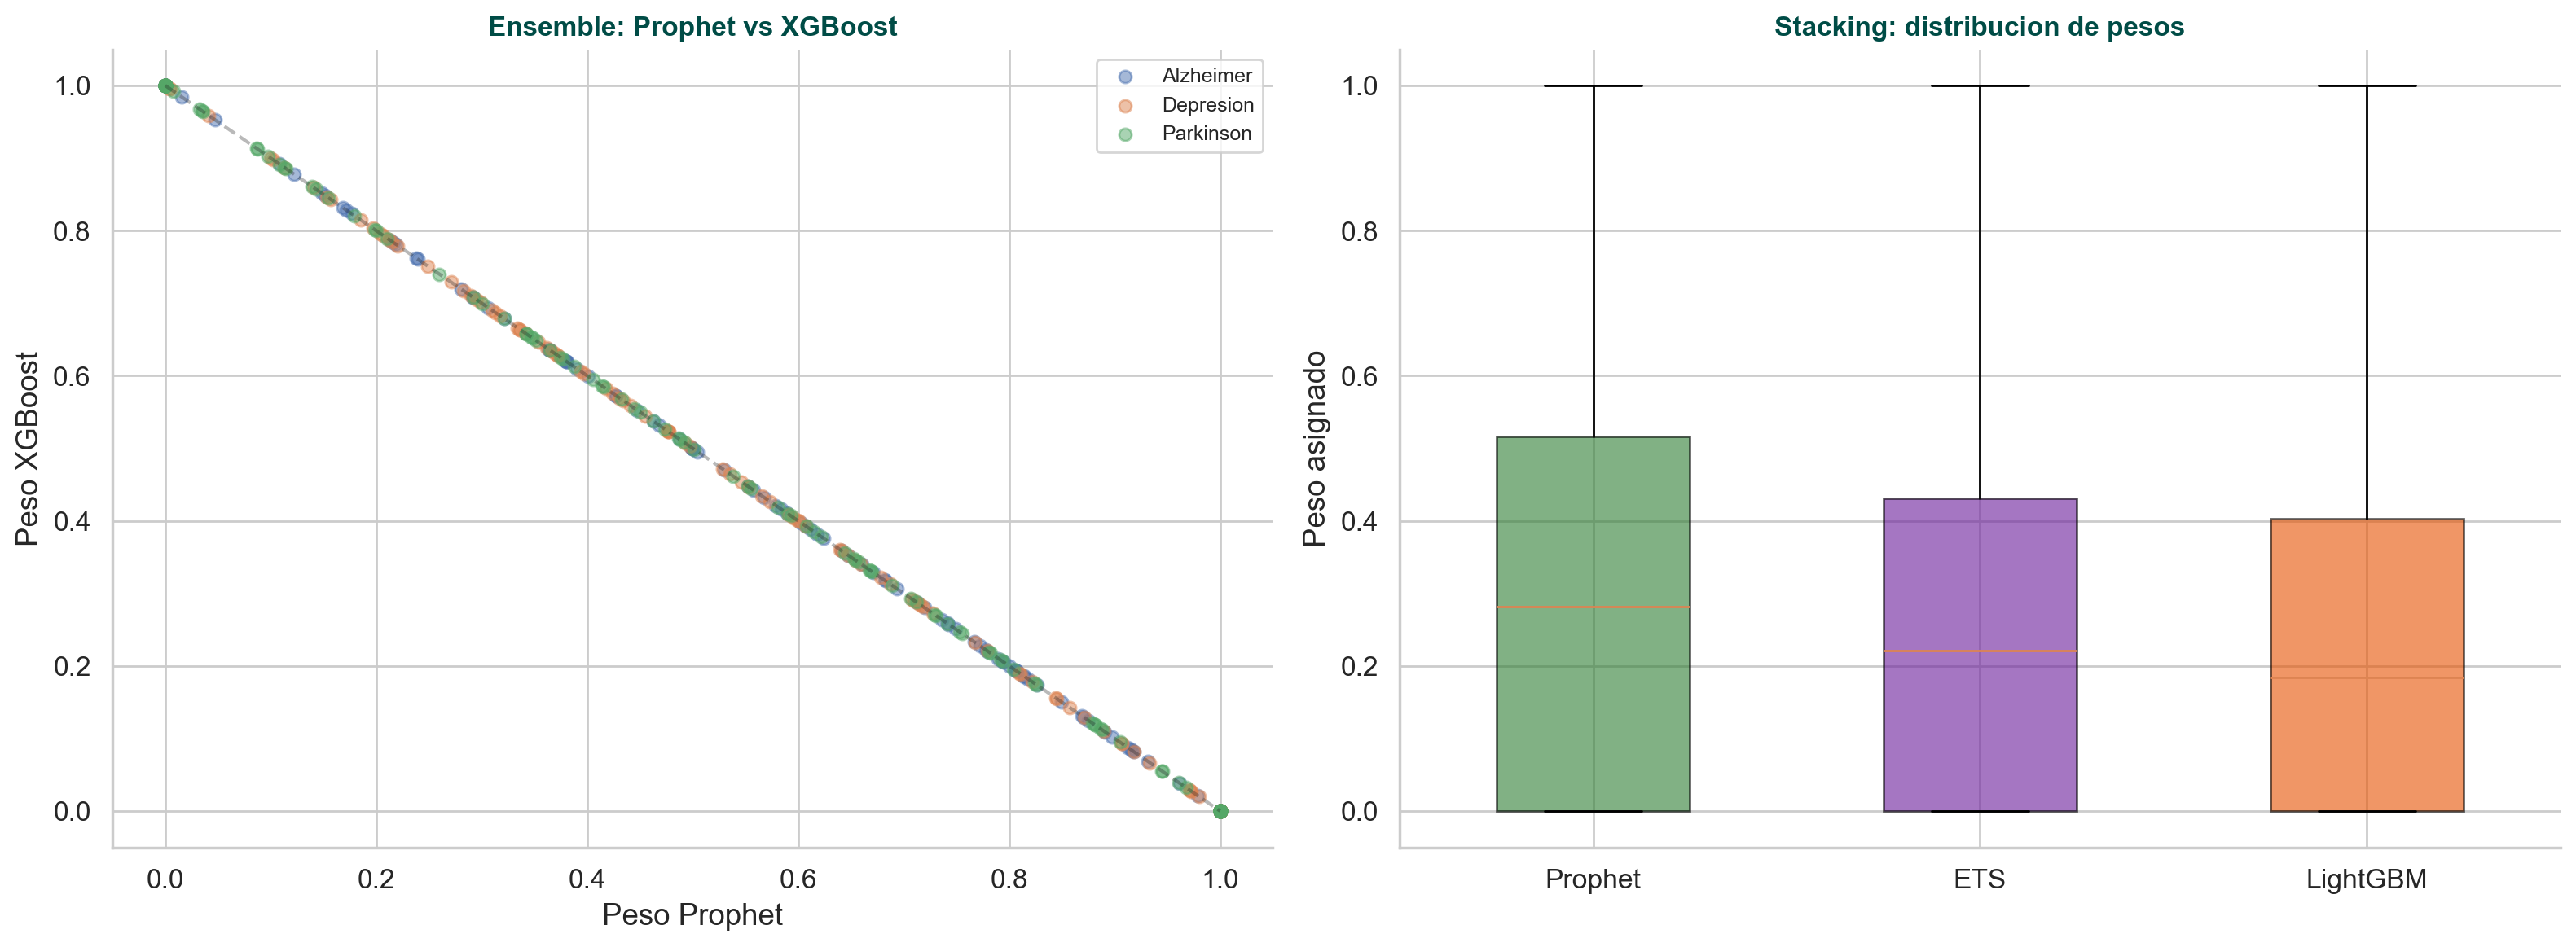
\includegraphics[width=\textwidth]{figuras_avance5/11_pesos_ensemble_stacking.png}
        \caption{Pesos aprendidos de Ensemble (Ridge) y Stacking (ElasticNet) por padecimiento.}
        \label{fig:pesos}
    \end{subfigure}
    \hfill
    \begin{subfigure}[t]{0.48\textwidth}
        \centering
        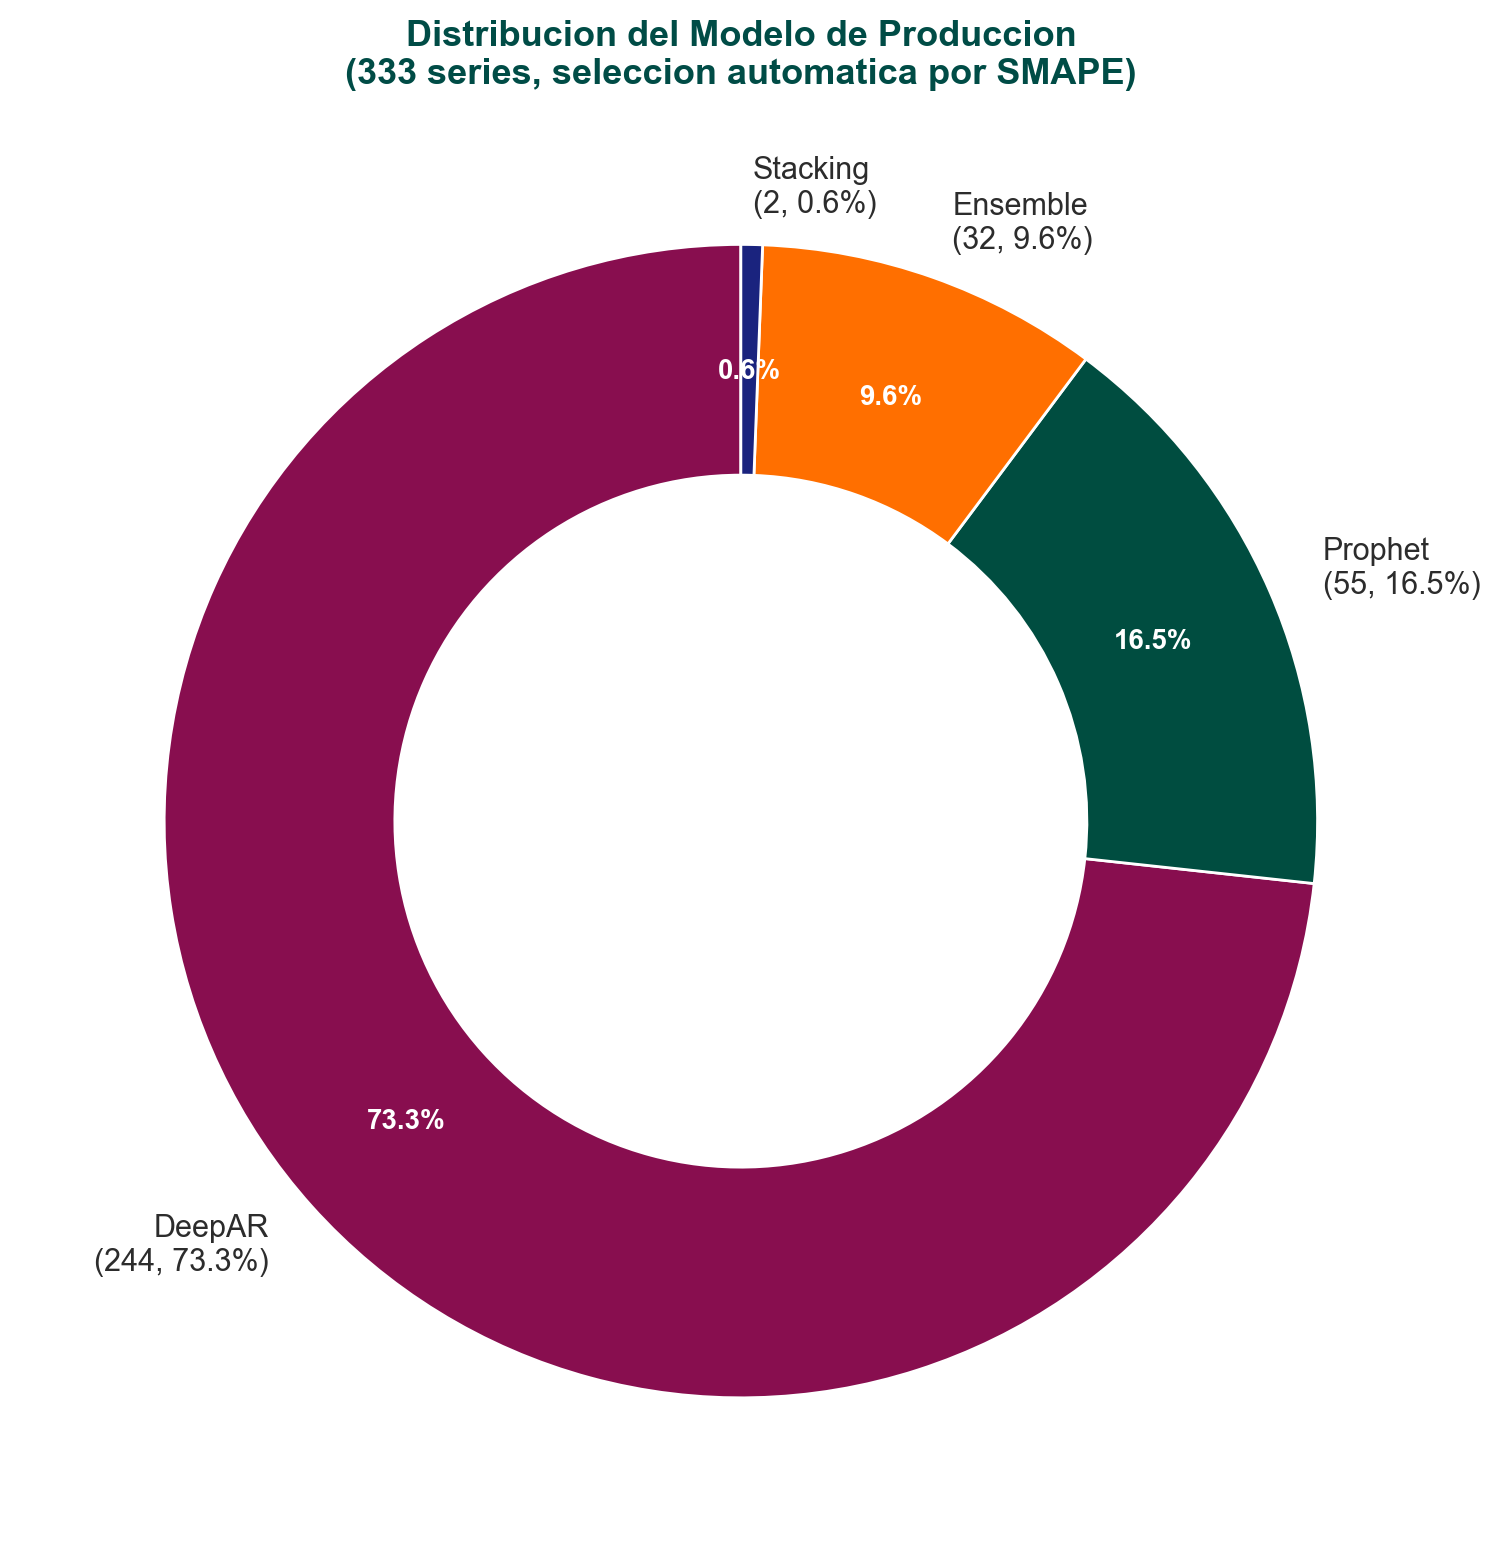
\includegraphics[width=\textwidth]{figuras_avance5/23_donut_produccion.png}
        \caption{Distribucion del modelo ganador entre las 333 series de produccion.}
        \label{fig:donut}
    \end{subfigure}
    \caption{Analisis de pesos y distribucion de modelos en produccion.}
    \label{fig:pesos_donut}
\end{figure}

% ---- FIGURAS: Scatter overfitting y Matriz ganador ----
\begin{figure}[H]
    \centering
    \begin{subfigure}[t]{0.48\textwidth}
        \centering
        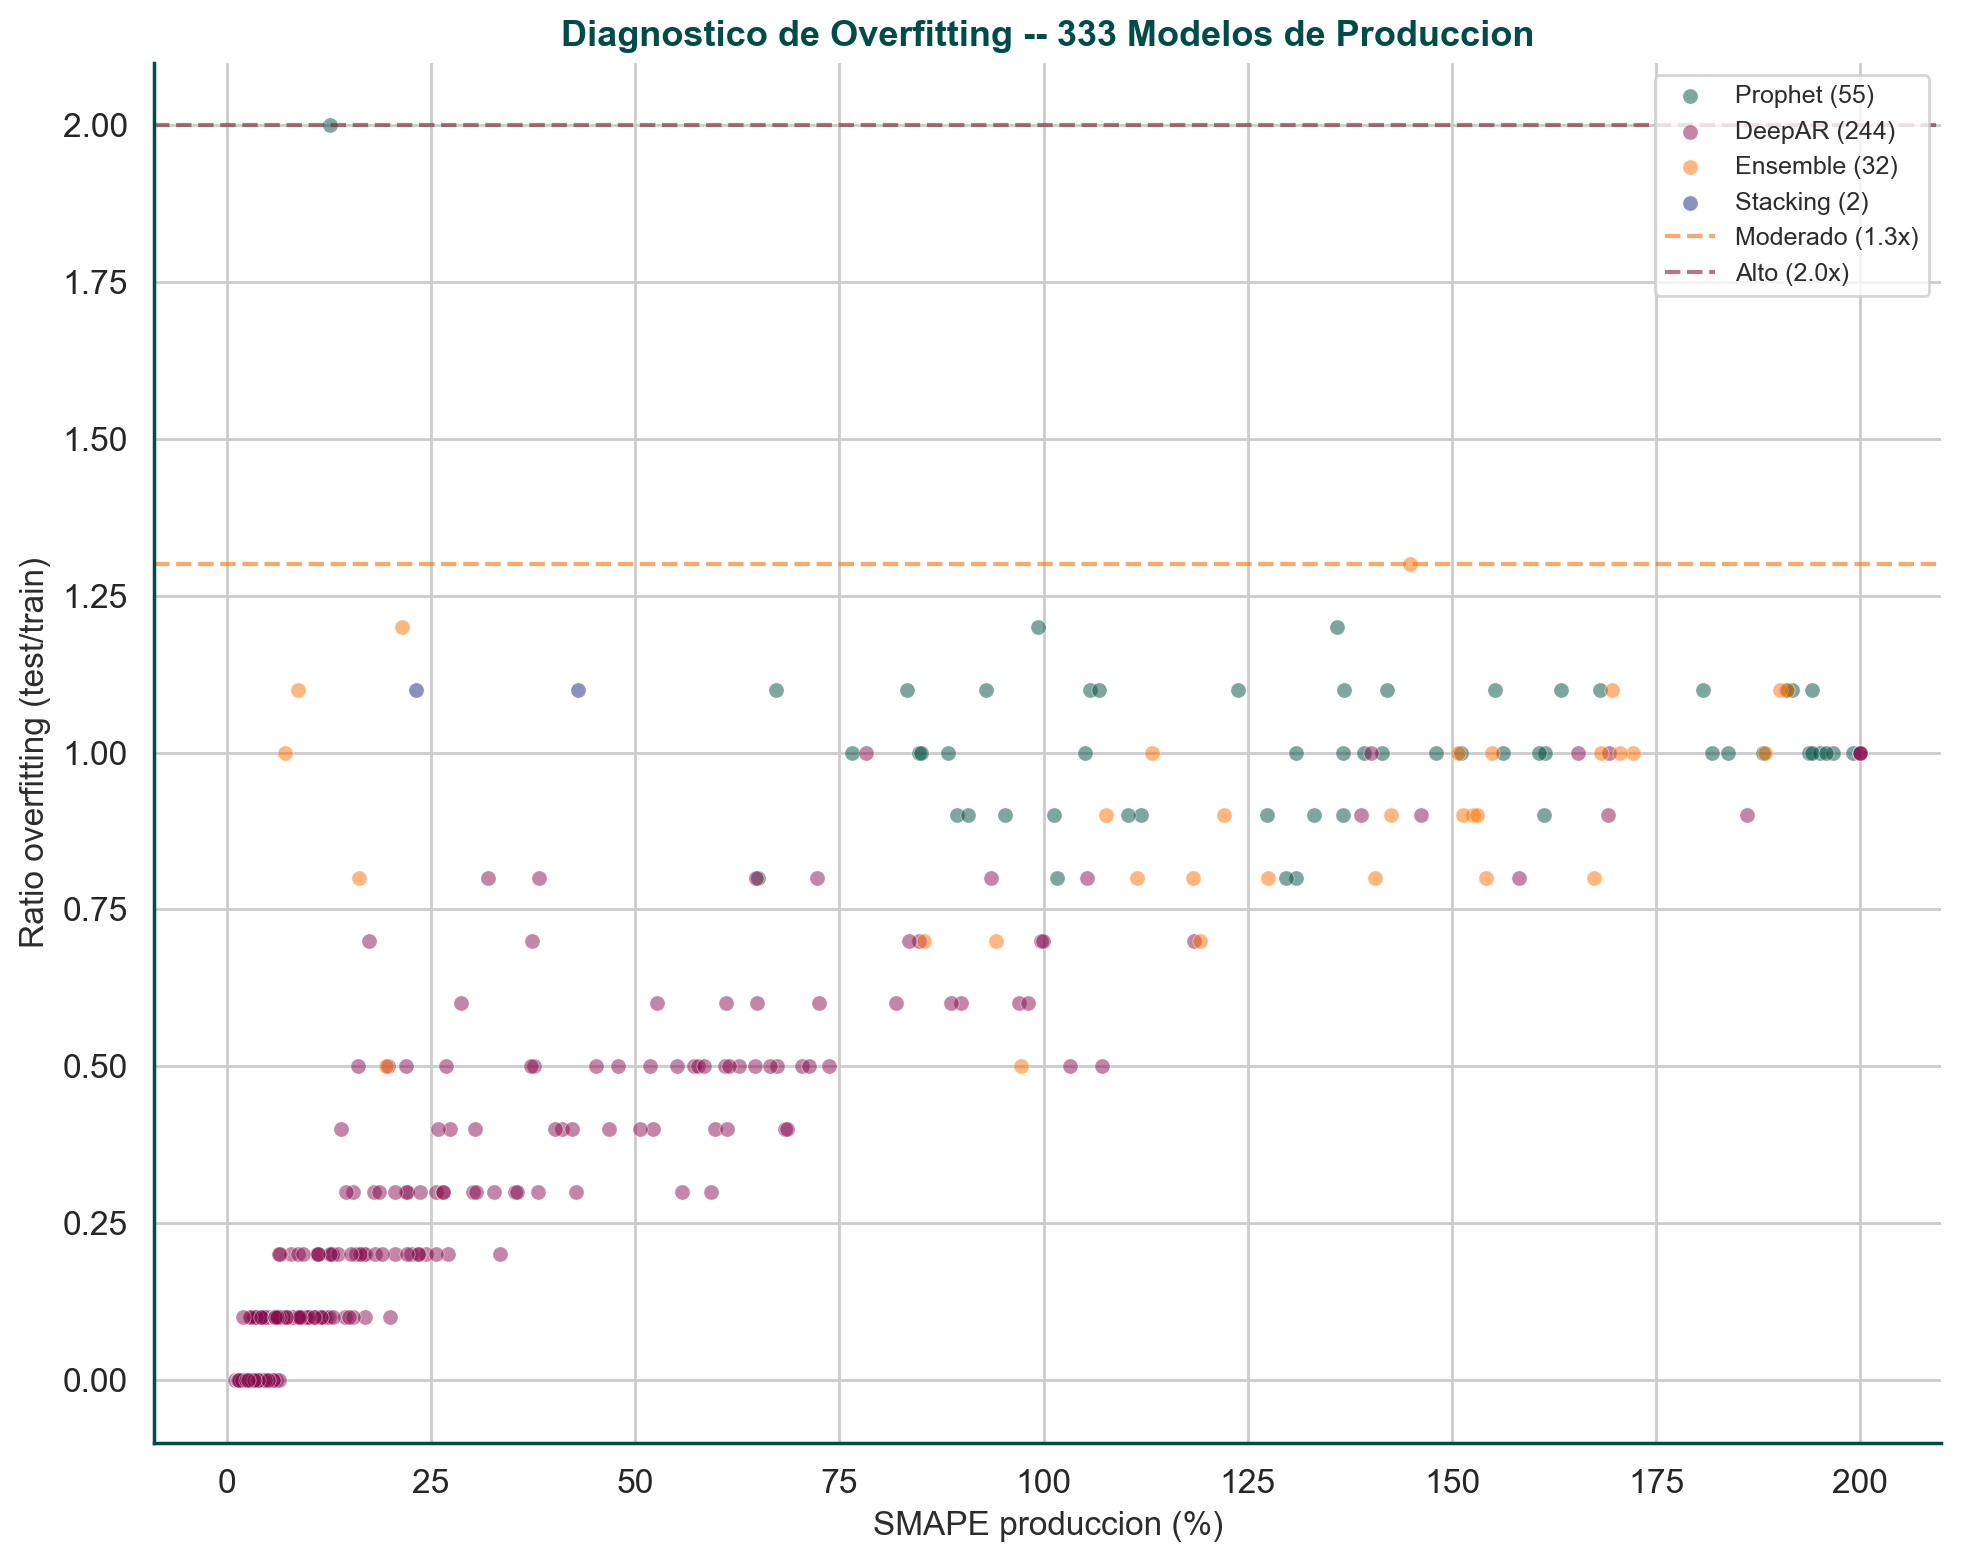
\includegraphics[width=\textwidth]{figuras_avance5/25_scatter_overfitting.png}
        \caption{Scatter de SMAPE test vs.\ train. Los puntos cerca de la diagonal indican ausencia de sobreajuste.}
        \label{fig:scatter_overfit}
    \end{subfigure}
    \hfill
    \begin{subfigure}[t]{0.48\textwidth}
        \centering
        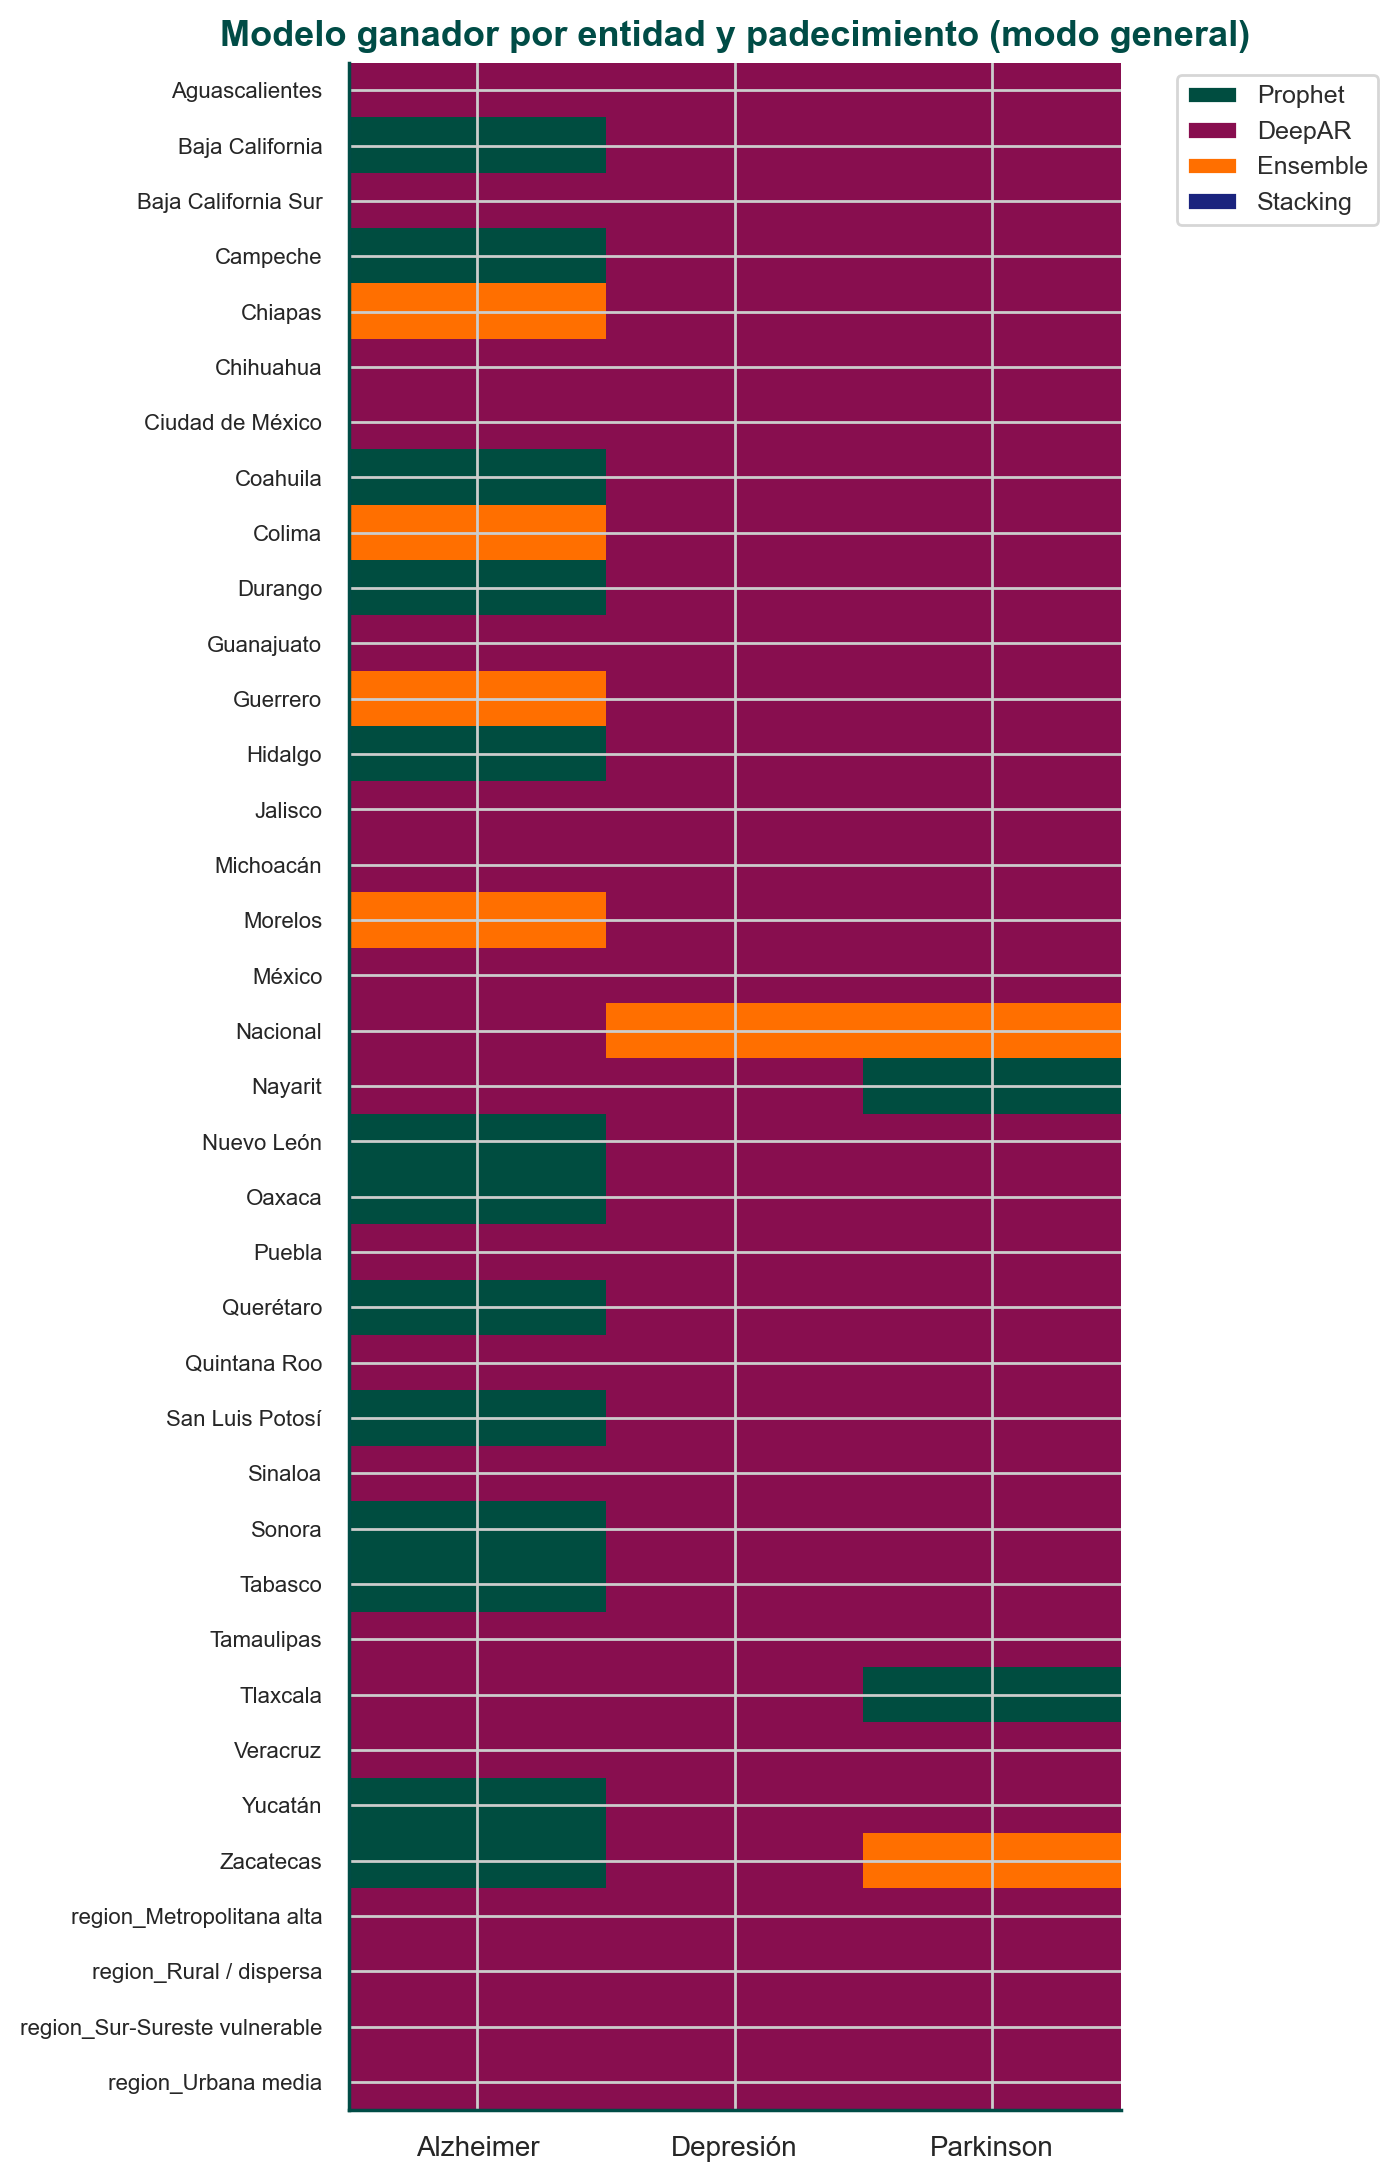
\includegraphics[width=\textwidth]{figuras_avance5/32_matriz_ganador.png}
        \caption{Matriz de frecuencia del modelo ganador por padecimiento y entidad.}
        \label{fig:matriz_ganador}
    \end{subfigure}
    \caption{Diagnosticos de overfitting y seleccion de produccion.}
    \label{fig:overfit_matriz}
\end{figure}

\newpage

\subsection{Graficos Adicionales de Interpretabilidad}

% ---- FIGURAS: Hiperparametros y Seasonality ----
\begin{figure}[H]
    \centering
    \begin{subfigure}[t]{0.48\textwidth}
        \centering
        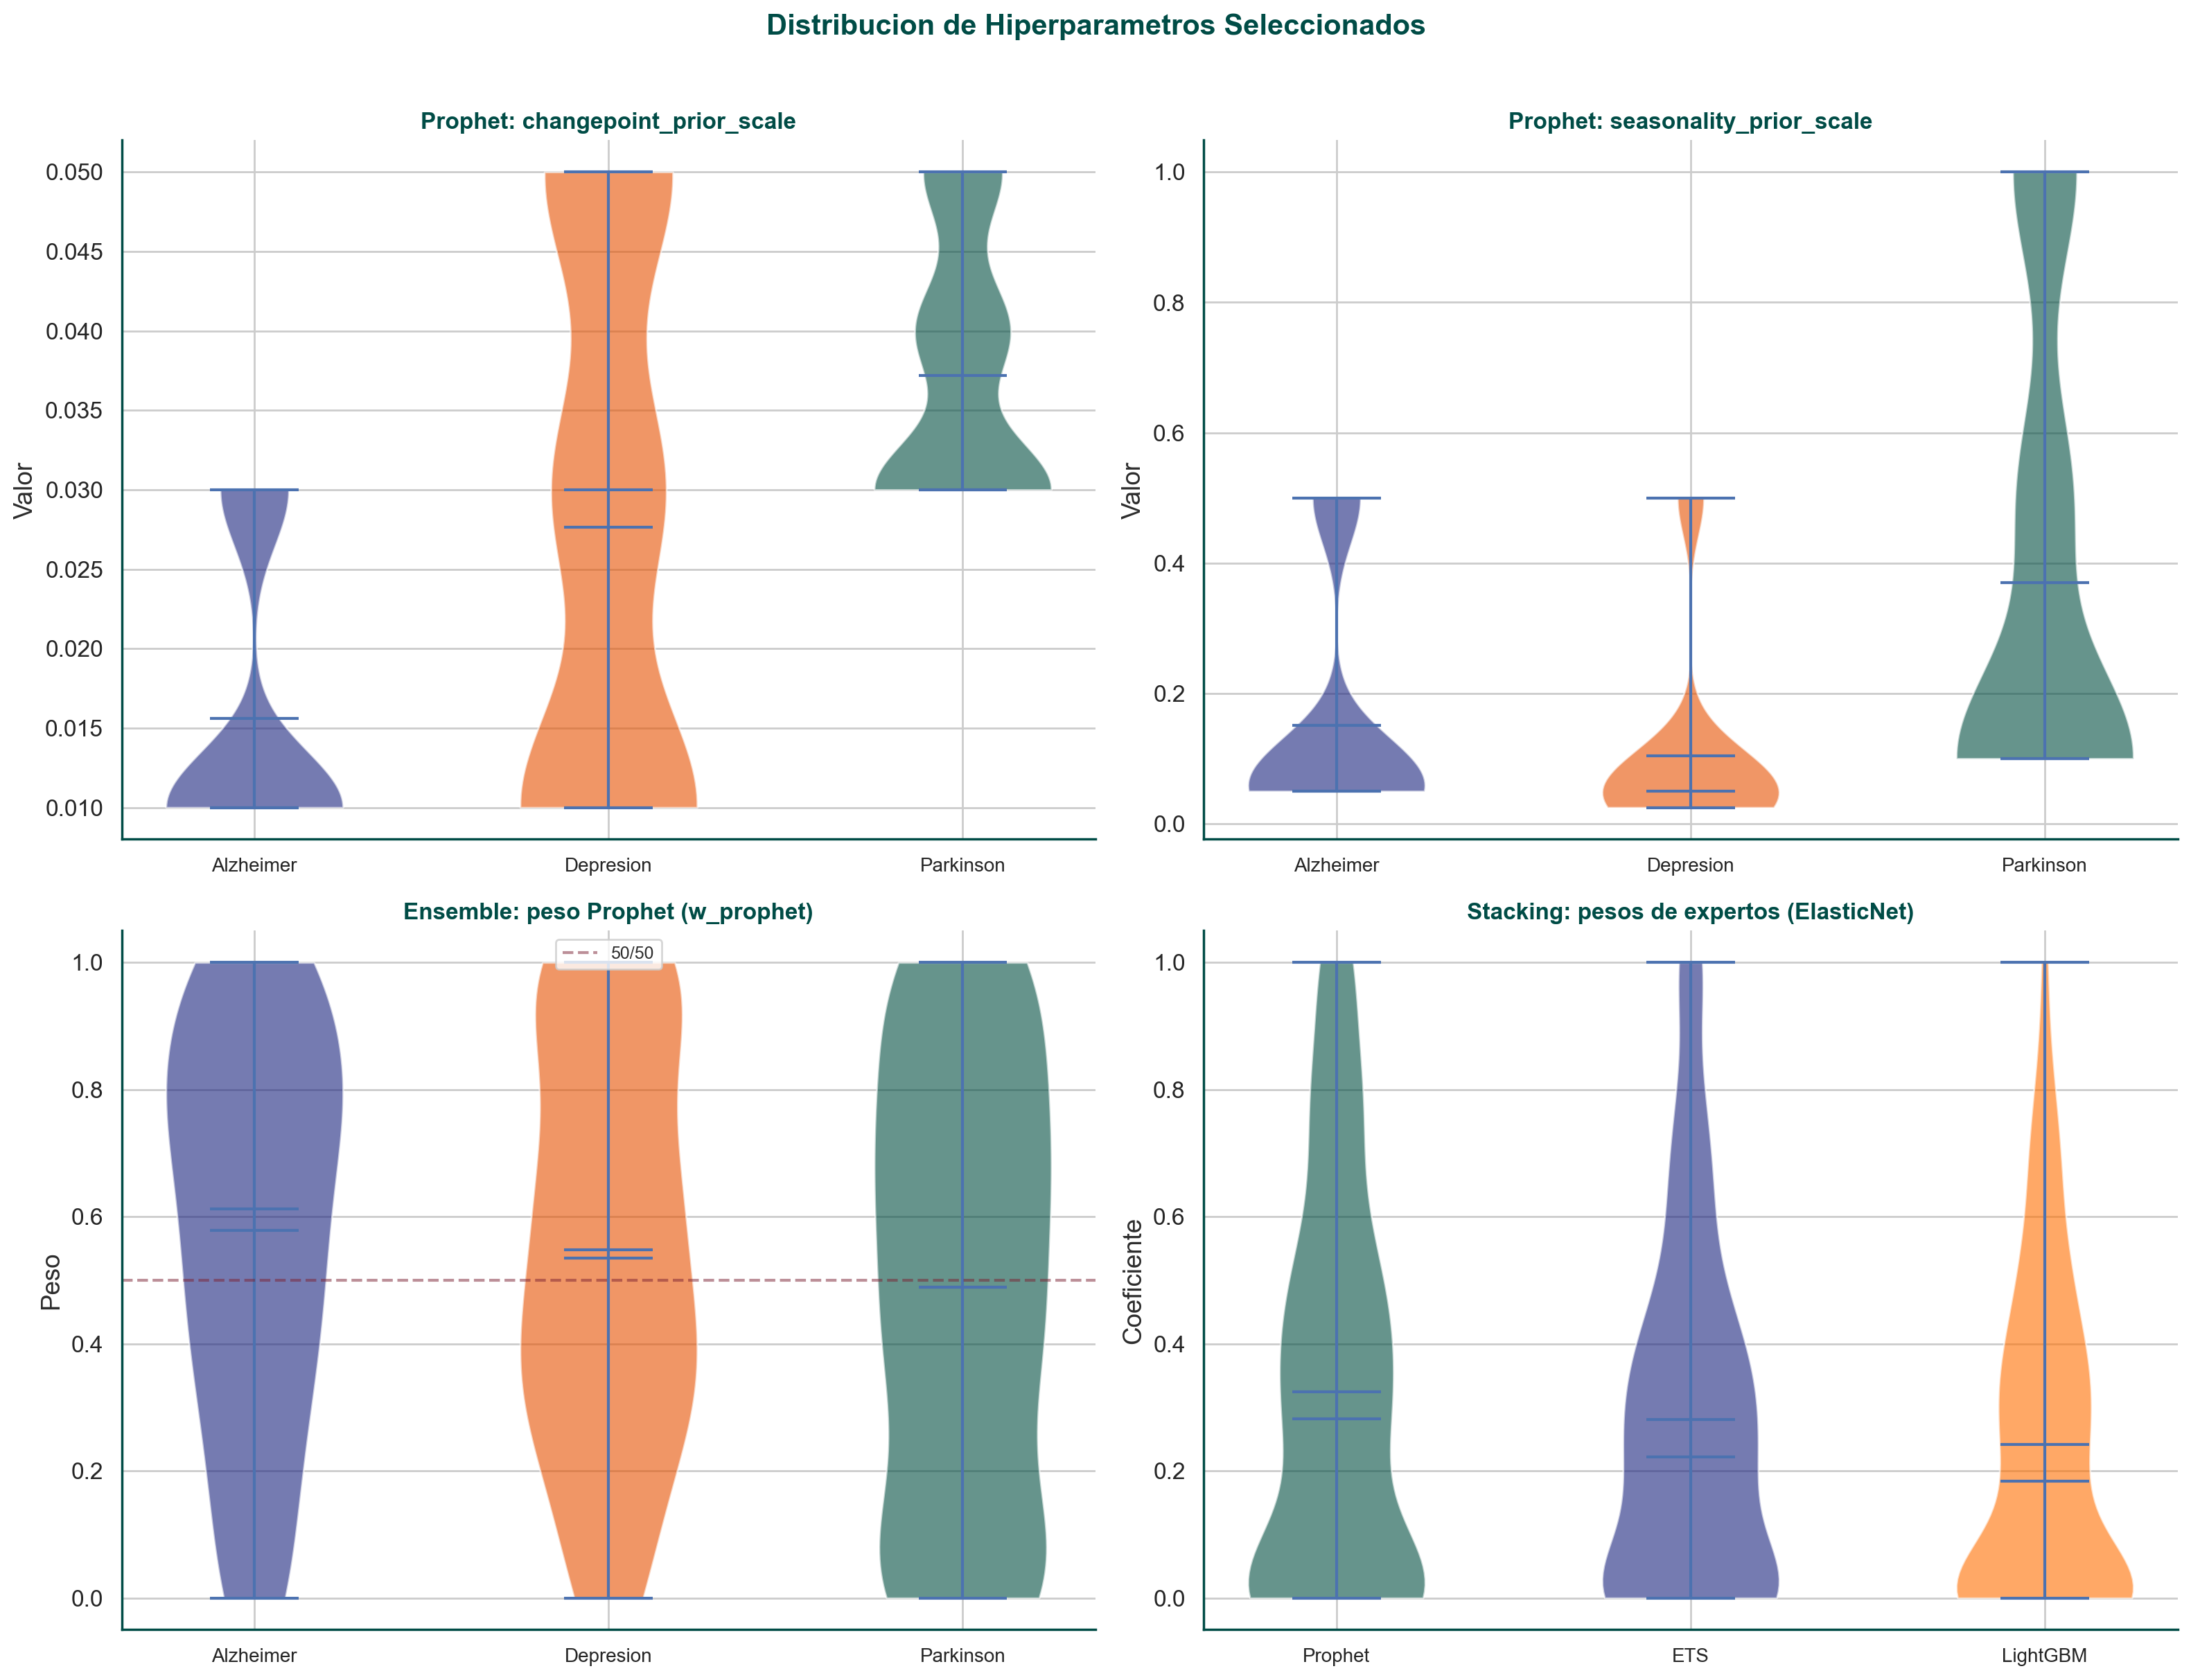
\includegraphics[width=\textwidth]{figuras_avance5/08_violin_hiperparametros.png}
        \caption{Distribucion de hiperparametros optimos de Prophet (violin plot).}
        \label{fig:violin_hp}
    \end{subfigure}
    \hfill
    \begin{subfigure}[t]{0.48\textwidth}
        \centering
        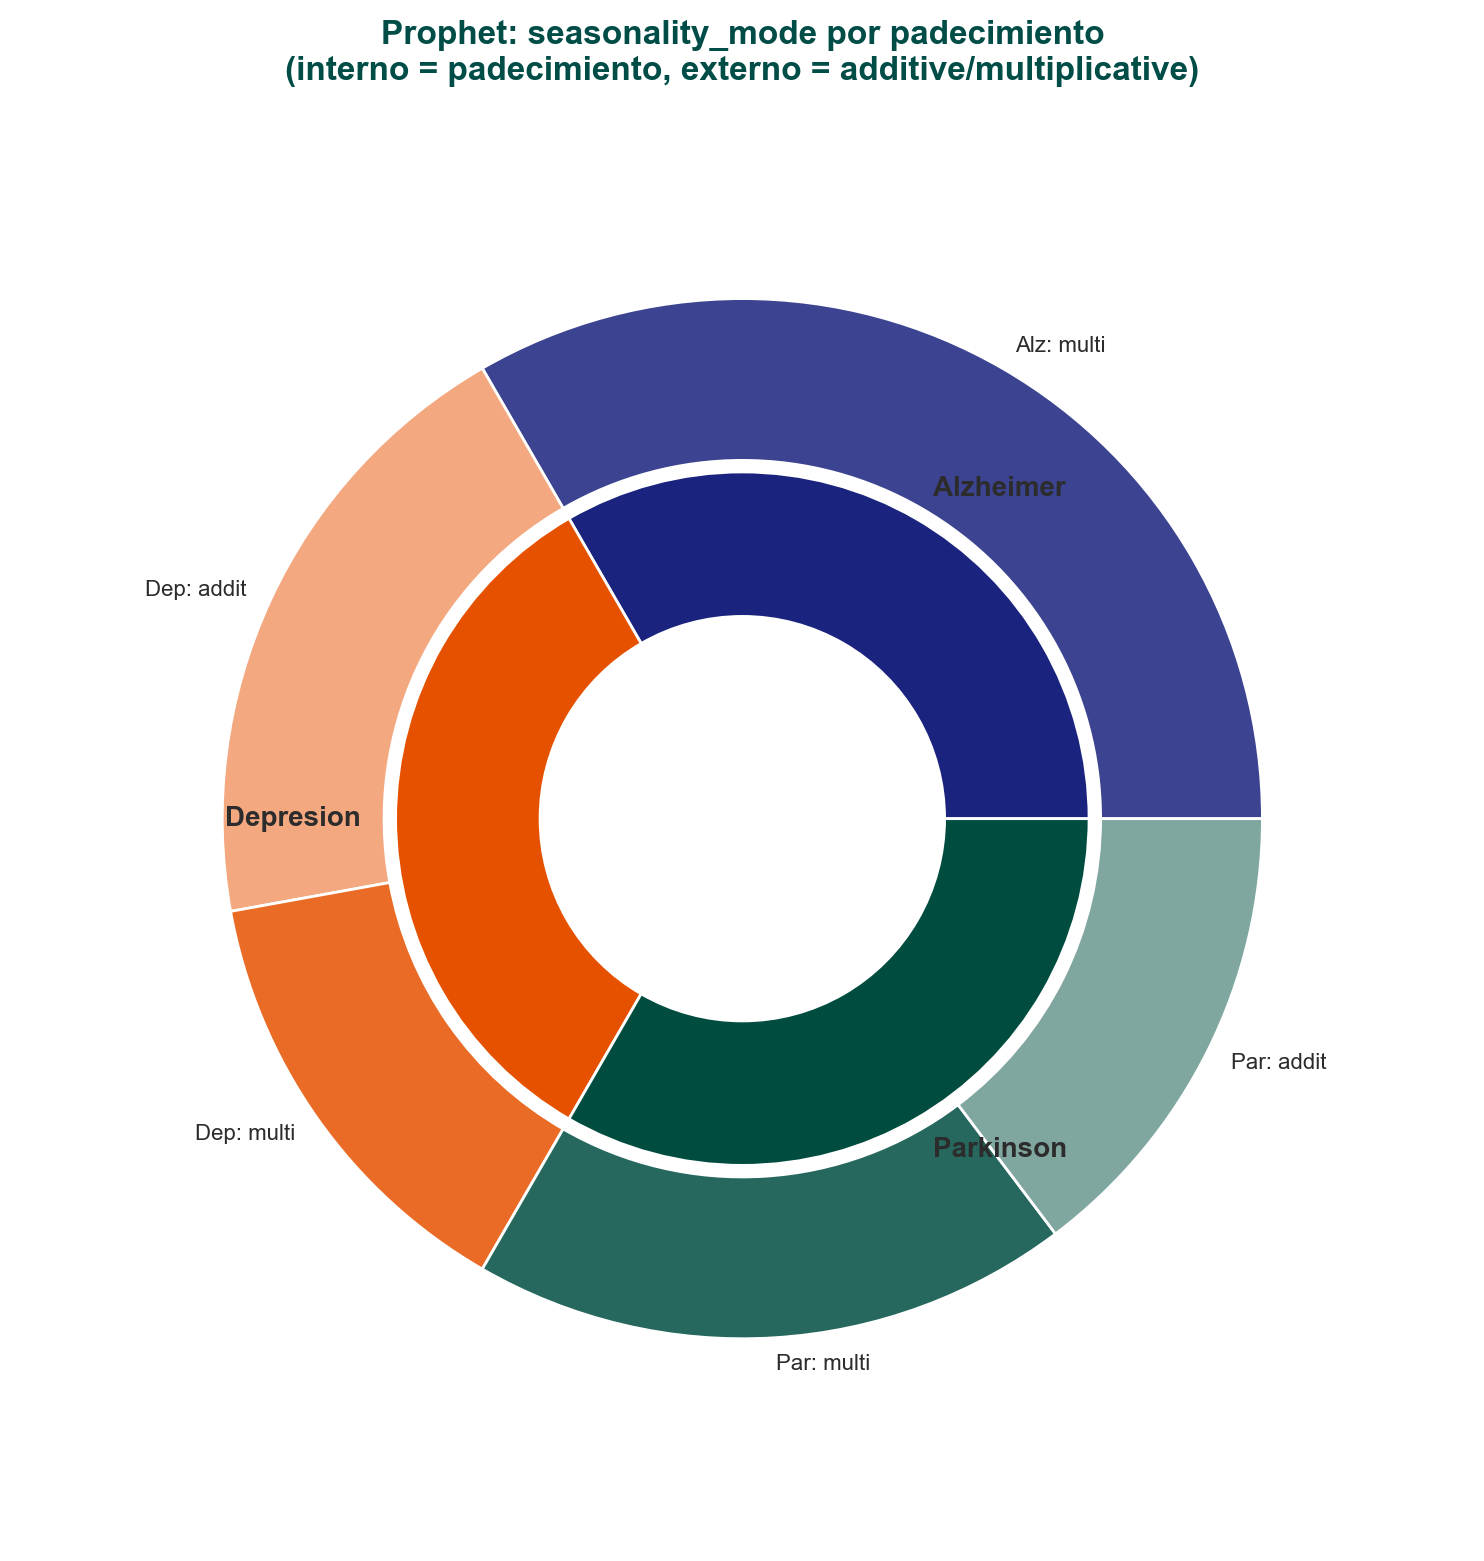
\includegraphics[width=\textwidth]{figuras_avance5/09_donut_seasonality.png}
        \caption{Modo de estacionalidad seleccionado: 65.8\% multiplicativo vs.\ 34.2\% aditivo.}
        \label{fig:donut_season}
    \end{subfigure}
    \caption{Analisis de hiperparametros de Prophet sobre los 333 modelos.}
    \label{fig:hp_season}
\end{figure}

% ---- FIGURAS: Ternario, Stacking coefs, Frontera ----
\begin{figure}[H]
    \centering
    \begin{subfigure}[t]{0.48\textwidth}
        \centering
        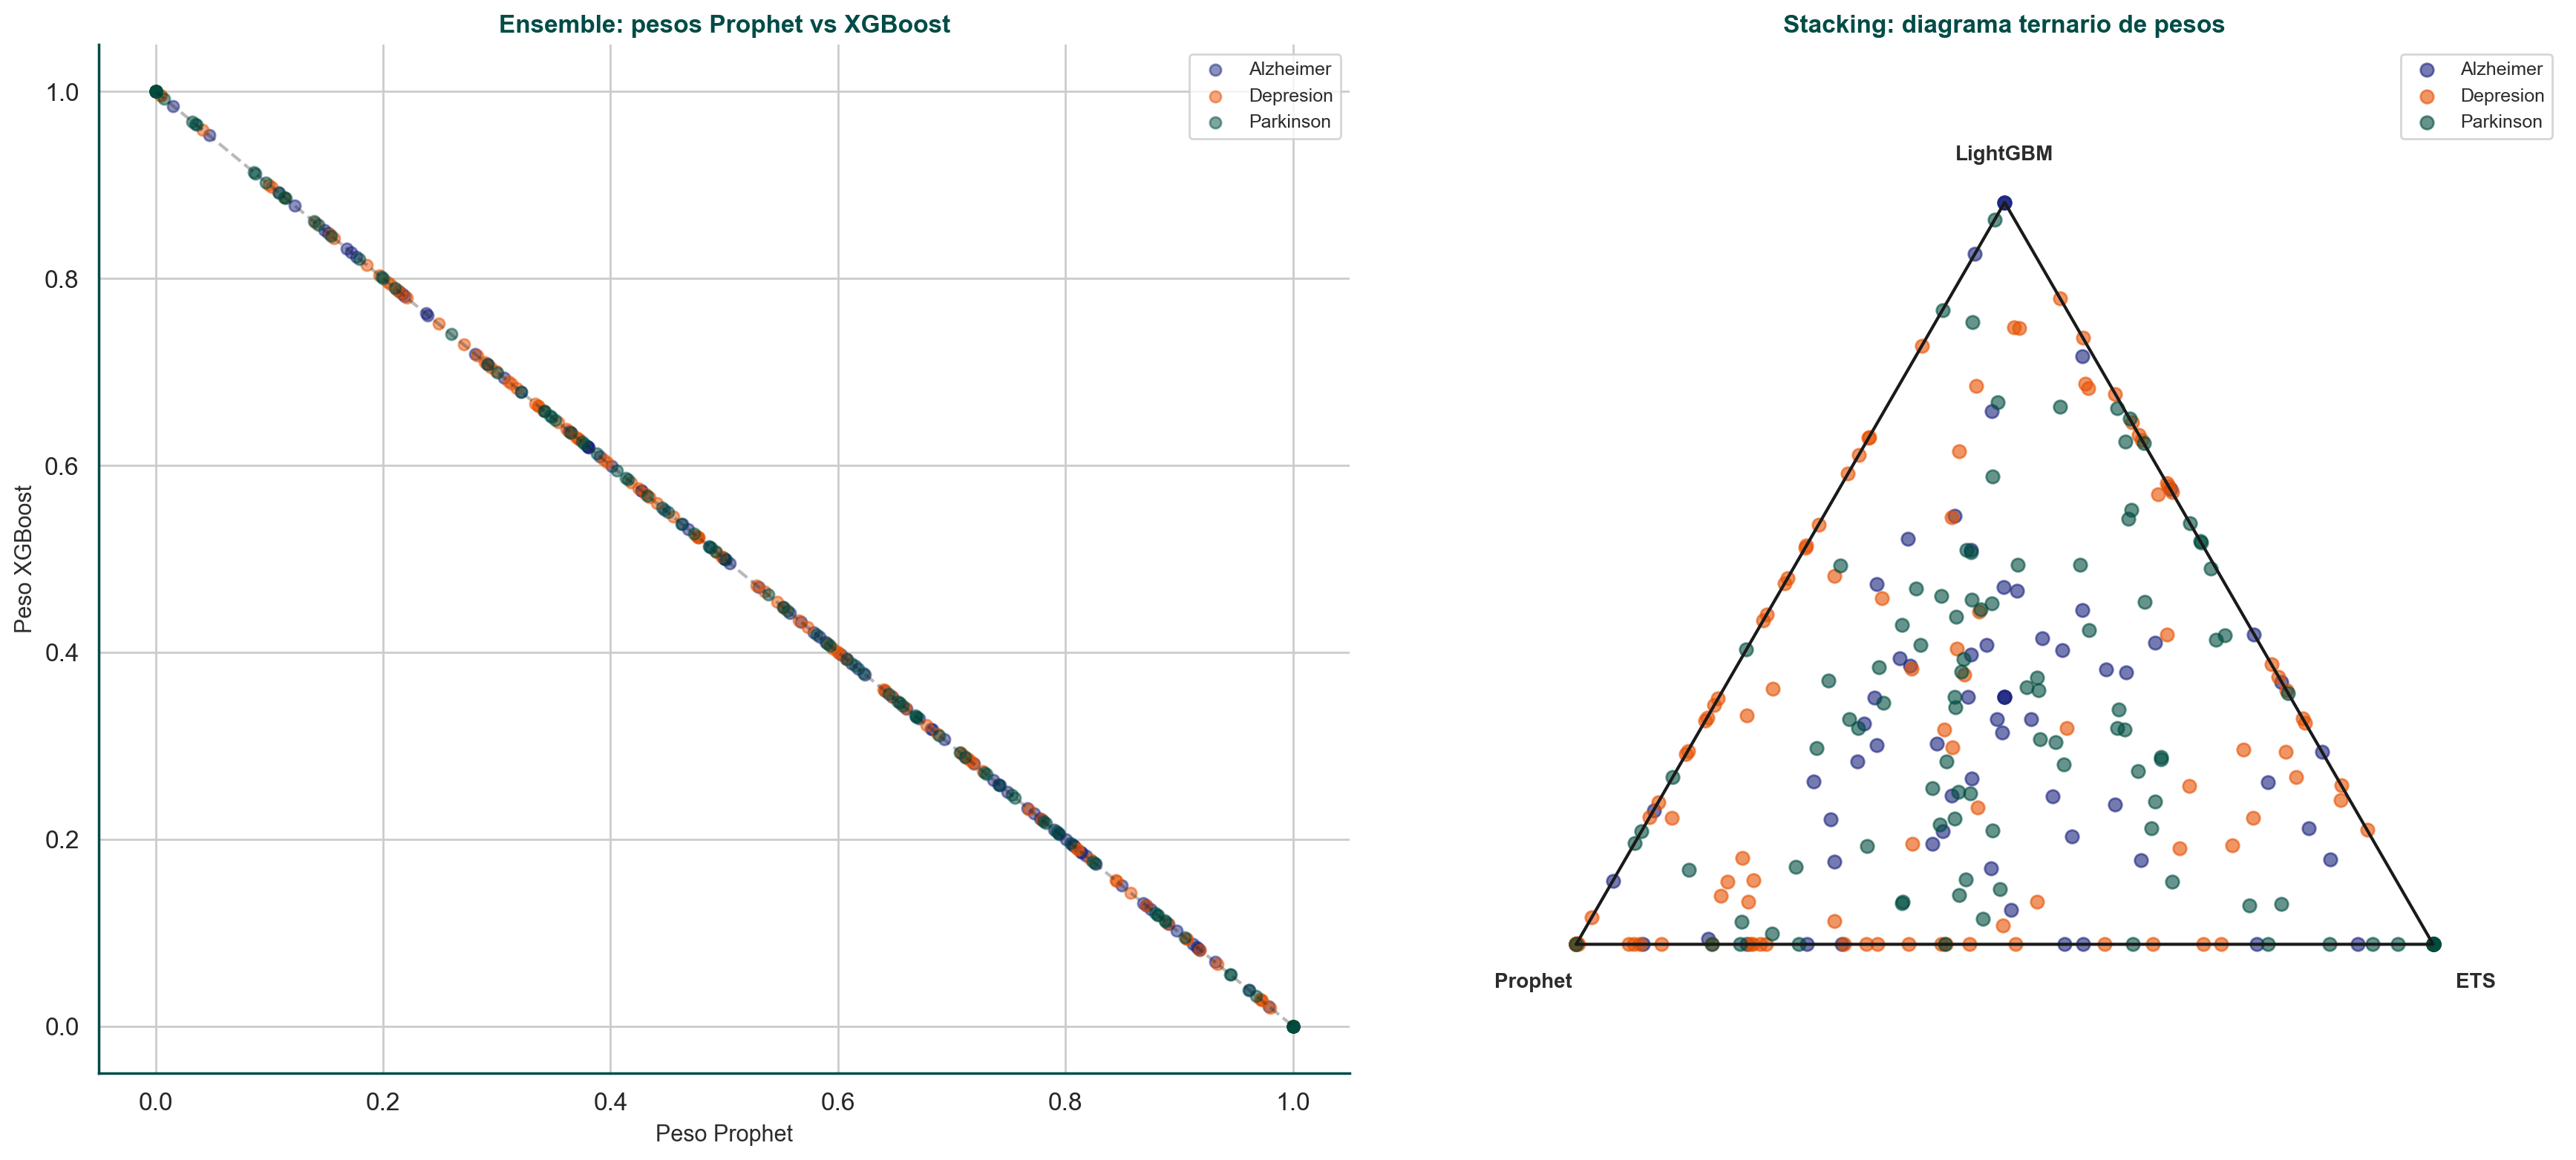
\includegraphics[width=\textwidth]{figuras_avance5/18_ternario_pesos.png}
        \caption{Diagrama ternario de pesos del Stacking (Prophet/ETS/LightGBM).}
        \label{fig:ternario}
    \end{subfigure}
    \hfill
    \begin{subfigure}[t]{0.48\textwidth}
        \centering
        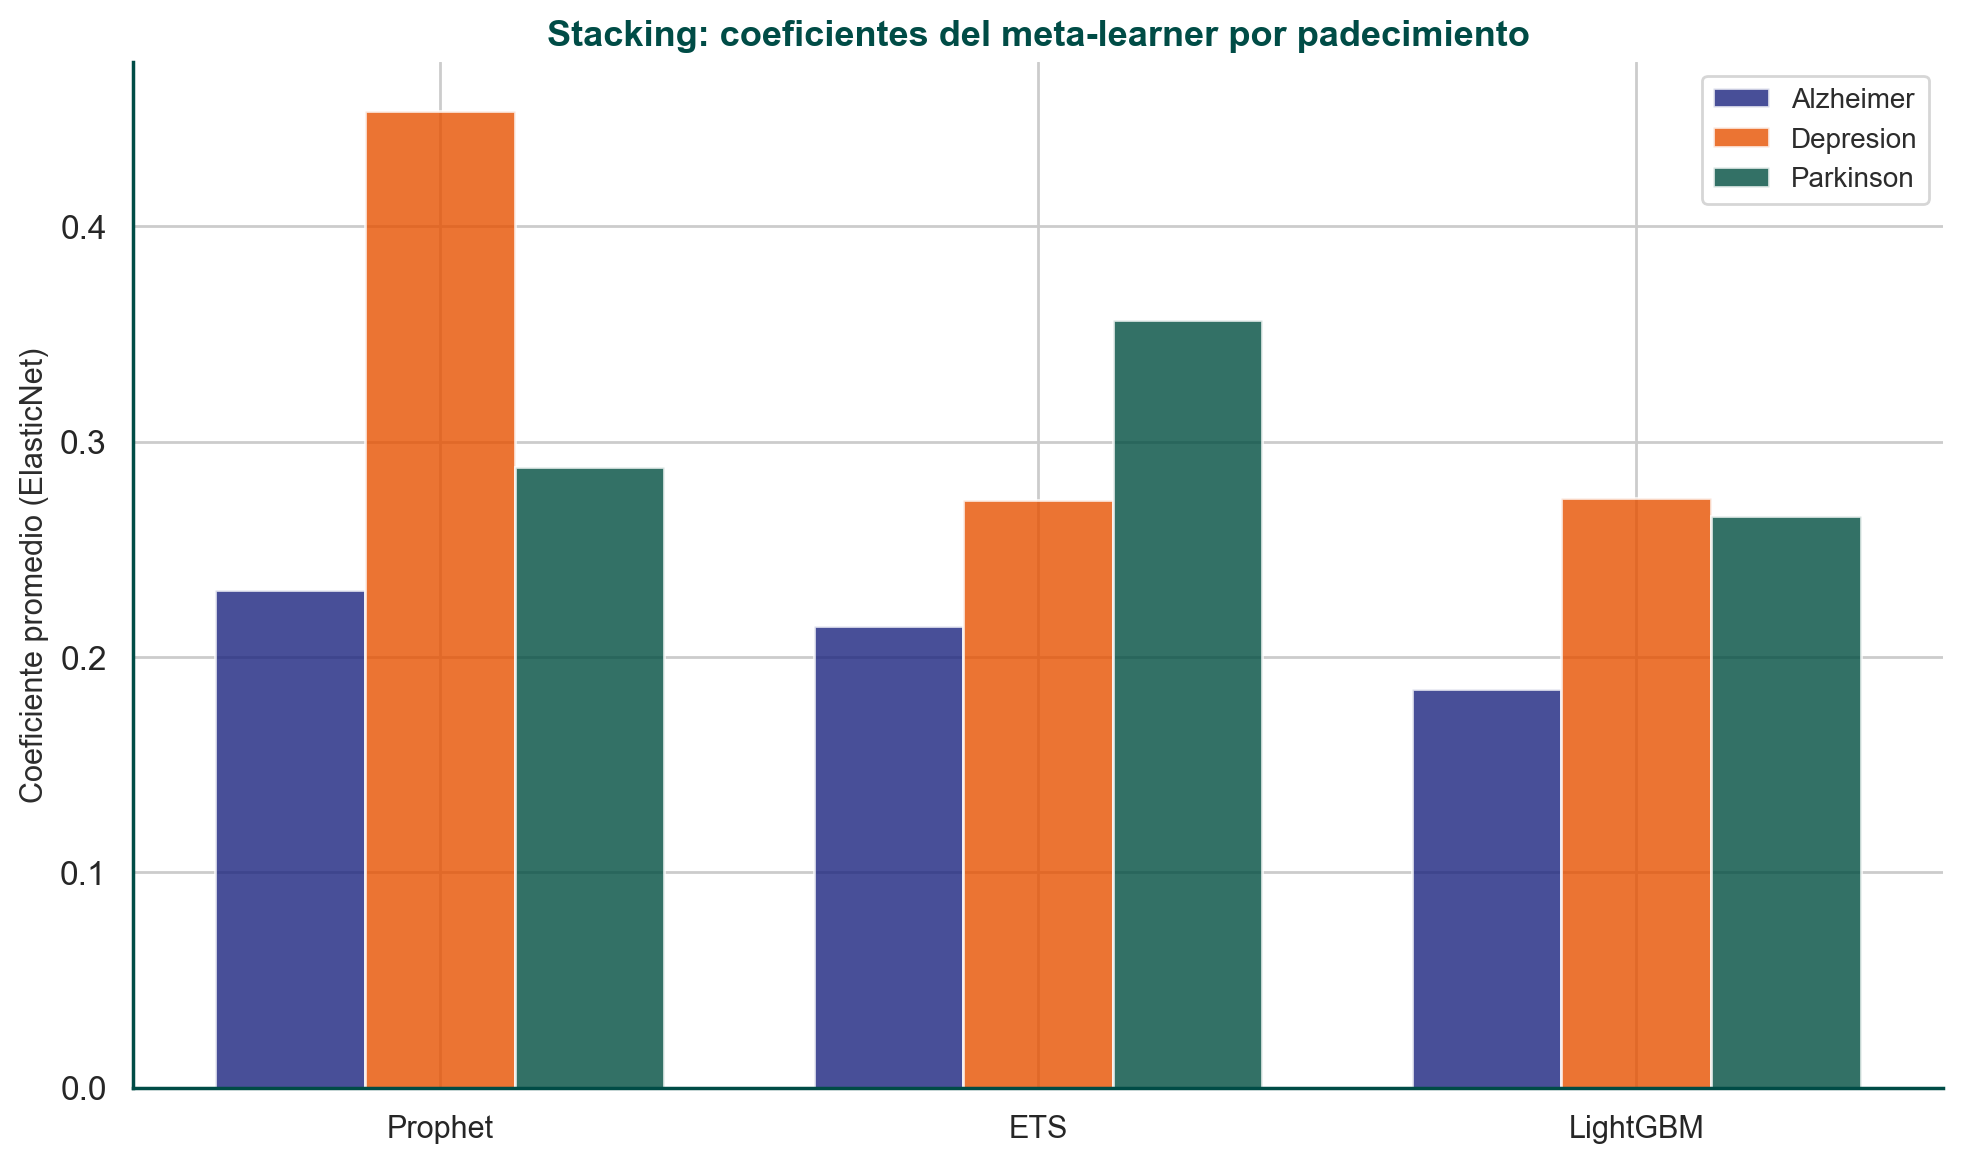
\includegraphics[width=\textwidth]{figuras_avance5/20_stacking_coeficientes.png}
        \caption{Coeficientes del meta-learner ElasticNet por serie.}
        \label{fig:stacking_coefs}
    \end{subfigure}
    \caption{Visualizacion de pesos del modelo Stacking.}
    \label{fig:stacking_viz}
\end{figure}

\begin{figure}[H]
    \centering
    \begin{subfigure}[t]{0.48\textwidth}
        \centering
        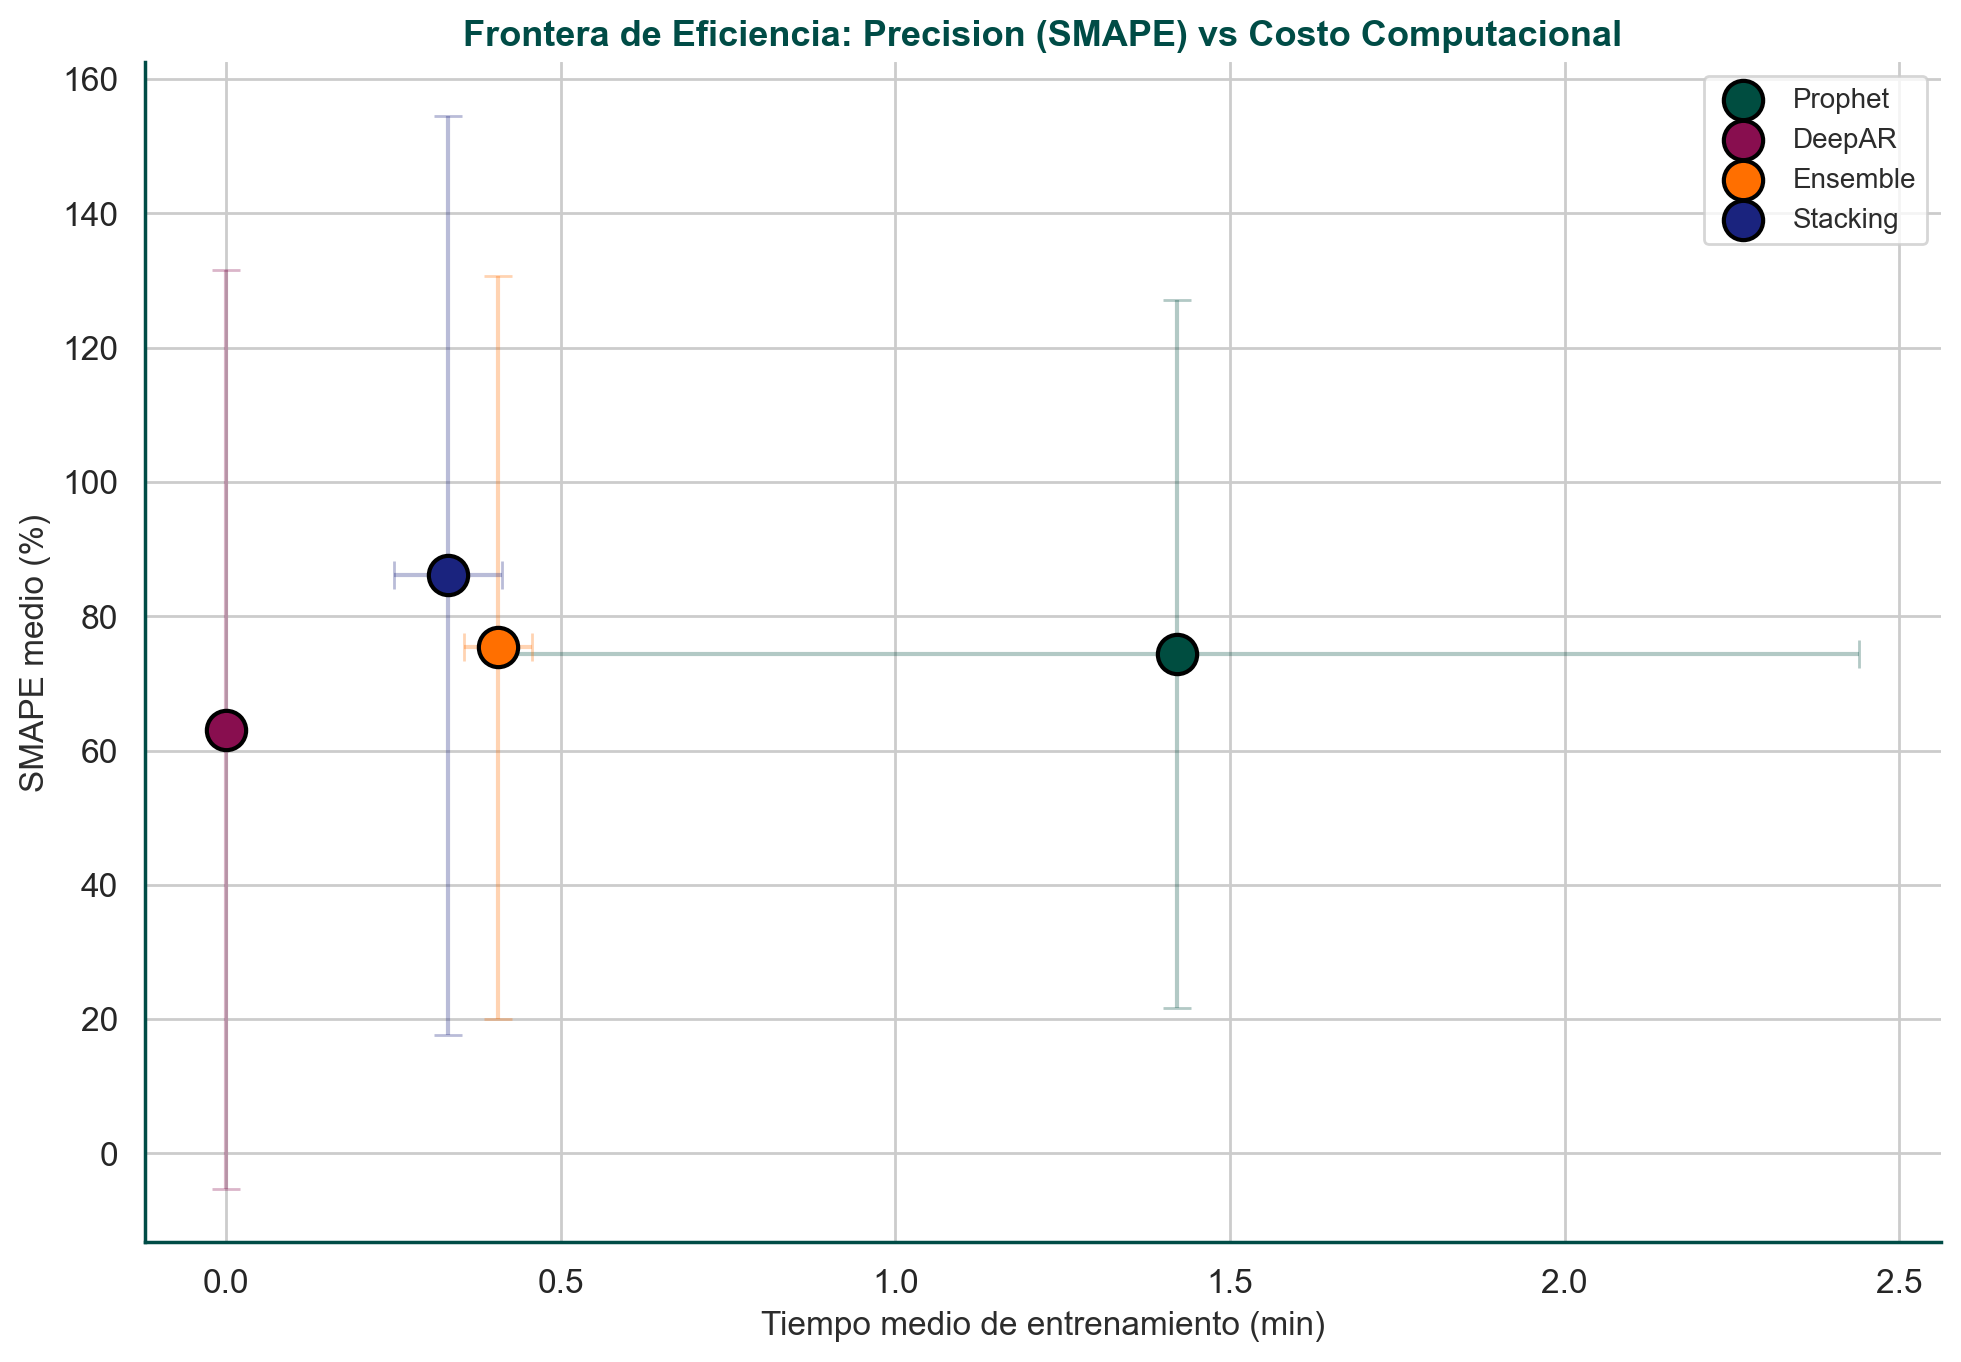
\includegraphics[width=\textwidth]{figuras_avance5/33_frontera_eficiencia.png}
        \caption{Frontera de eficiencia SMAPE vs.\ tiempo de entrenamiento.}
        \label{fig:frontera}
    \end{subfigure}
    \hfill
    \begin{subfigure}[t]{0.48\textwidth}
        \centering
        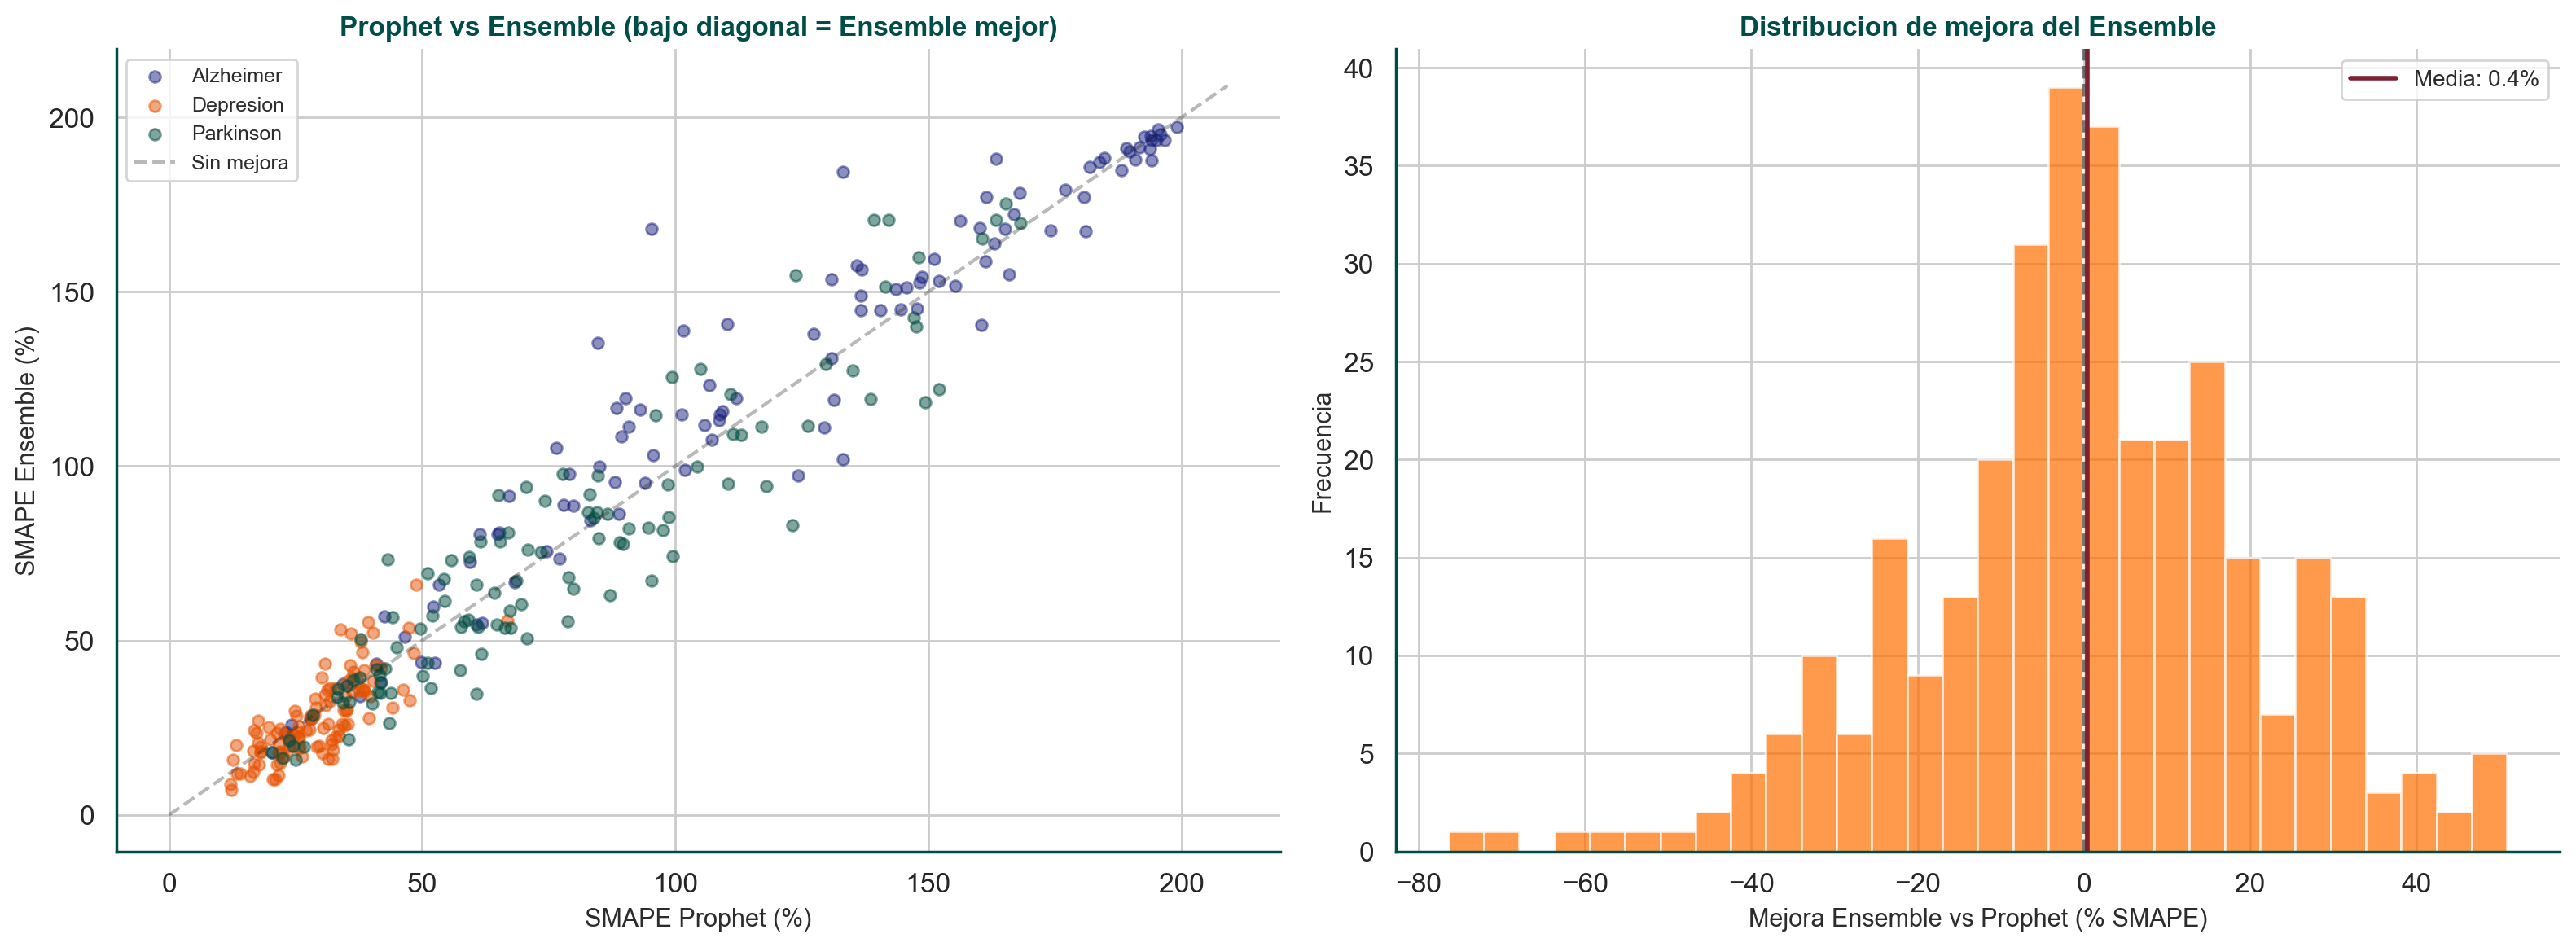
\includegraphics[width=\textwidth]{figuras_avance5/34_mejora_ensemble.png}
        \caption{Mejora porcentual del Ensemble sobre Prophet (baseline).}
        \label{fig:mejora}
    \end{subfigure}
    \caption{Analisis de eficiencia y mejora incremental.}
    \label{fig:eficiencia}
\end{figure}

% ---- FIGURA: Stacked bar produccion ----
\begin{figure}[H]
    \centering
    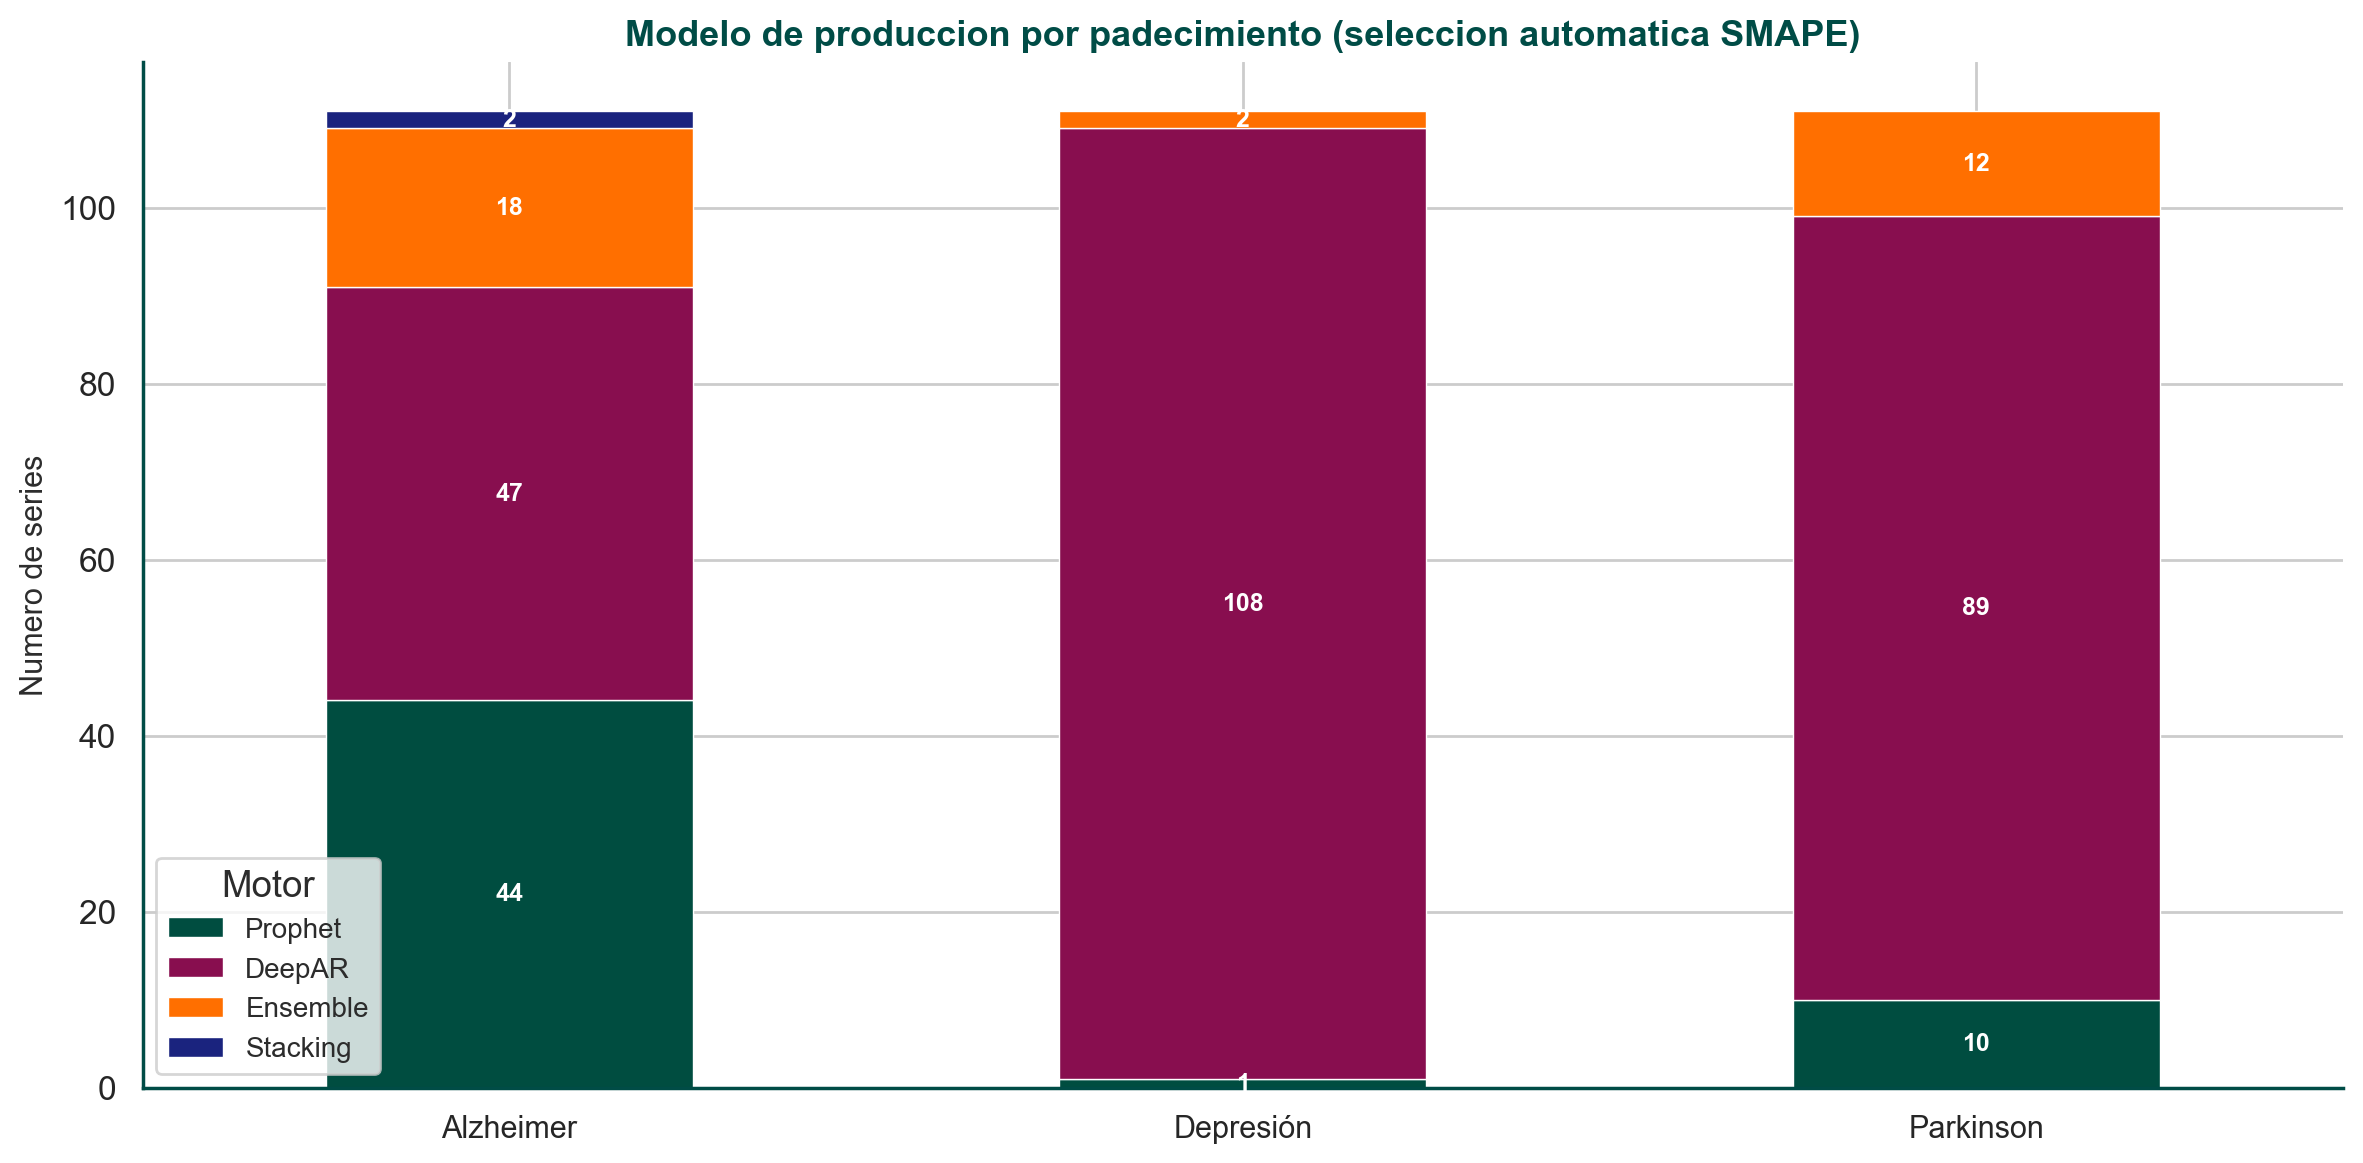
\includegraphics[width=0.80\textwidth]{figuras_avance5/24_stacked_bar_produccion.png}
    \caption{\textbf{Barras apiladas:} distribucion del modelo ganador por padecimiento y sexo. DeepAR domina Depresion y Parkinson; Alzheimer muestra competencia cerrada entre DeepAR y Prophet.}
    \label{fig:stacked_bar}
\end{figure}

\newpage

% =============================================================================
% 8. MLOPS Y ECOSISTEMA TABLEAU
% =============================================================================
\section{MLOps, Tableau y Arquitectura de Produccion}\label{sec:mlops}

\subsection{Pipeline CI/CD y Dashboard}

Se implemento un pipeline CI/CD completo (\texttt{publish\_gsheets.py} via GitHub Actions) para inyectar pronosticos al Dashboard Ejecutivo en Tableau Public.\footnote{Dashboard disponible en \url{https://proyectointegrador.org/epidashboard}}

\begin{criticalbox}[Optimizador frente al Limite de Google Sheets]
Al generar el forecast de los 1,332 modelos, el dataset superaba los \textbf{120 millones de celdas}, chocando contra el limite estricto de la API de Google Sheets (10 millones).

\textbf{Solucion MLOps:} Se construyo un algoritmo de compresion que elimina jerarquias redundantes, reduce el \textit{payload} al 50\%, e inyecta los datos en bloques (\textit{chunks}) cada hora sin intervencion humana. Se han logrado \textbf{163 ejecuciones exitosas consecutivas}.
\end{criticalbox}

\textbf{Rediseno UI:} Atendiendo la recomendacion clinica, el Dashboard se re-estructuro. Los filtros ya no mezclan estados con regiones, y la UI guia al usuario primero por la \textit{Exploracion Historica} antes de mostrar la prediccion de \textbf{casos absolutos} para la logistica hospitalaria.

% ---- FIGURA: KPI Dashboard ----
\begin{figure}[H]
    \centering
    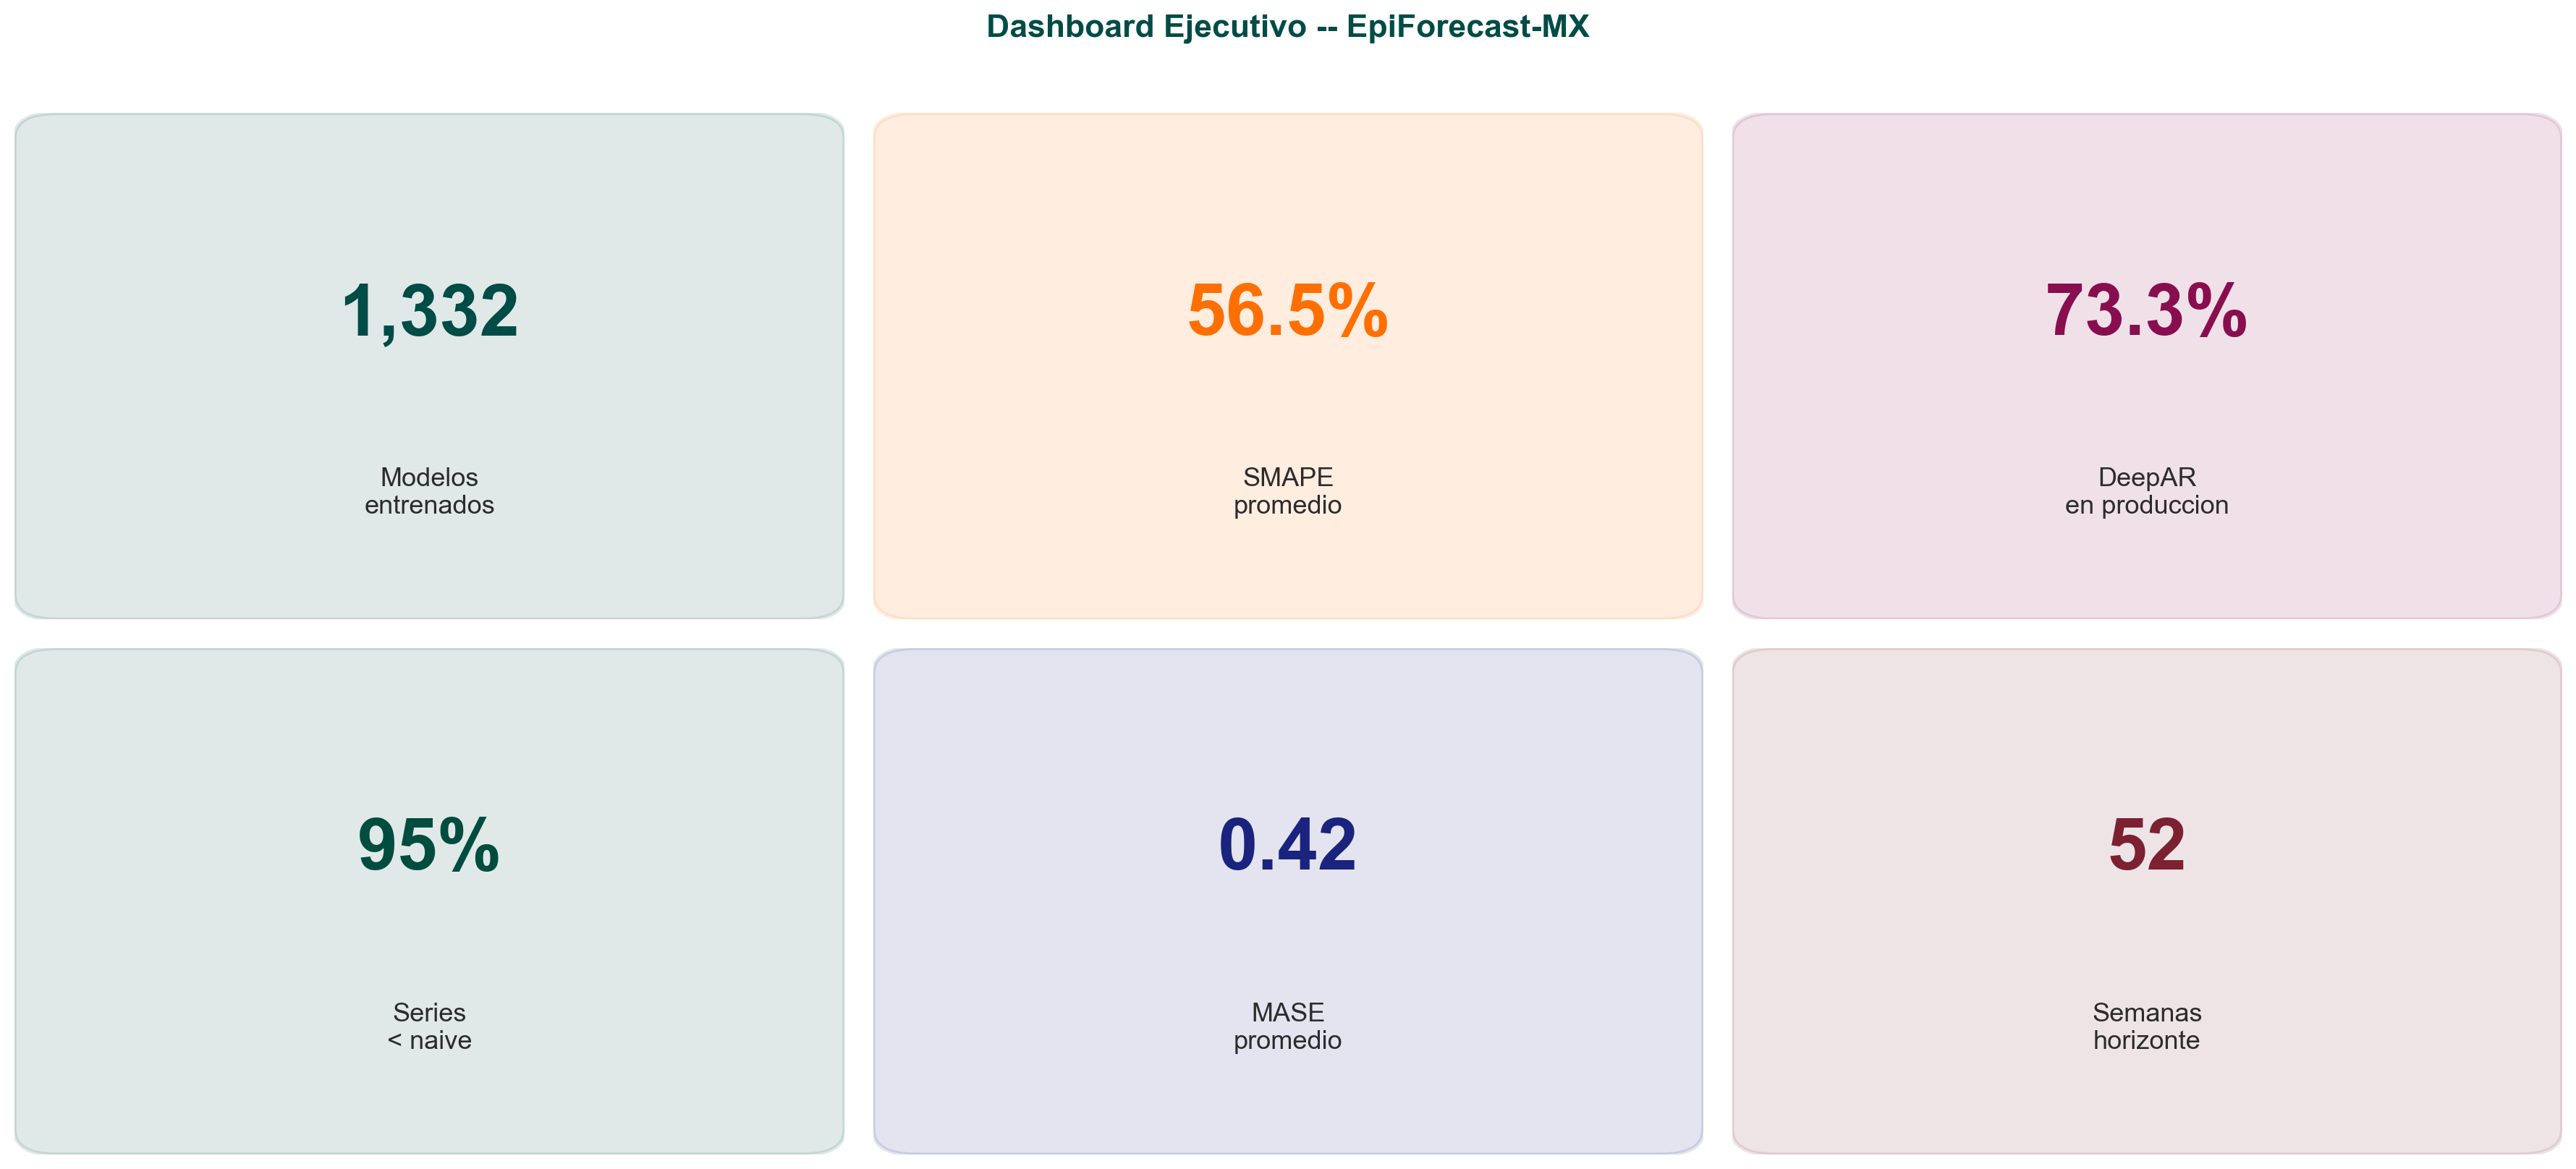
\includegraphics[width=0.9\textwidth]{figuras_avance5/31_kpi_dashboard.png}
    \caption{Panel superior de KPIs ejecutivos de la plataforma EpiForecast-MX en Tableau.}
    \label{fig:kpis}
\end{figure}

\subsection{Infraestructura de Computo}

\begin{table}[H]
\centering
\caption{Tiempos de entrenamiento por motor (333 modelos)}
\label{tab:tiempos}
\small
\begin{tabular}{llrr}
\toprule
\textbf{Motor} & \textbf{Hardware} & \textbf{Tiempo total} & \textbf{Promedio/modelo} \\
\midrule
Prophet   & CPU (Apple M2, joblib $-2$) & 7.9 horas  & 85.2 seg \\
DeepAR    & GPU (AWS SageMaker T4)     & 1.5 horas  & N/A (batch) \\
DeepAR    & CPU/MPS (Apple M2 local)   & 4.0 horas  & N/A (batch) \\
Ensemble  & CPU (Apple M2)             & 2.3 horas  & 24.4 seg \\
Stacking  & CPU (Apple M2)             & 1.8 horas  & 19.9 seg \\
\midrule
\textbf{Total (4 motores)} & & \textbf{$\sim$13.5 horas} & \\
\bottomrule
\end{tabular}
\end{table}

\subsection{Artefactos y Versionamiento}

El sistema genera y versiona via DVC (Data Version Control) conectado a Amazon S3:
\begin{itemize}[noitemsep]
    \item \textbf{1,332 modelos} serializados (\texttt{.pkl}) + \textbf{1,353 CSVs} de forecast.
    \item \textbf{764 pruebas unitarias} (Pytest) con cobertura $>70\%$.
    \item \textbf{333 graficos individuales} del modelo ganador (\texttt{PROD\_MODELS/}).
    \item Pre-commit hooks: Ruff (lint + format), Mypy (tipado estricto), trailing whitespace.
    \item MLflow local para tracking de experimentos (metricas, parametros, tiempos).
\end{itemize}

\newpage

% =============================================================================
% 9. CONCLUSIONES
% =============================================================================
\section{Conclusiones}\label{sec:conclusiones}

\begin{enumerate}
    \item \textbf{Mejora demostrable (Objetivo 3.5):} La introduccion de \textit{Ensemble Learning} mitigo las debilidades del modelo base. El Ensemble con XGBoost inyecto reaccion a la volatilidad post-COVID, y DeepAR resolvio el ruido en series con ceros mediante \textit{transfer learning}. A nivel global, DeepAR reduce el SMAPE un \textbf{15\%} respecto a Prophet (63.13\% vs.\ 74.42\%).

    \item \textbf{Calidad en datos no vistos (Objetivo 3.6):} La reingenieria etica del \textit{backtest} de ventana expansiva garantizo metricas honestas. La eliminacion de dos fuentes de \textit{data leakage} (en preprocesamiento y en features del Ensemble) y la implementacion de 764 tests automatizados aseguran la integridad del pipeline.

    \item \textbf{El paradigma Multi-motor:} No existe un algoritmo universal. DeepAR domina el 73.3\% de las series (nivel micro), mientras que Ensemble y Prophet prevalecen en agregados macro y series de bajo volumen, respectivamente. El enrutador dinamico asigna el mejor motor para cada una de las 333 combinaciones clinicas.

    \item \textbf{Robustez clinica:} El 98.5\% de los modelos de produccion presentan overfitting controlado ($<1.3\times$) y el 99.1\% esta libre de sospecha de leakage. Las 8 series con incidencia insuficiente se reasignan automaticamente a su modelo regional.

    \item \textbf{Pronosticos accionables:} El sistema proyecta \textbf{451,571 casos de Depresion}, \textbf{23,775 de Parkinson} y \textbf{7,212 de Alzheimer} para las proximas 52 semanas, informacion que permite al IMSS planificar camas, insumos y personal con anticipacion.
\end{enumerate}

\newpage

% =============================================================================
% 10. REFLEXIONES PERSONALES DEL EQUIPO
% =============================================================================
\section{Reflexiones Personales del Equipo}\label{sec:reflexiones}

\begin{minipage}[t]{0.18\textwidth}
    \vspace{0pt}
    \includegraphics[width=\linewidth, clip, trim=0 0 0 0]{JARS20206.jpg}
\end{minipage}%
\hfill
\begin{minipage}[t]{0.78\textwidth}
    \vspace{0pt}
    \textbf{Javier Augusto Rebull Saucedo} \\
    \textit{\small Sr.\ Associate Development Application -- Santander Bank US}

    \smallskip
    El paso hacia Ensemble Learning redefinio el concepto de escalabilidad en nuestro sistema. Descubrir que DeepAR domina a nivel estatal pero pierde contra XGBoost a nivel Nacional me enseno el valor del diseno MLOps. Construir un enrutador inteligente que selecciona dinamicamente entre 4 motores basandose en el SMAPE de prueba fue el reto de ingenieria mas satisfactorio. La deteccion de \textit{data leakage} en el feature builder nos obligo a repensar cada supuesto: una leccion que aplico ahora en mi trabajo diario en banca.
\end{minipage}

\vspace{0.8cm}

\begin{minipage}[t]{0.18\textwidth}
    \vspace{0pt}
    
\includegraphics[width=\linewidth, clip, trim=0 0 0 0]{JARCOS2026.png}
\end{minipage}%
\hfill
\begin{minipage}[t]{0.78\textwidth}
    \vspace{0pt}
    \textbf{Juan Carlos Perez Nava} \\
    \textit{\small Head of Area -- Instituto Mexicano del Seguro Social (IMSS)}

    \smallskip
    Validar que el modelo traduzca matematicas (tasas por 100k) en \textbf{casos absolutos} en el Dashboard cerro el circulo con el negocio. El IMSS planea con pacientes reales, no con coeficientes. Ver como XGBoost y DeepAR corrigieron la suavidad excesiva de Prophet me demostro que confiar en la diversidad algoritmica y superar barreras tecnicas (como el limite de Google Sheets) convierte un ejercicio academico en una herramienta de salud publica. El fallback regional para series de ceros fue un diseno que nacio de la necesidad clinica real.
\end{minipage}

\vspace{0.8cm}

\begin{minipage}[t]{0.18\textwidth}
    \vspace{0pt}
    
\includegraphics[width=\linewidth, clip, trim=0 0 0 0]{LUIS2026.jpg}
\end{minipage}%
\hfill
\begin{minipage}[t]{0.78\textwidth}
    \vspace{0pt}
    \textbf{Luis Gerardo Sanchez Salazar} \\
    \textit{\small Sr.\ Controls Engineer -- Tesla}

    \smallskip
    La topologia del Stacking resono con mi formacion en ingenieria de controles: un \textit{meta-learner} actuando como un controlador PID que ajusta pesos dinamicamente segun la epoca del ano (gracias a las variables seno/coseno). Detectar y corregir el \textit{data leakage} historico en GluonTS fue un triunfo etico. Programar la ventana expansiva real nos costo horas de GPU, pero doto al sistema de residuales honestos y bandas de confianza autenticas. La batalla contra la convergencia del ElasticNet en series de ceros nos enseno que la robustez no es opcional: es la diferencia entre un prototipo y un sistema de produccion.
\end{minipage}

\newpage

% =============================================================================
% REFERENCIAS
% =============================================================================
\section*{Referencias}
\addcontentsline{toc}{section}{Referencias}

\begin{enumerate}[label={[\arabic*]}, leftmargin=*, noitemsep]
    \itemSingh, A. (2023). Comprehensive Guide to Ensemble Learning. \textit{Analytics Vidhya}.

    \itemVanderPlas, J. (2022). Thinking About Model Validation. En \textit{Python Data Science Handbook} (2nd ed., pp.~410--427). O'Reilly Media.

    \itemSalinas, D., Flunkert, V., Gasthaus, J. \& Januschowski, T. (2020). DeepAR: Probabilistic forecasting with autoregressive recurrent networks. \textit{International Journal of Forecasting}, 36(3), 1181--1191.

    \itemTaylor, S.\,J. \& Letham, B. (2018). Forecasting at scale. \textit{The American Statistician}, 72(1), 37--45.

    \itemChen, T. \& Guestrin, C. (2016). XGBoost: A Scalable Tree Boosting System. En \textit{Proc.\ 22nd ACM SIGKDD} (pp.~785--794).

    \itemMakridakis, S. (1993). Accuracy measures: theoretical and practical concerns. \textit{International Journal of Forecasting}, 9(4), 527--529.

    \itemHyndman, R.\,J. \& Koehler, A.\,B. (2006). Another look at measures of forecast accuracy. \textit{International Journal of Forecasting}, 22(4), 679--688.

    \itemKe, G., Meng, Q., Finley, T. et al. (2017). LightGBM: A Highly Efficient Gradient Boosting Decision Tree. \textit{Advances in Neural Information Processing Systems}, 30.

    \itemZou, H. \& Hastie, T. (2005). Regularization and variable selection via the elastic net. \textit{Journal of the Royal Statistical Society B}, 67(2), 301--320.

    \itemHyndman, R.\,J., Koehler, A.\,B., Snyder, R.\,D. \& Grose, S. (2002). A state space framework for automatic forecasting using exponential smoothing methods. \textit{International Journal of Forecasting}, 18(3), 439--454.
\end{enumerate}

\newpage

% =============================================================================
% APENDICE: TABLA DE FIGURAS PARA INSERCION EN OVERLEAF
% =============================================================================
\section*{Apendice A: Catalogo de Figuras para Insercion Manual}
\addcontentsline{toc}{section}{Apendice A: Catalogo de Figuras}

{\small
A continuacion se lista la correspondencia entre cada \texttt{\textbackslash includegraphics} del documento y el archivo fuente del repositorio. Para insertar en Overleaf, copiar el archivo al directorio \texttt{figuras\_avance5/} del proyecto.

\vspace{0.3cm}

\begin{longtable}{p{3.5cm} p{5cm} p{6.5cm}}
\toprule
\textbf{Seccion} & \textbf{Nombre en LaTeX} & \textbf{Ruta en repositorio} \\
\midrule
\endhead
\multicolumn{3}{c}{\textbf{Pronosticos Nacionales (Seccion 7.1)}} \\
\midrule
Fig.~\ref{fig:forecast_dep} & \texttt{06\_pronostico\_nacional\_depresion.png} & \texttt{notebooks/figuras\_avance5\_latex/} \\
Fig.~\ref{fig:forecast_par} & \texttt{06\_pronostico\_nacional\_parkinson.png} & \texttt{notebooks/figuras\_avance5\_latex/} \\
Fig.~\ref{fig:forecast_alz} & \texttt{06\_pronostico\_nacional\_alzheimer.png} & \texttt{notebooks/figuras\_avance5\_latex/} \\
\midrule
\multicolumn{3}{c}{\textbf{Residuales 4-Panel (Seccion 7.2)}} \\
\midrule
Fig.~\ref{fig:residuos_dep} & \texttt{16\_residuales\_4panel\_depresion.png} & \texttt{notebooks/figuras\_avance5\_latex/} \\
Fig.~\ref{fig:residuos_par} & \texttt{16\_residuales\_4panel\_parkinson.png} & \texttt{notebooks/figuras\_avance5\_latex/} \\
Fig.~\ref{fig:residuos_alz} & \texttt{16\_residuales\_4panel\_alzheimer.png} & \texttt{notebooks/figuras\_avance5\_latex/} \\
\midrule
\multicolumn{3}{c}{\textbf{Feature Importance y Heatmaps (Seccion 7.3--7.4)}} \\
\midrule
Fig.~\ref{fig:features} & \texttt{12\_feature\_importance.png} & \texttt{notebooks/figuras\_avance5\_latex/} \\
Fig.~\ref{fig:heatmap_dep} & \texttt{17\_heatmap\_smape\_depresion.png} & \texttt{notebooks/figuras\_avance5\_latex/} \\
Fig.~\ref{fig:heatmap_par} & \texttt{17\_heatmap\_smape\_parkinson.png} & \texttt{notebooks/figuras\_avance5\_latex/} \\
Fig.~\ref{fig:heatmap_alz} & \texttt{17\_heatmap\_smape\_alzheimer.png} & \texttt{notebooks/figuras\_avance5\_latex/} \\
\midrule
\multicolumn{3}{c}{\textbf{Radar, Violin, Pesos (Seccion 7.5--7.6)}} \\
\midrule
Fig.~\ref{fig:radar} & \texttt{13\_radar\_multimetrica.png} & \texttt{notebooks/figuras\_avance5\_latex/} \\
Fig.~\ref{fig:violin} & \texttt{14\_violin\_smape.png} & \texttt{notebooks/figuras\_avance5\_latex/} \\
Fig.~\ref{fig:pesos} & \texttt{11\_pesos\_ensemble\_stacking.png} & \texttt{notebooks/figuras\_avance5\_latex/} \\
Fig.~\ref{fig:donut} & \texttt{23\_donut\_produccion.png} & \texttt{notebooks/figuras\_avance5\_latex/} \\
\midrule
\multicolumn{3}{c}{\textbf{Diagnosticos y Produccion (Seccion 7.6)}} \\
\midrule
Fig.~\ref{fig:scatter_overfit} & \texttt{25\_scatter\_overfitting.png} & \texttt{notebooks/figuras\_avance5\_latex/} \\
Fig.~\ref{fig:matriz_ganador} & \texttt{32\_matriz\_ganador.png} & \texttt{notebooks/figuras\_avance5\_latex/} \\
\midrule
\multicolumn{3}{c}{\textbf{Hiperparametros y Estacionalidad (Seccion 7.7)}} \\
\midrule
Fig.~\ref{fig:violin_hp} & \texttt{08\_violin\_hiperparametros.png} & \texttt{notebooks/figuras\_avance5\_latex/} \\
Fig.~\ref{fig:donut_season} & \texttt{09\_donut\_seasonality.png} & \texttt{notebooks/figuras\_avance5\_latex/} \\
\midrule
\multicolumn{3}{c}{\textbf{Stacking, Eficiencia (Seccion 7.7)}} \\
\midrule
Fig.~\ref{fig:ternario} & \texttt{18\_ternario\_pesos.png} & \texttt{notebooks/figuras\_avance5\_latex/} \\
Fig.~\ref{fig:stacking_coefs} & \texttt{20\_stacking\_coeficientes.png} & \texttt{notebooks/figuras\_avance5\_latex/} \\
Fig.~\ref{fig:frontera} & \texttt{33\_frontera\_eficiencia.png} & \texttt{notebooks/figuras\_avance5\_latex/} \\
Fig.~\ref{fig:mejora} & \texttt{34\_mejora\_ensemble.png} & \texttt{notebooks/figuras\_avance5\_latex/} \\
Fig.~\ref{fig:stacked_bar} & \texttt{24\_stacked\_bar\_produccion.png} & \texttt{notebooks/figuras\_avance5\_latex/} \\
\midrule
\multicolumn{3}{c}{\textbf{Dashboard (Seccion 8)}} \\
\midrule
Fig.~\ref{fig:kpis} & \texttt{31\_kpi\_dashboard.png} & \texttt{notebooks/figuras\_avance5\_latex/} \\
\midrule
\multicolumn{3}{c}{\textbf{Portada y Reflexiones}} \\
\midrule
Portada & \texttt{logo\_tec.png} & Proporcionado por el Tec \\
Portada & \texttt{logo\_imss.png} & Proporcionado por el IMSS \\
Reflexion 1 & \texttt{JARS20206.jpg} & Foto de perfil \\
Reflexion 2 & \texttt{JARCOS2026.png} & Foto de perfil \\
Reflexion 3 & \texttt{LUIS2026.jpg} & Foto de perfil \\
\midrule
\multicolumn{3}{c}{\textbf{Figuras adicionales disponibles (no usadas en este documento)}} \\
\midrule
-- & \texttt{07\_residuales\_*.png} & Residuales simples (3 archivos) \\
-- & \texttt{10\_heatmap\_*.png} & Heatmaps de correlacion (3 archivos) \\
-- & \texttt{10\_scatter\_wprophet\_smape.png} & Scatter Prophet vs.\ SMAPE \\
-- & \texttt{19\_feature\_importance.png} & Feature importance alternativo \\
\bottomrule
\end{longtable}
}

\end{document}
